\section{Gerät Aufbau}

\subsection{CAD-Baugruppe}

Das Gerät wurde im CAD modelliert. In der CAD-Baugruppe wurden neben den selber konstruierten Teilen und Normteilen auch die Motoren und Elektronik Komponenten dargestellt. Elektronische Komponenten wie beispielsweise der Controller, Kamera oder Sensoren wurden mithilfe von Vorlagen\footnote{\url{https://grabcad.com/}} in die Baugruppe  integriert.

\begin{figure}[H]
  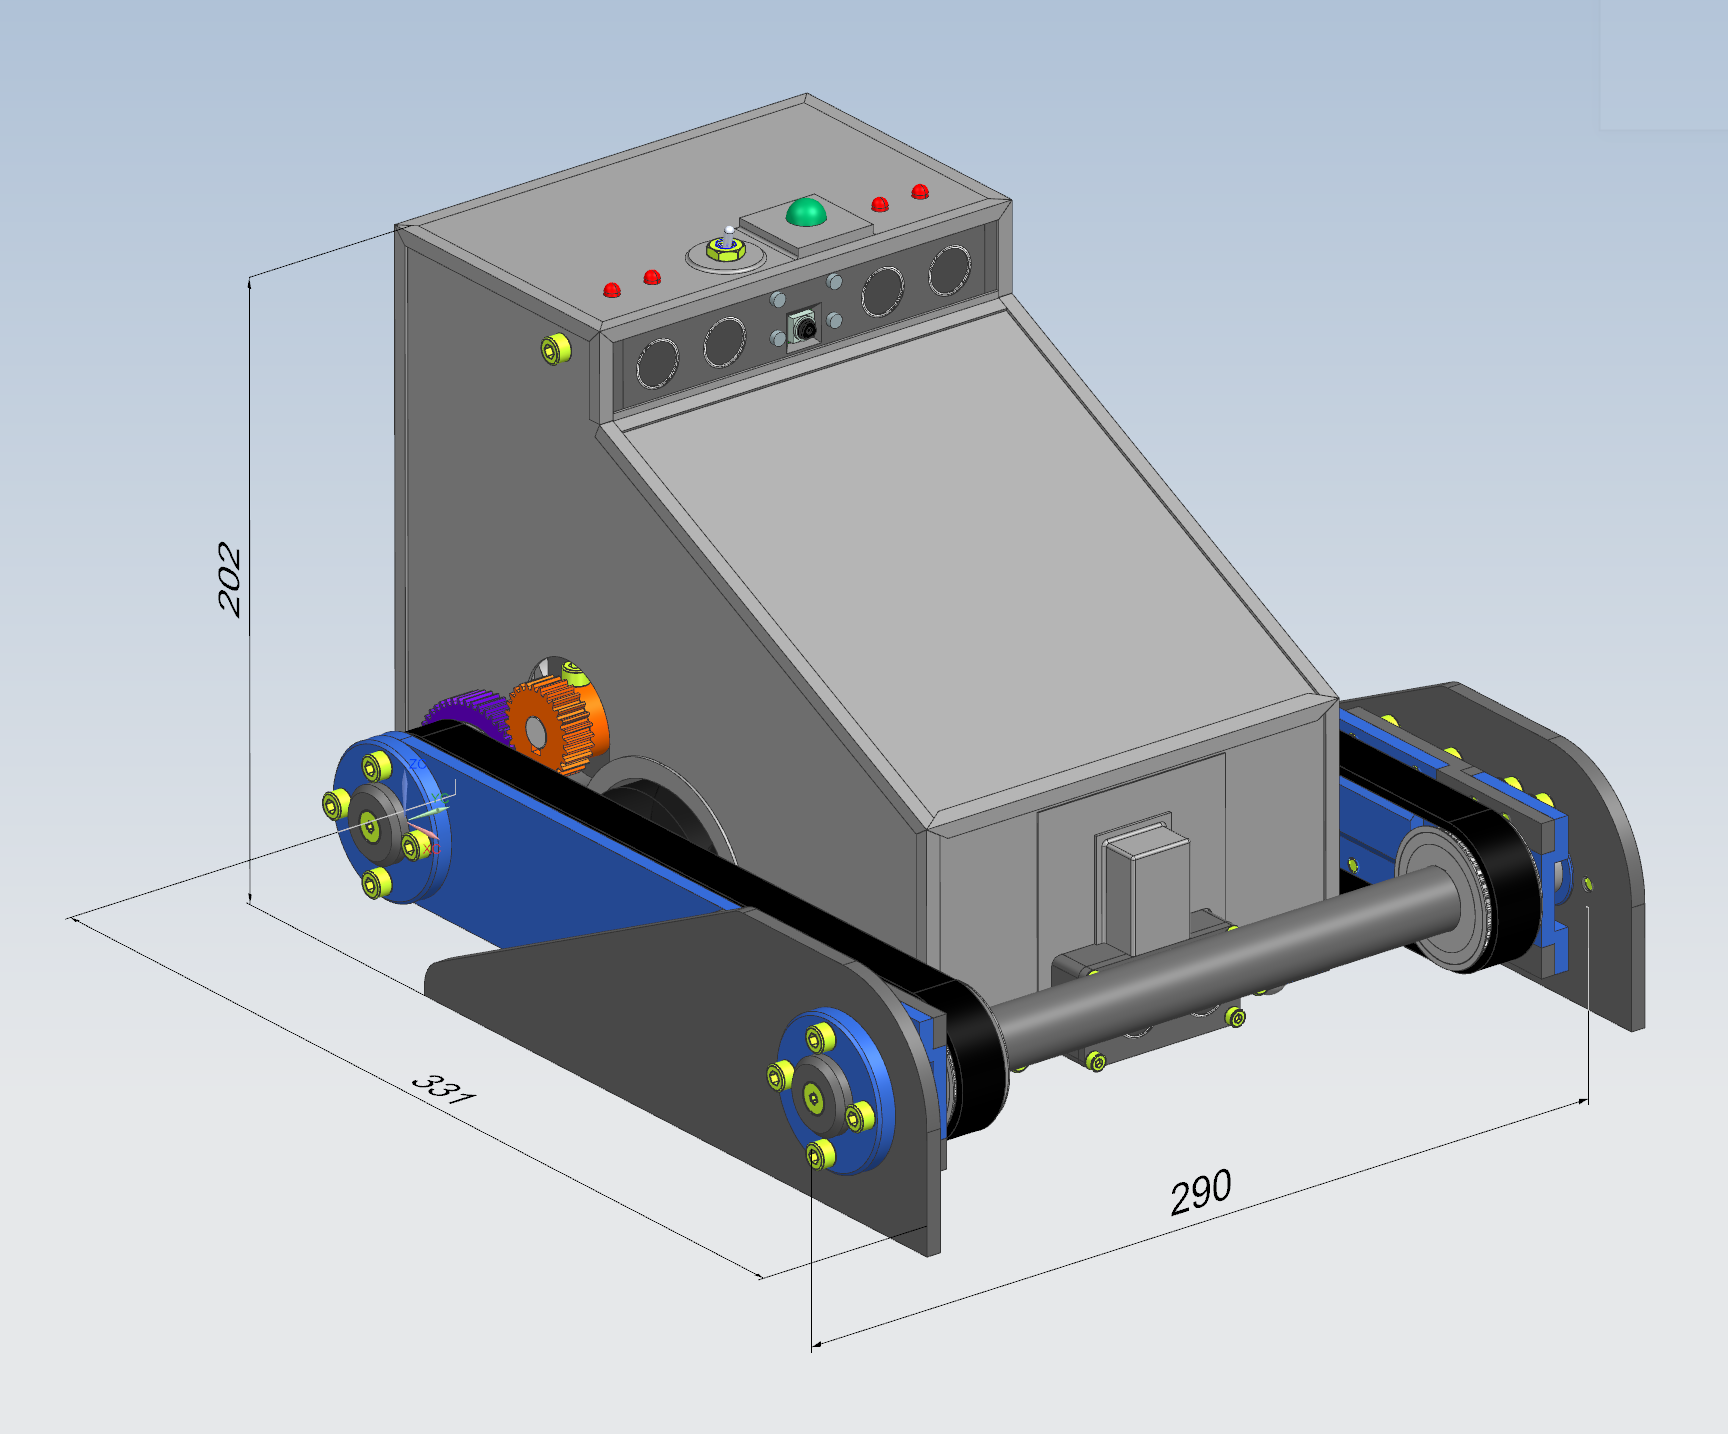
\includegraphics[width=0.9\textwidth]{img/Gerät Aufbau/GerätmitHaubeundMasse.PNG}
  \centering
  \caption{CAD-Modell}
  \label{fig:CADmitMassen}
\end{figure}

Das Gerät hat mit aufgesetzter Haube eine Grösse von 331 mm x 290 mm x 202 mm, wenn sich die Ausleger horizontal zum Grundkörper befinden. Das Gewicht des Geräts beträgt 3.29 kg.

\newpage

In der Abbildung \ref{fig:CADohneHaube1} ist die CAD-Baugruppe seitlich von vorne zusehen und in der Abbildung \ref{fig:CADohneHaube2} seitlich von hinten. Bei beiden Bildern ist das Gerät ohne Haube dargestellt, um den inneren Aufbau ersichtlich zu machen.\\

\begin{figure}[H]
  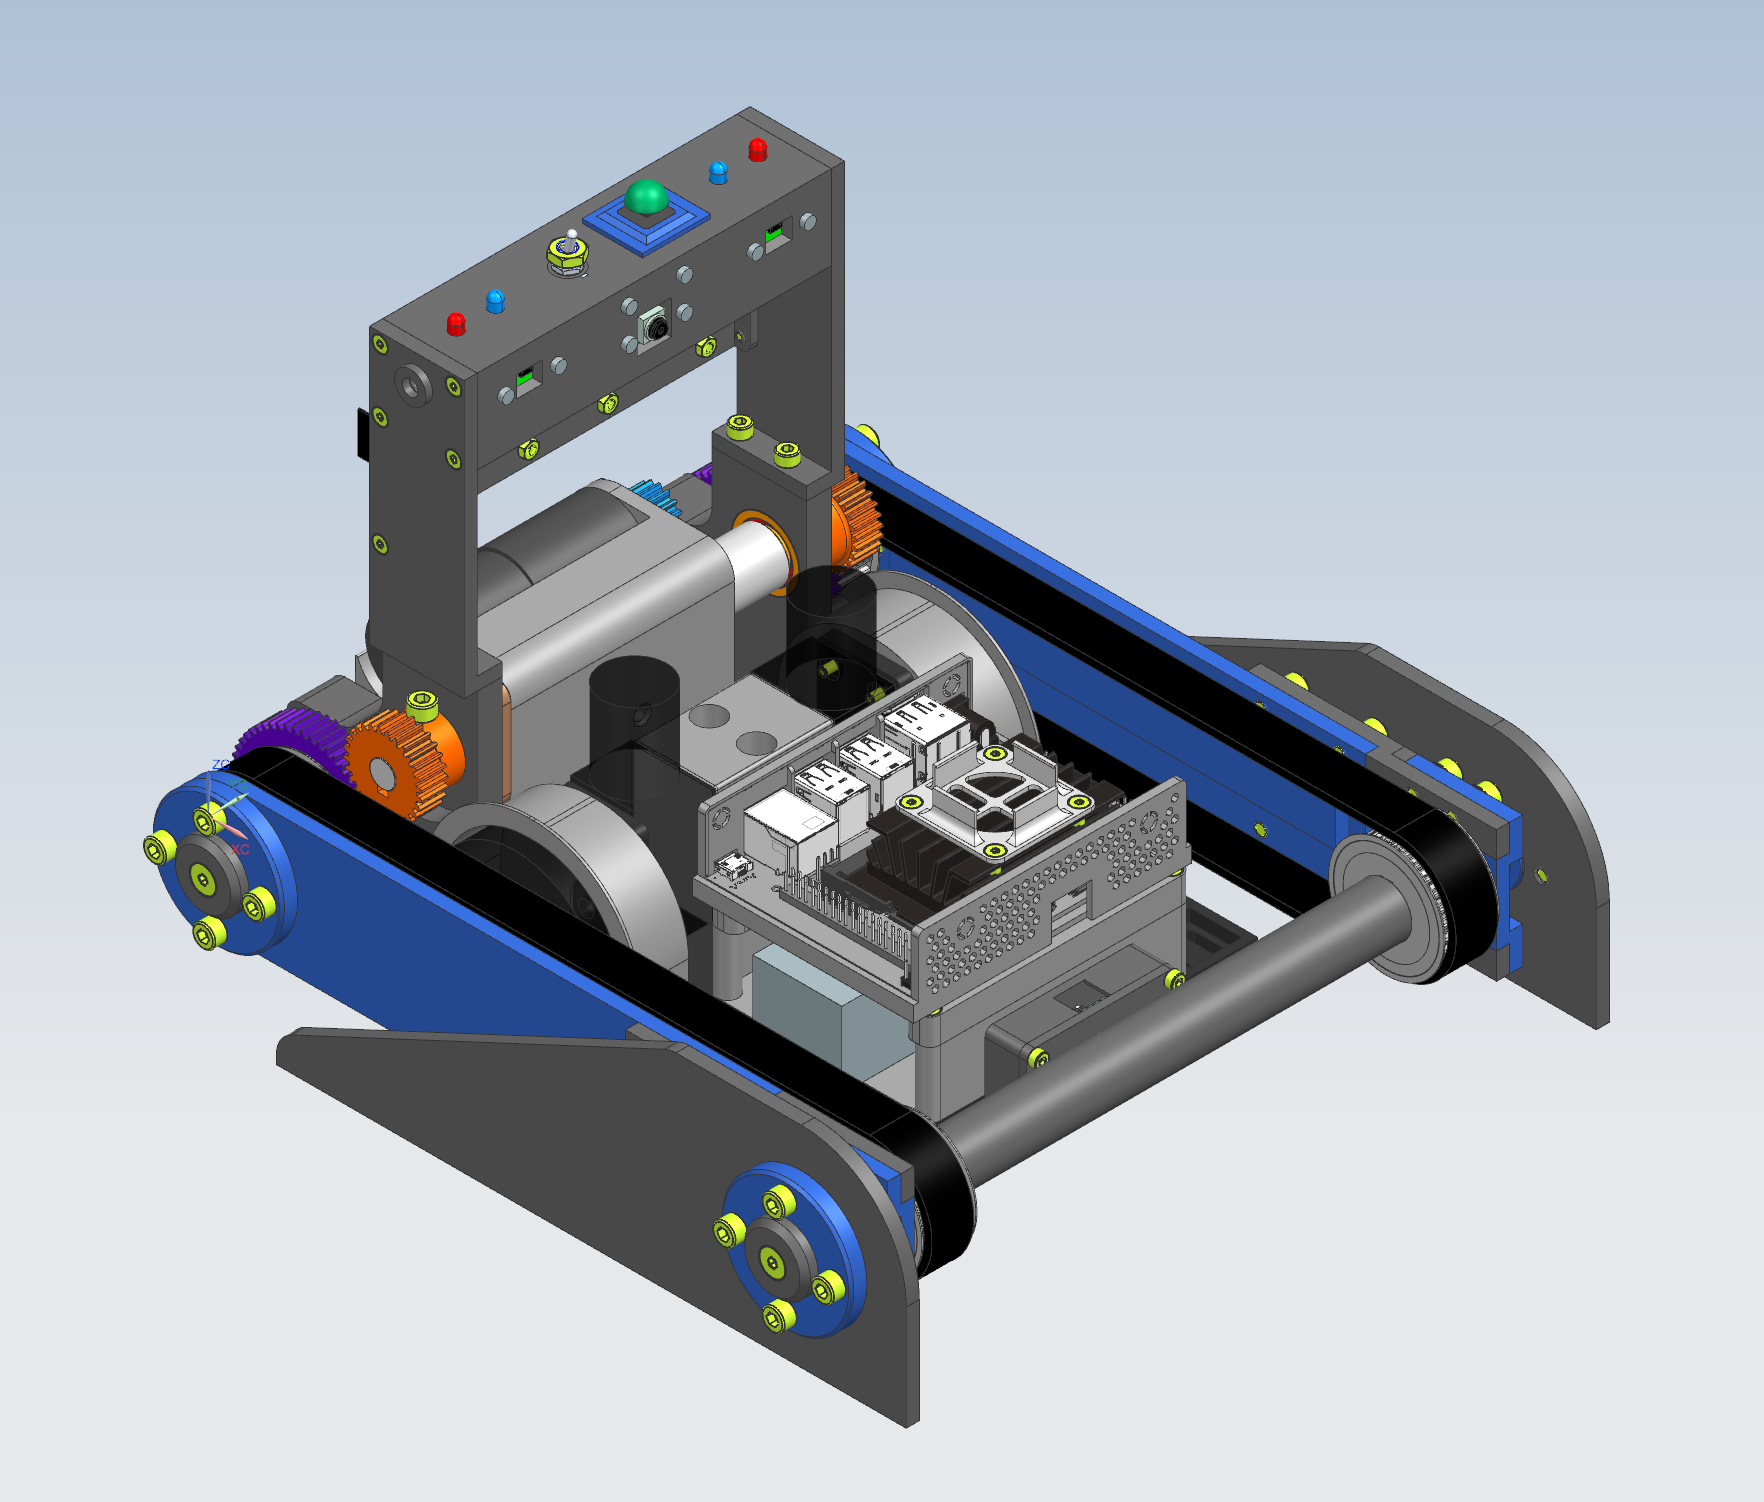
\includegraphics[width=0.9\textwidth]{img/Gerät Aufbau/CADohneHaube1.png}
  \centering
  \caption{CAD-Modell ohne Haube, Ansicht 1}
  \label{fig:CADohneHaube1}
\end{figure}

\begin{figure}[H]
  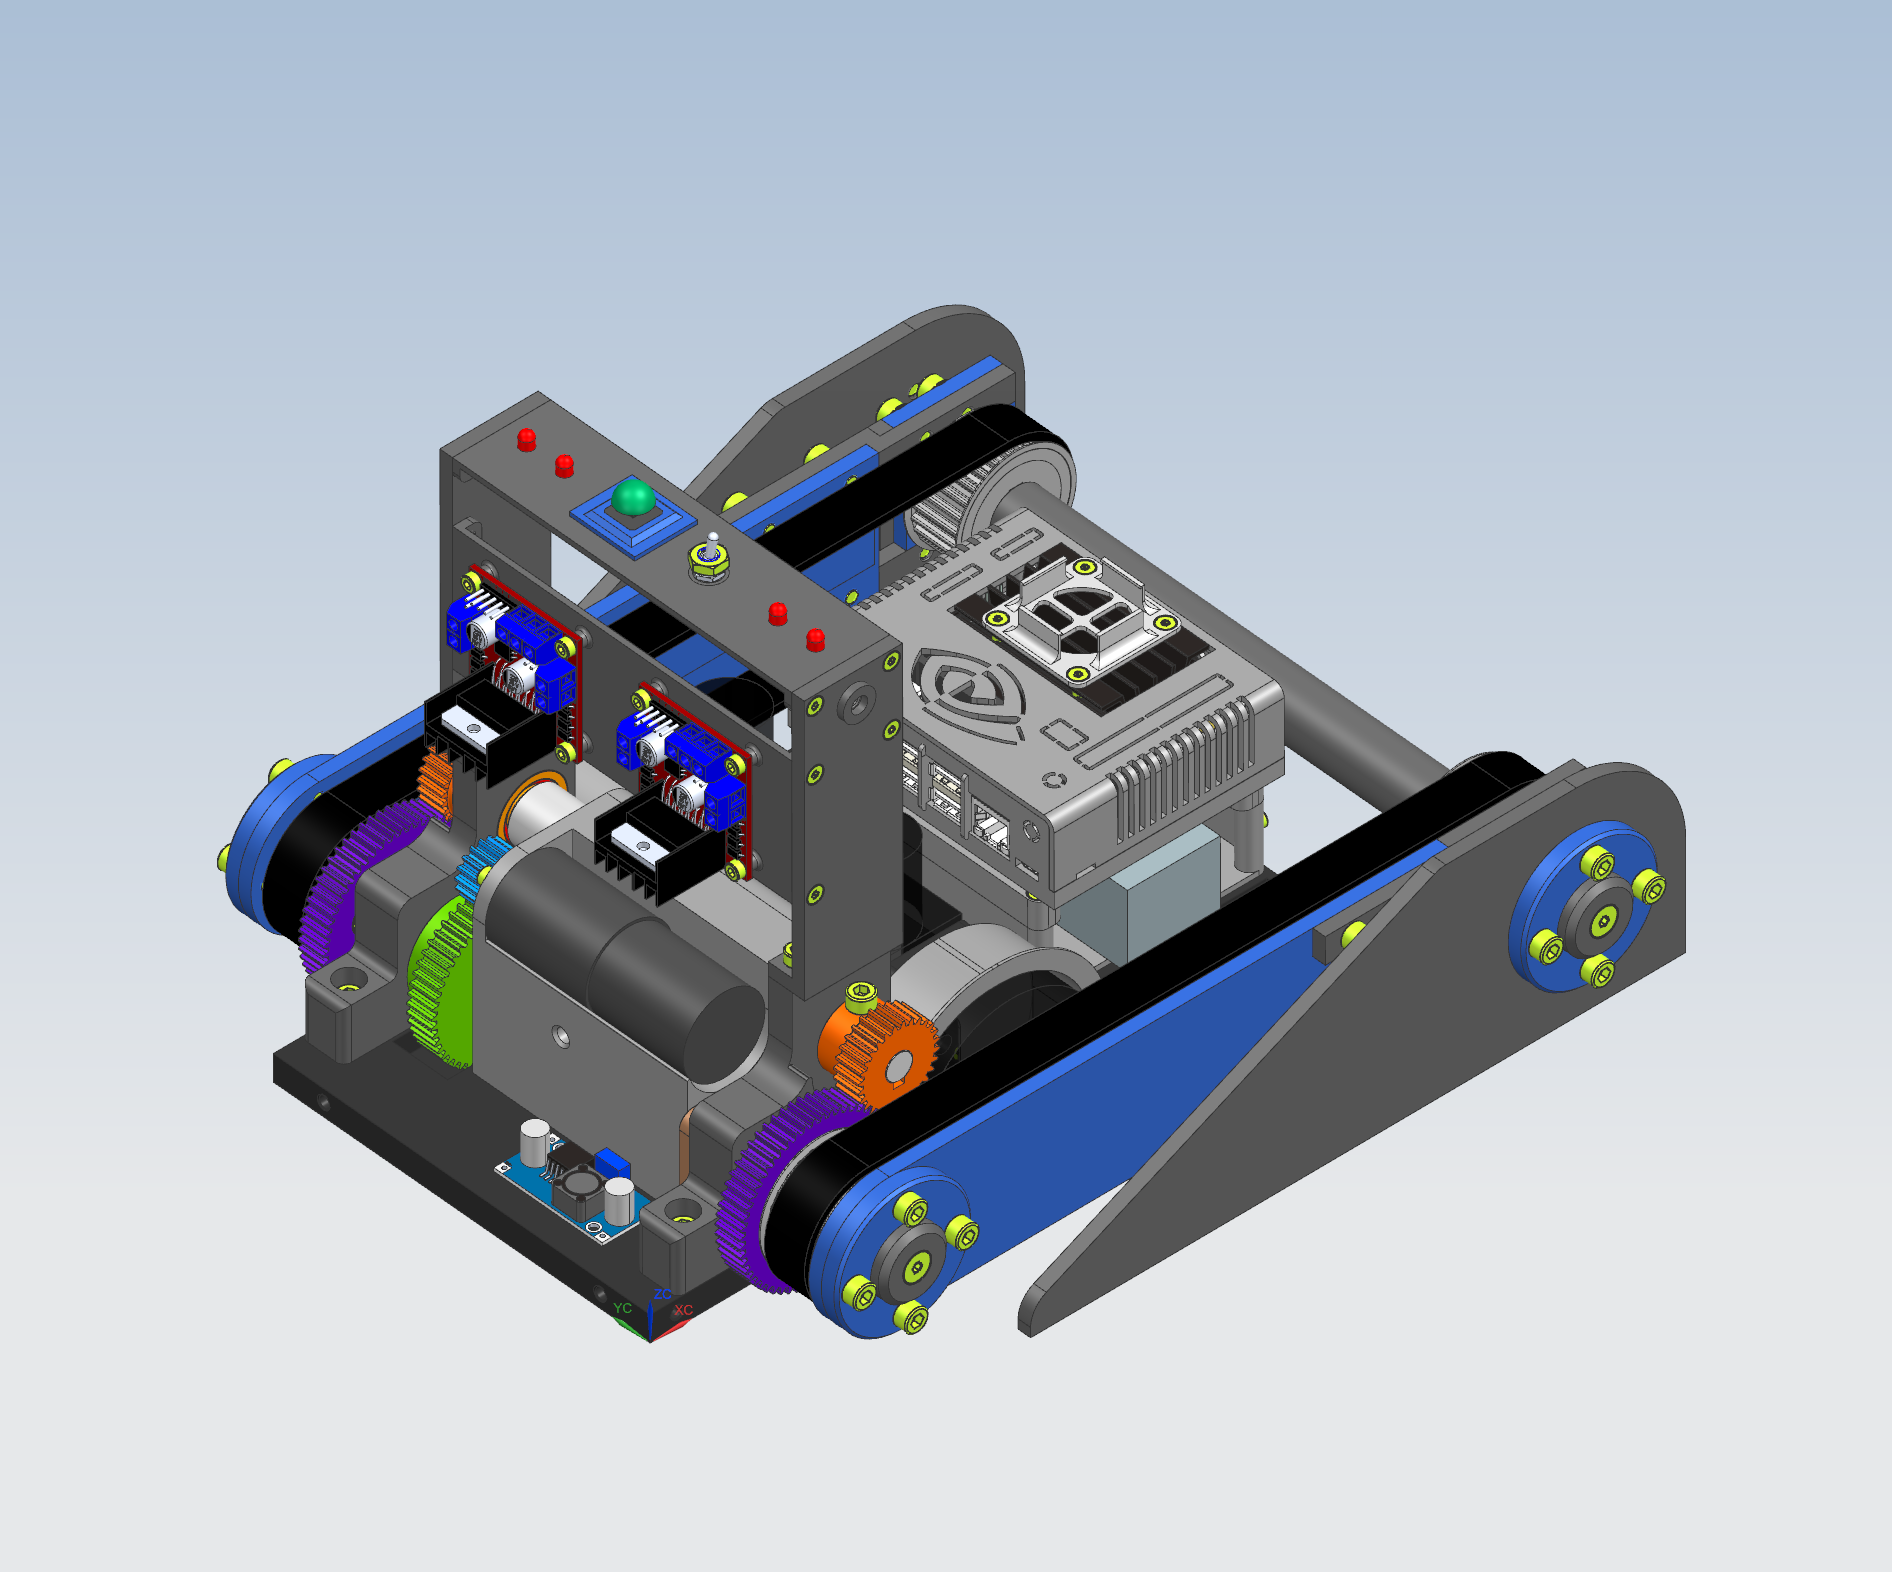
\includegraphics[width=0.9\textwidth]{img/Gerät Aufbau/CADohneHaube2.png}
  \centering
  \caption{CAD-Modell ohne Haube, Ansicht 2}
  \label{fig:CADohneHaube2}
\end{figure}


\subsection{Aufgebautes Gerät}

Die Abbildung \ref{fig:GerätohneHaube} zeigt das aufgebaute Gerät ohne Haube und in der Abbildung \ref{fig:GerätmitHaube} ist das Gerät mit Haube zu sehen. 

\newpage

\begin{figure}[H]
  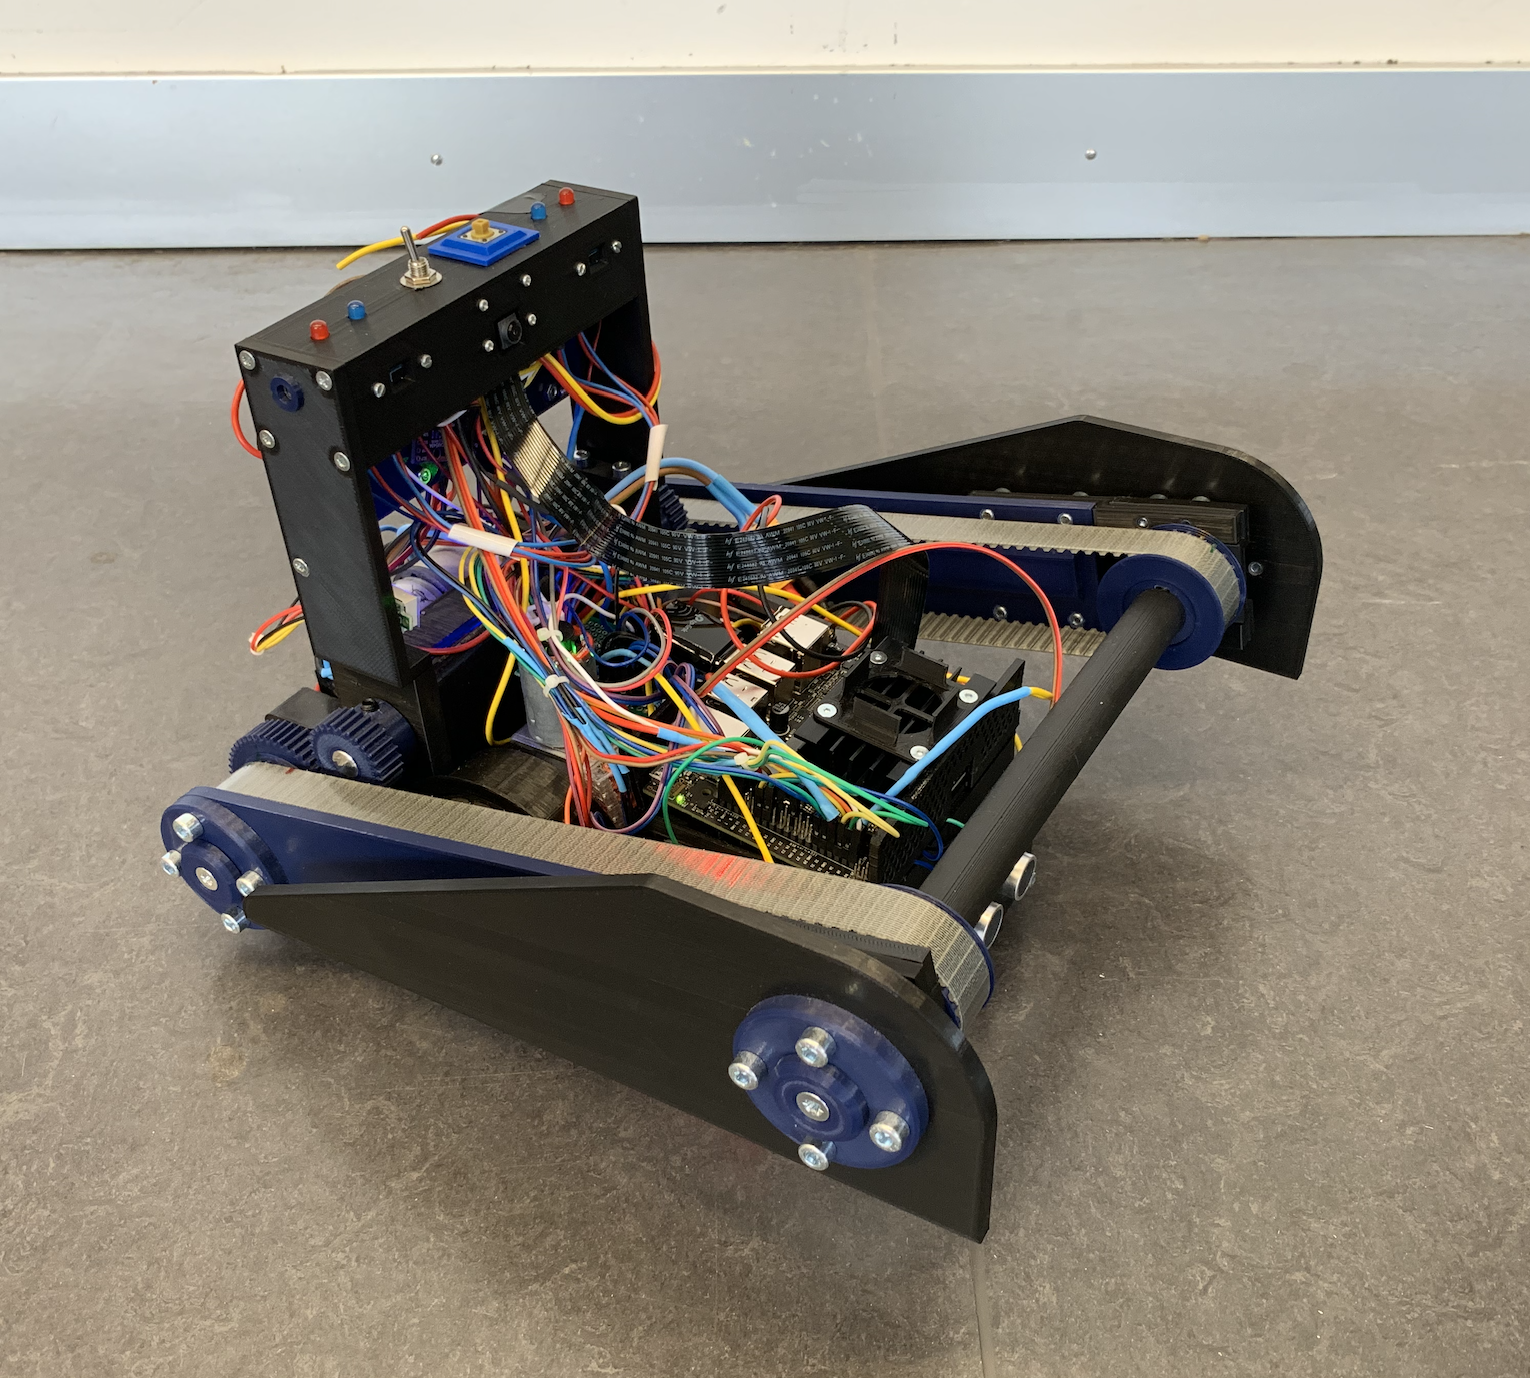
\includegraphics[width=0.9\textwidth]{img/Gerät Aufbau/GerätohneHaube.png}
  \centering
  \caption{Gerät ohne Haube}
  \label{fig:GerätohneHaube}
\end{figure}

\newpage

\begin{figure}[H]
  \includegraphics[width=0.9\textwidth]{img/Gerät Aufbau/GerätmitHaube.png}
  \centering
  \caption{Gerät mit Haube}
  \label{fig:GerätmitHaube}
\end{figure}                        
\newpage

\subsection{Komponenten}
\label{subsec:Komponenten}

In diesen Abschnitt werden die Komponenten des Grundgerüsts gezeigt. Die dazu vorhandenen CAD-Modelle und Zeichnungen sind im abgegebenen ZIP Ordner enthalten.

\textbf{Grundplatte:} Die Grundplatte besteht aus zwei 3D-gedruckten Platten, die zusammengesteckt und verklebt sind. Die notwendigen Bohrungen für Schrauben konnten direkt mitgedruckt werden. Die Halterungen für die Fortbewegungsmotoren sind in die Grundplatte integriert.

\begin{figure}[H]
  \includegraphics[width=0.7\textwidth]{img/Gerät Aufbau/Grundplatte.png}
  \centering
  \caption{Grundplatte}
  \label{fig:Grundplatte}
\end{figure}

\textbf{Wellen:} Die Wellen des Gerätes wurden von der mechanischen Werkstatt der Hochschule gefertigt. Sie sind aus Aluminium. Von den 10 Stunden, welche für die Fertigung in der mechanischen Werkstatt zur Verfügung stehen, wurden 6.5 Stunden für die drei Wellen gebraucht. Die Auslegerwelle wurde jedoch durch eine Kunststoff Welle ersetzt. Dieser Austausch ist im Kapitel \ref{sec:Funktionsweisemit Akku} dokumentiert.

\begin{figure}[H]
  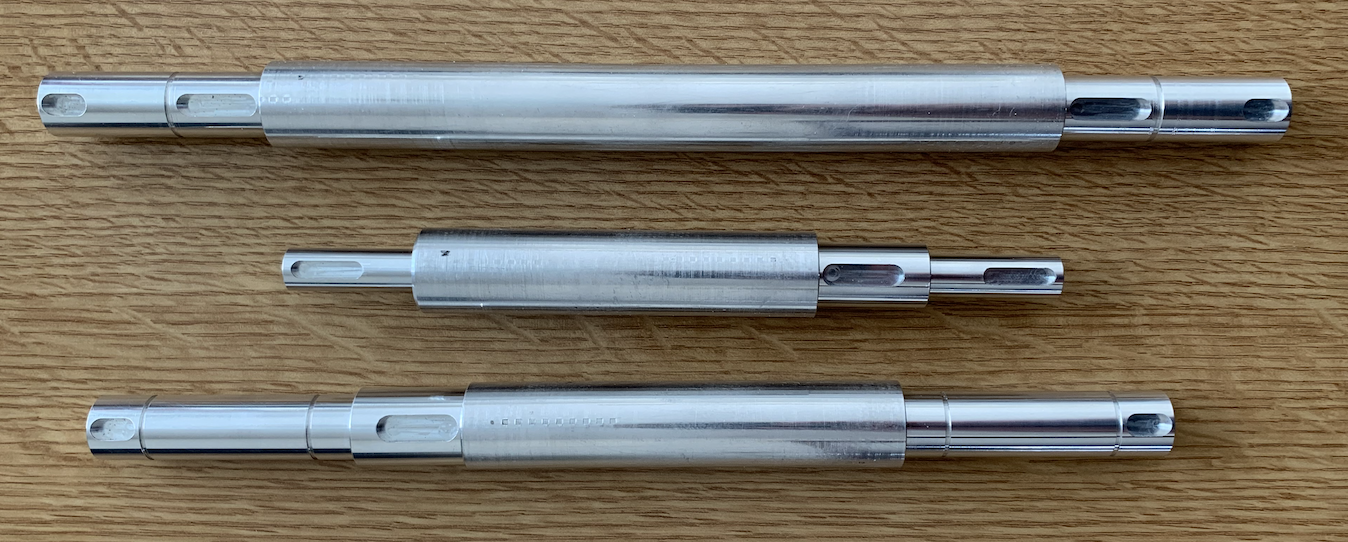
\includegraphics[width=0.7\textwidth]{img/Gerät Aufbau/Wellen.png}
  \centering
  \caption{unten: Welle 1, mitte: Welle 2, oben: Auslegerwelle}
  \label{fig:Wellen}
\end{figure}

\newpage

\textbf{Lagerung der Grundkörperwellen:} An die Grundplatte sind hinten an den Seiten zwei Lagerböcke geschraubt, welche die zwei Wellen (Welle 1 und Welle 2), die durch den Grundkörper verlaufen, aufnehmen. Ein Lagerbock ist so gestaltet, dass die zwei Lager fest sind (Festlager) und der andere so, dass sich die Lager im Lagerbock verschieben können (Loslager). Somit sind die Wellen 1 und 2 statisch bestimmt gelagert. Der Festlagerbock ist in der Abbildung \ref{fig:Festlager} zu sehen. Der Loslagerbock ist identisch aufgebaut, nur können sich die Lager axial verschieben.

\begin{figure}[H]
  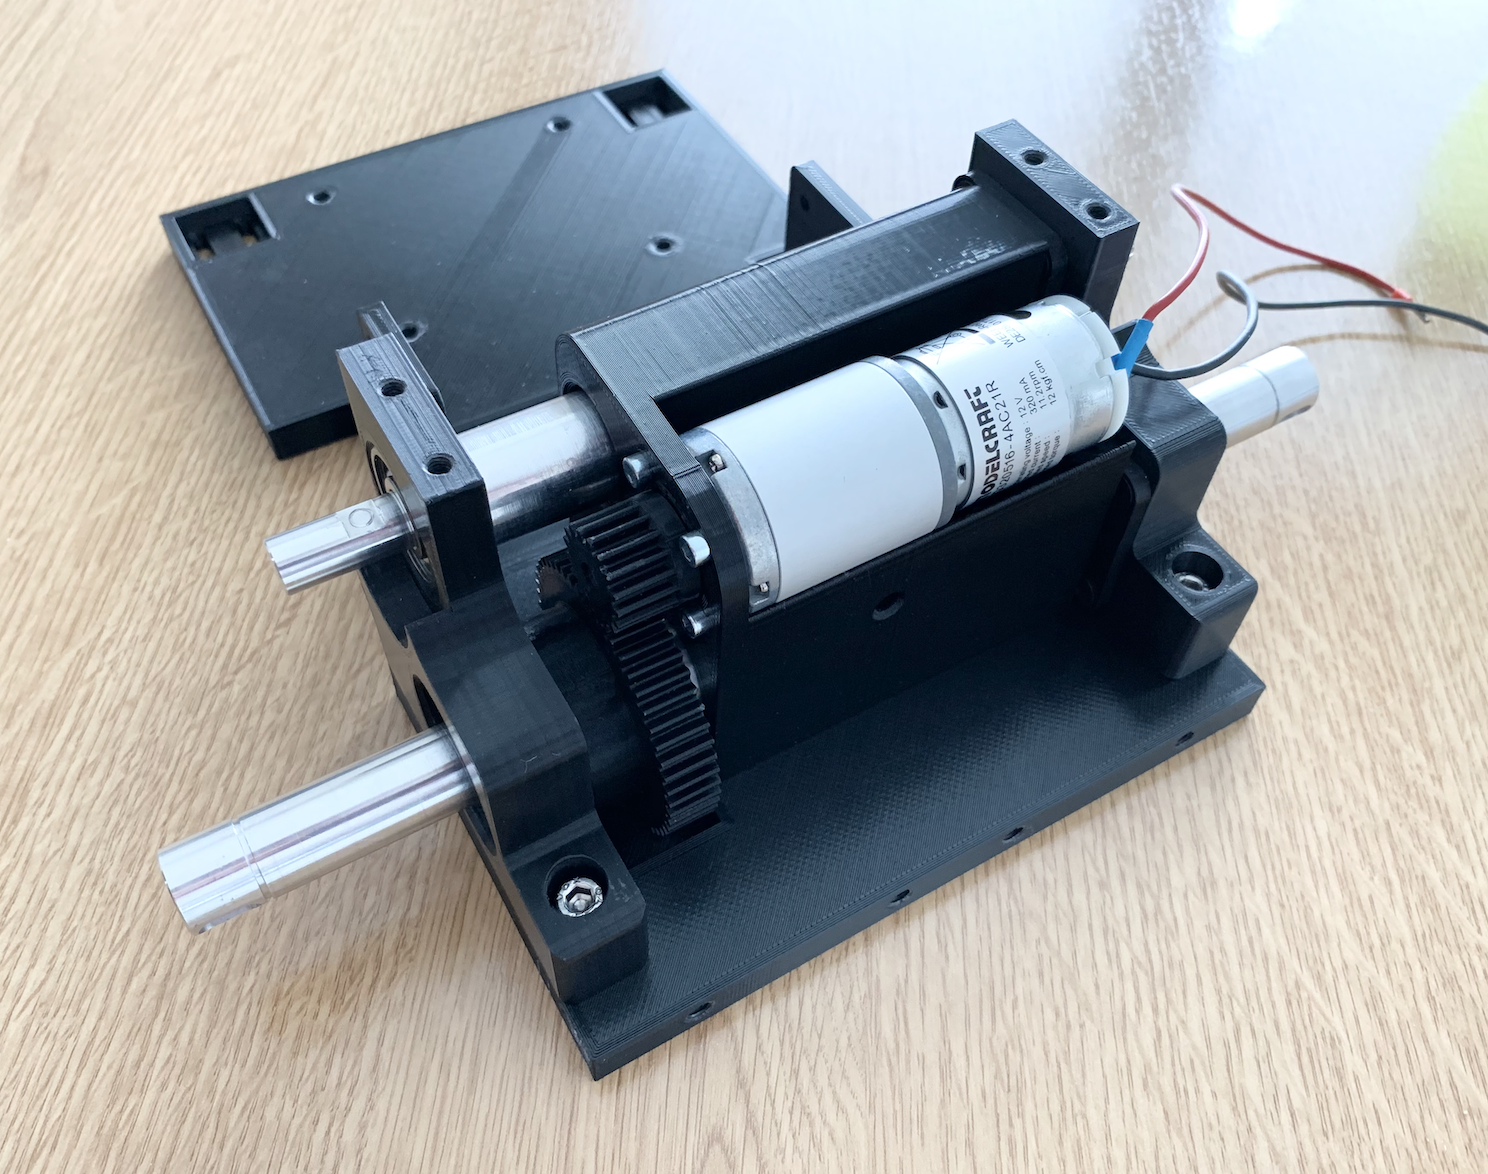
\includegraphics[width=0.7\textwidth]{img/Gerät Aufbau/Lagerböcke.png}
  \centering
  \caption{hinten rechts: Festlager, vorne links: Loslager}
  \label{fig:Lagerung}
\end{figure}

\begin{figure}[H]
  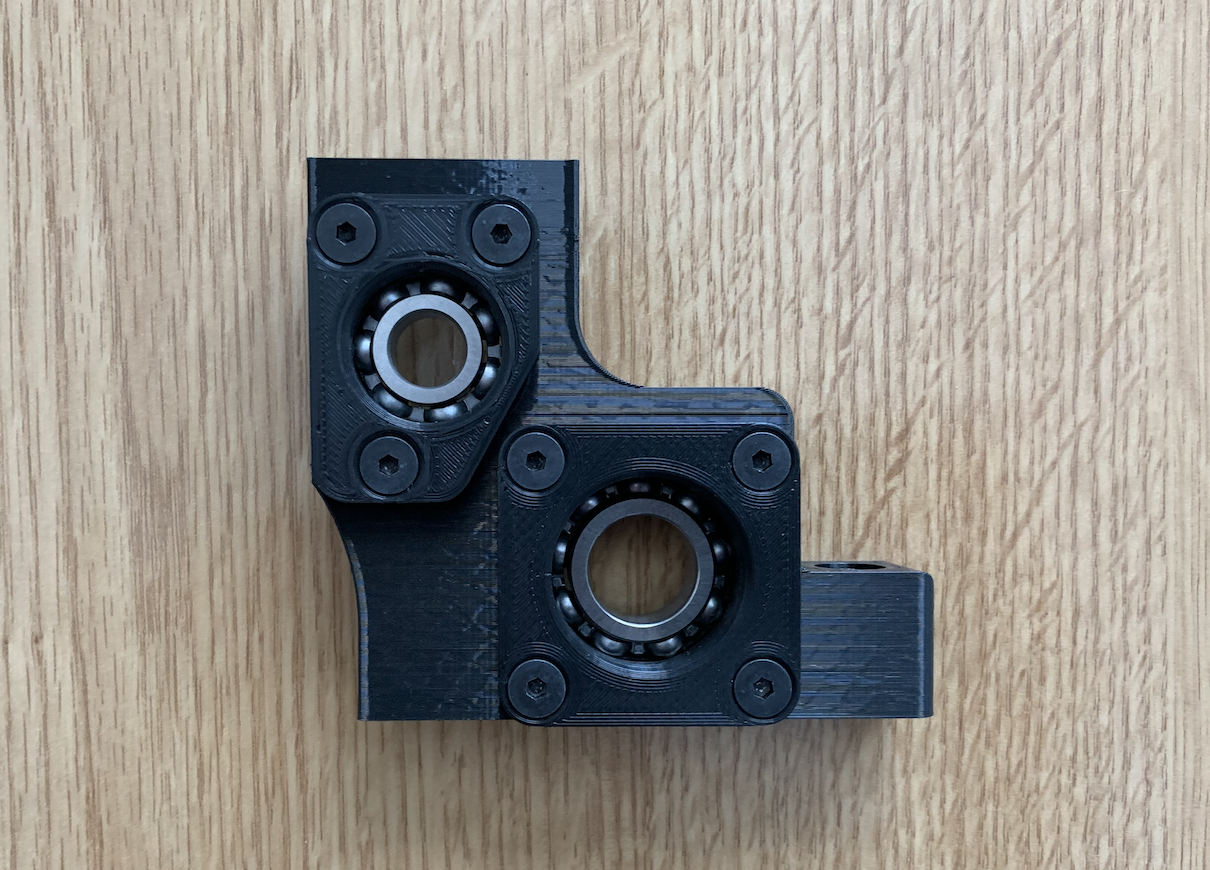
\includegraphics[width=0.5\textwidth]{img/Gerät Aufbau/Festlager.png}
  \centering
  \caption{Lagerbock als Festlager}
  \label{fig:Festlager}
\end{figure}

\newpage

\textbf{Halterung des Hubmotors:} Die Halterung des Hubmotors (siehe Abbildung \ref{fig:Lagerung}) ist 3D-gedruckt. Bei der Halterung ist der Motor mit M3-Schrauben befestigt. Zusätzlich liegt der Motor mantelseitig in der Halterungen auf, um den Motor möglichst stabil halten zu können. Die Halterung ist von unten an die Grundplatte geschraubt.

\textbf{Zahnräder:} Alle Zahnräder, die im Gerät verbaut sind, sind 3D-gedruckt. Tests haben gezeigt, dass die Zahnräder die Belastung aushalten. Dies hat die Vorteile, dass zum einen Gewicht und zum anderen Kosten gespart werden können. Das seitliche Gewinde, das die Zahnräder aufweisen, um mit einer Schraube die axiale Verschiebung zu verhindern, ist mit einer eingesetzten Mutter realisiert (siehe Abbildung \ref{fig:Zahnräder}). Dies ist so gemacht, damit die Innengewinde eine genügend grosse Festigkeit aufweisen. Die Spezifikationen der Zahnräder sind im Anhang unter Kapitel Zahnräder und Zahnriemen zu finden.

\begin{figure}[H]
  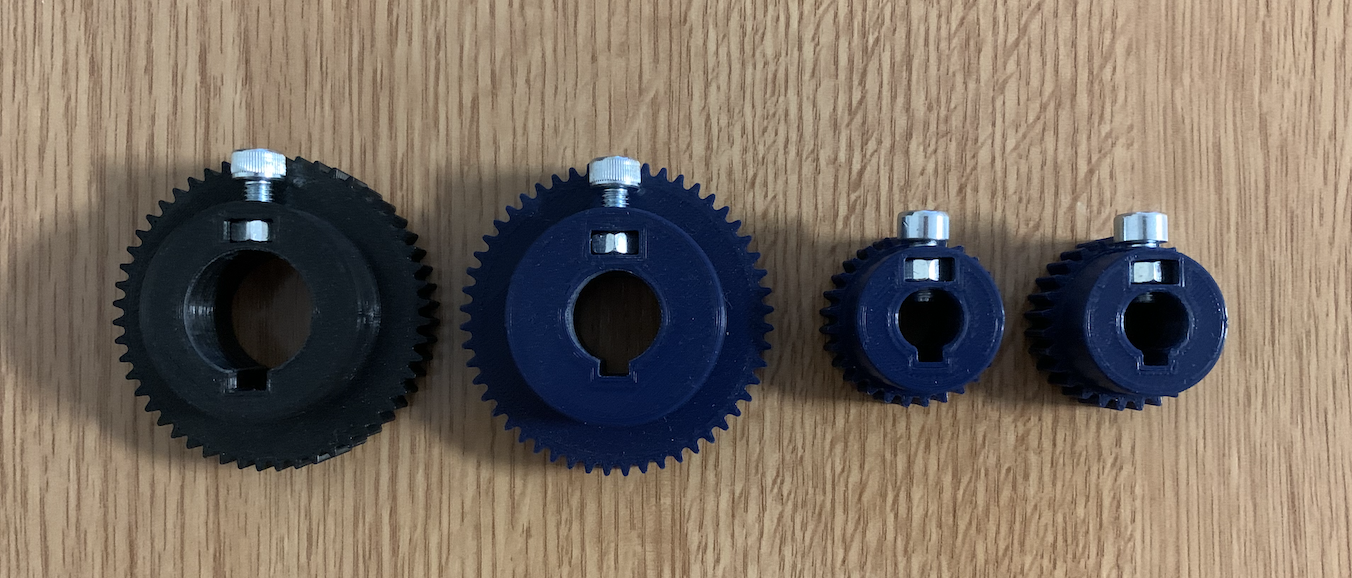
\includegraphics[width=0.9\textwidth]{img/Gerät Aufbau/Zahnräder.png}
  \centering
  \caption{Zahnräder}
  \label{fig:Zahnräder}
\end{figure}

\textbf{Fortbewegung:} Für die Fortbewegung wurden zwei Modellbauräder eingekauft. Die Räder haben einen Durchmesser von 65 mm und sind 32 mm breit. Die Räder sind über ein Verbindungsstück aus Messing mit den Antriebswellen der Fortbewegungsmotoren verbunden. Das Messingstück hat einen Aussensechskant und die Räder einen Innensechskannt. Mit einer Schraube werden die Räder an den Verbindungsstücken gehalten und die Sechskantformverbindung stellt die Mitnahme bei der Drehung sicher. Die Verbindungsstücke sind auf die Motorwellen gesteckt und eine seitliche Schraube, die auf die Freifläche der Motorwelle drückt, ist für die Mitnahme bei der Drehung zuständig. In der Abbildung \ref{fig:Komponenten der Fortbewegung} sind die Komponenten der Fortbewegung zu sehen und in der Abbildung \ref{fig:Räder an Fortbewegungsmotoren} sind die Räder an die Motoren geschraubt.

\begin{figure}[H]
  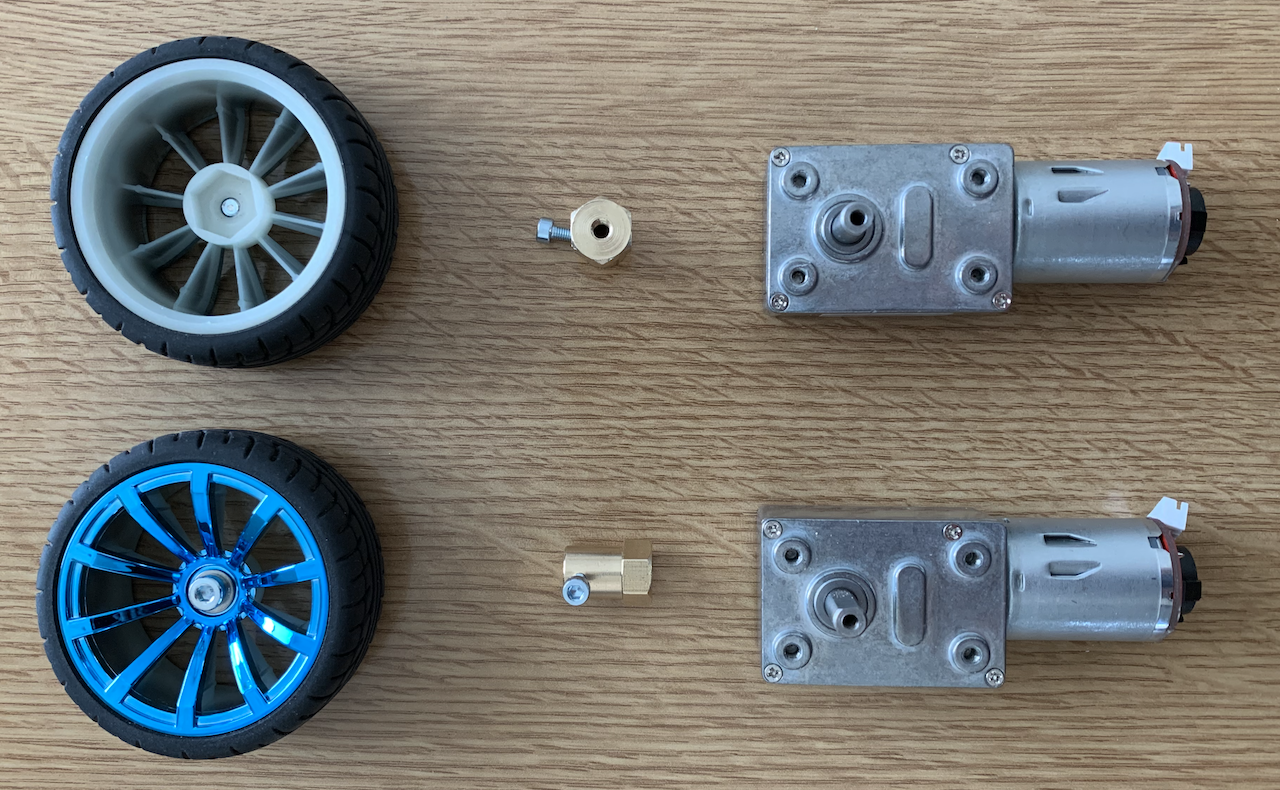
\includegraphics[width=0.8\textwidth]{img/Gerät Aufbau/Räder zerlegt.png}
  \centering
  \caption{Komponenten der Fortbewegung}
  \label{fig:Komponenten der Fortbewegung}
\end{figure}

\begin{figure}[H]
  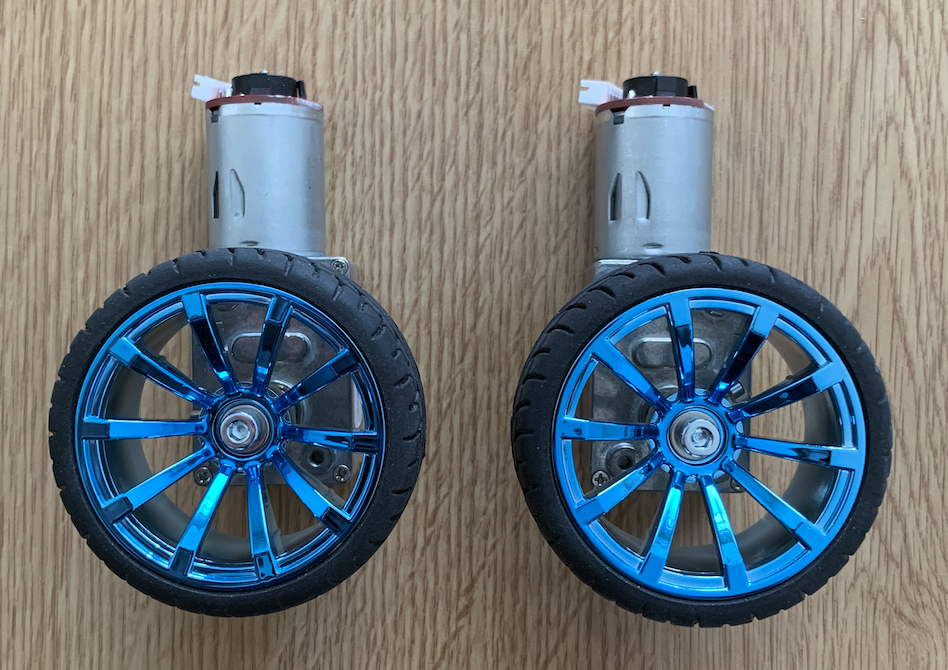
\includegraphics[width=0.8\textwidth]{img/Gerät Aufbau/Räder mit Motor.png}
  \centering
  \caption{Räder an Fortbewegungsmotoren}
  \label{fig:Räder an Fortbewegungsmotoren}
\end{figure}

\newpage

\textbf{Ausleger:} Die seitlichen zwei Ausleger bestehen jeweils aus einer Verbindungsleiste und einem Standfuss. Sie sind über die Auslegerwelle miteinander verbunden.

\begin{figure}[H]
  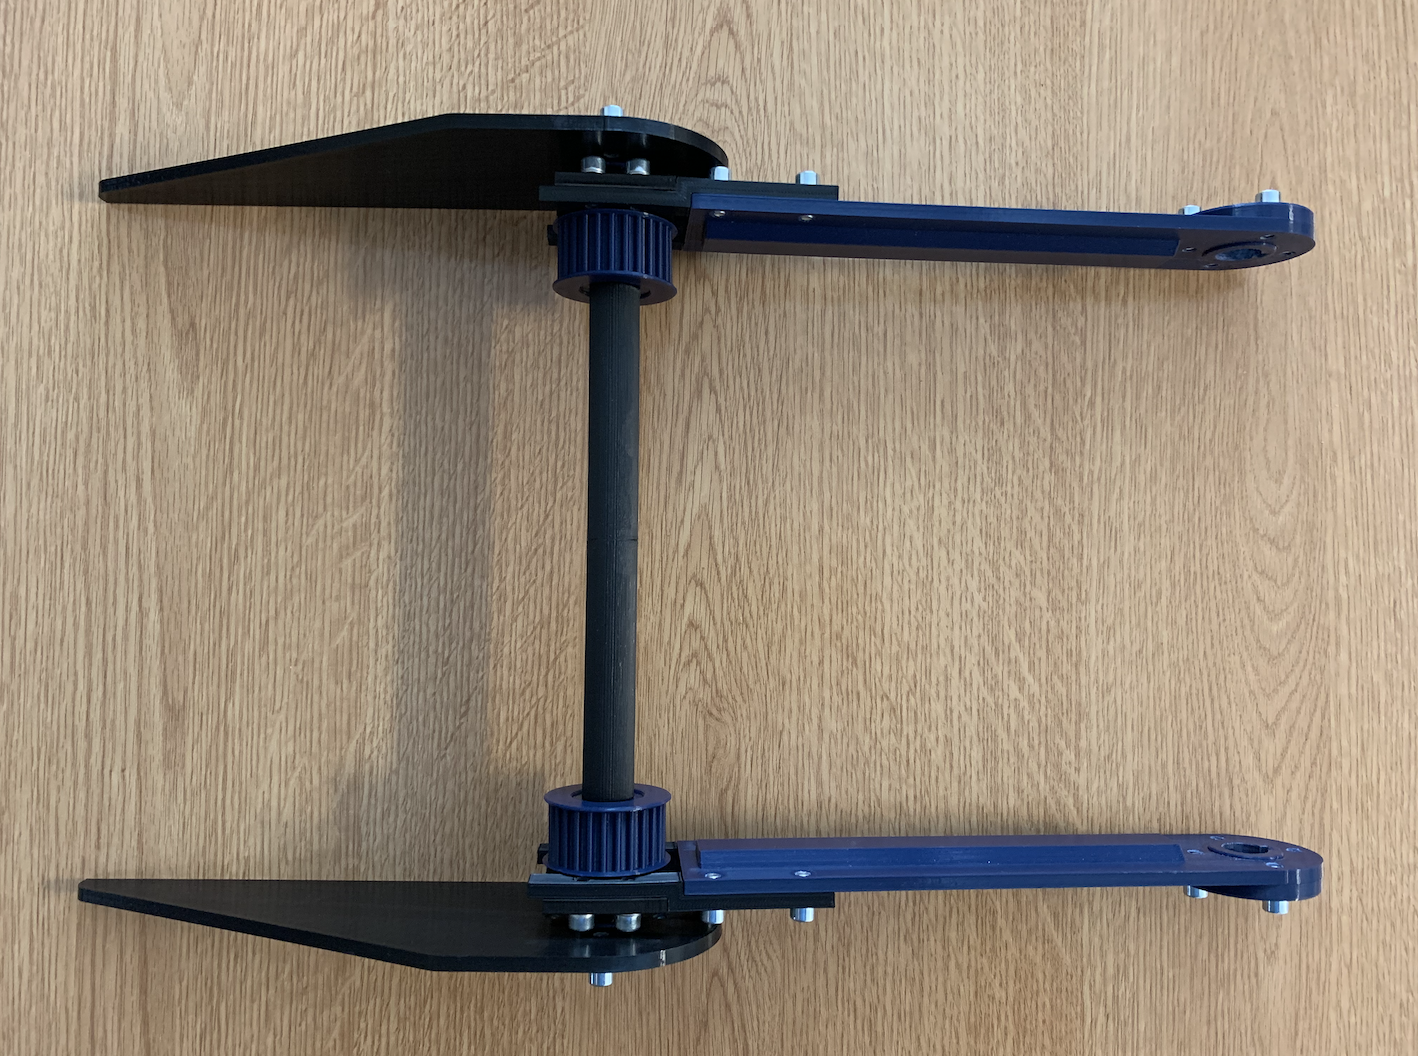
\includegraphics[width=0.8\textwidth]{img/Gerät Aufbau/Ausleger.png}
  \centering
  \caption{Ausleger}
  \label{fig:Ausleger}
\end{figure}

\textbf{Verbindungsleisten:} Die Verbindungsleisten bestehen aus einer Leiste, einem angeschraubten Flansch und angeschraubten Führungen. Die Komponenten der Verbindungsleisten sind 3D-gedruckt.

\begin{figure}[H]
  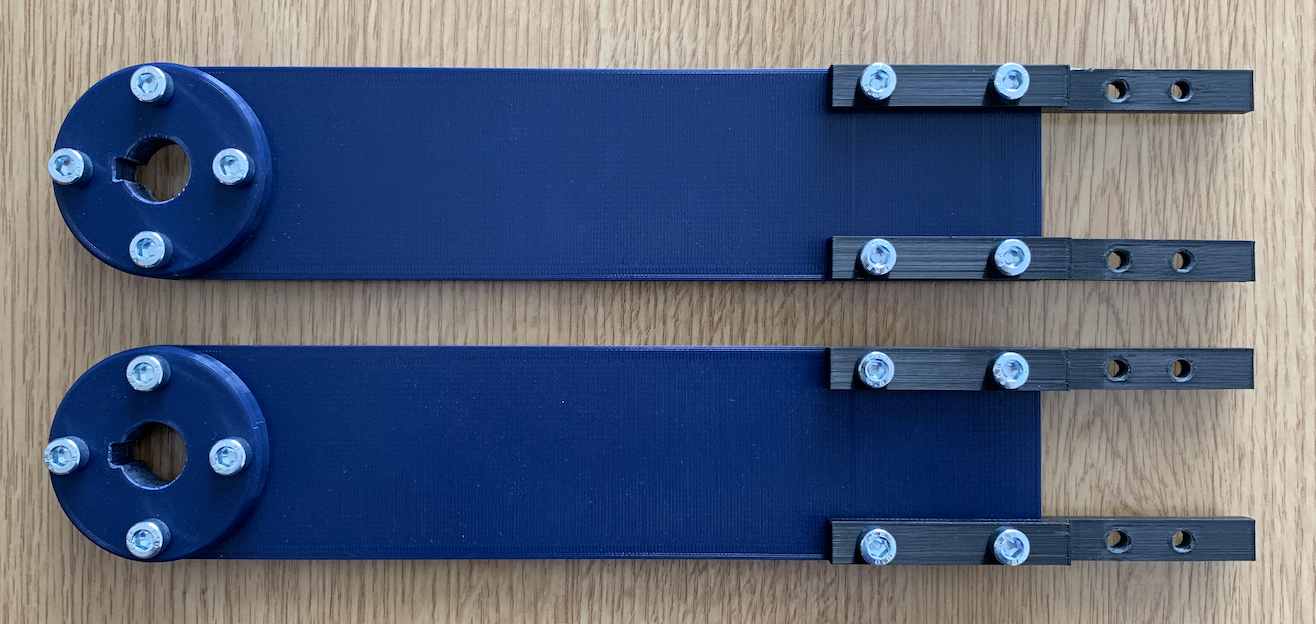
\includegraphics[width=0.8\textwidth]{img/Gerät Aufbau/Verbindungsleisten.png}
  \centering
  \caption{Verbindungsleisten mit angeschraubten Flanschen}
  \label{fig:Verbindungsleisten}
\end{figure}

\textbf{Standfüsse:} Die Standfüsse bestehen aus einem Blech und einem angeschraubten Flansch. Der Flansch ist identisch wie dieser, der bei den Verbindungsleisten eingesetzt ist. Die Standfüsse sind 3D-gedruckt.

\begin{figure}[H]
  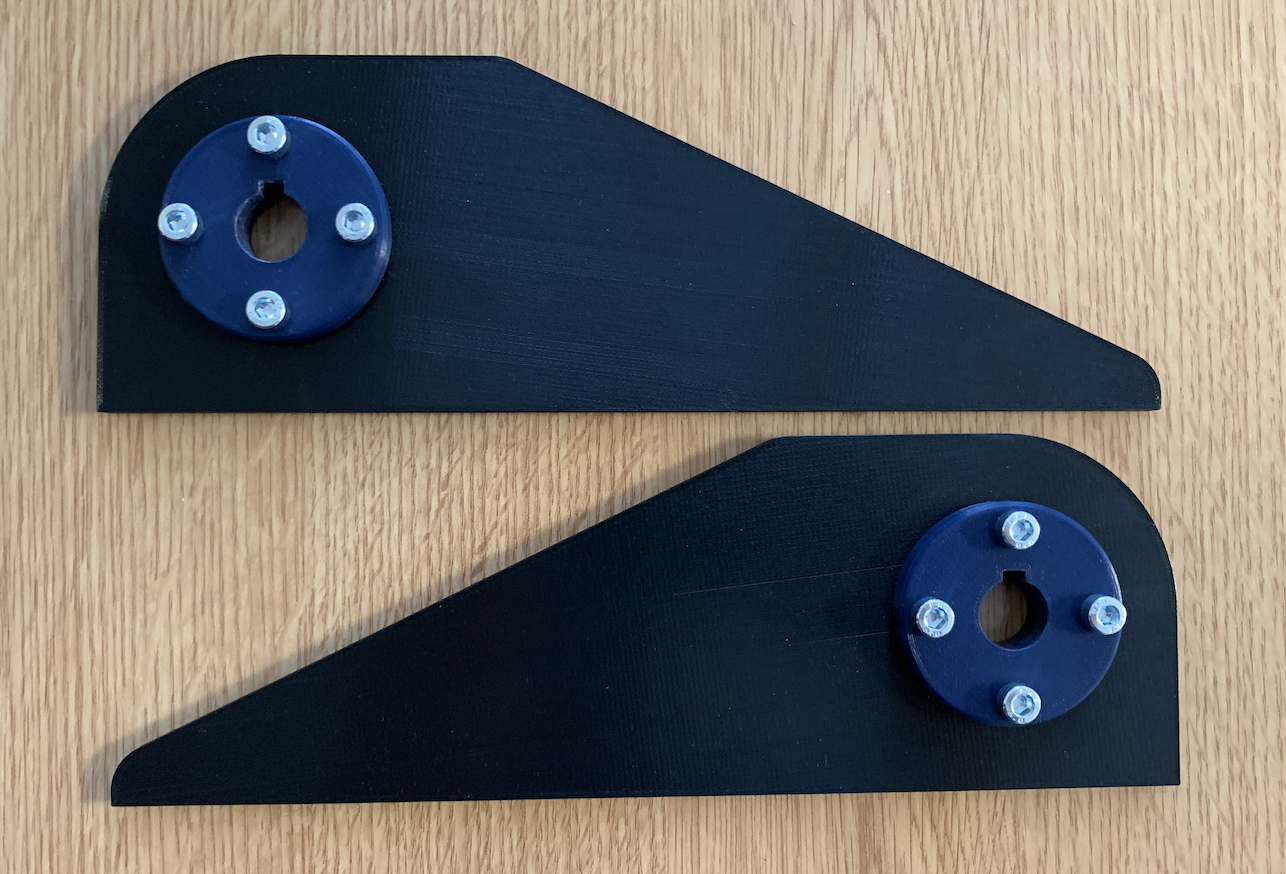
\includegraphics[width=0.8\textwidth]{img/Gerät Aufbau/Standfüsse.png}
  \centering
  \caption{Standfüsse}
  \label{fig:Standfüsse}
\end{figure}

\newpage

\textbf{Auslegerwelle:} Auf der Auslegerwelle (siehe Abbildung \ref{fig:Auslegerwelle}), die 3D-gedruckt ist, sind auf beiden Seiten die Abtriebsräder der Zahnriemen aufgesteckt. Sie besitzen eine Passfederverbindung. Weiter sind die Aufnahmestücke der Verbindungsleisten, die drehbar auf der Welle sitzen, aufgesteckt. Diese Aufnahmestücke enthalten in der Mitte ein Lager, was in der Abbildung \ref{fig:Aufnahmestück} zu sehen ist. Aussen werden erst auf beiden Seiten eine Distanzbüchse und anschliessend die Standfüsse aufgesteckt. Die Standfüsse sind über eine Passfeder mit der Auslegerwelle verbunden.

\begin{figure}[H]
  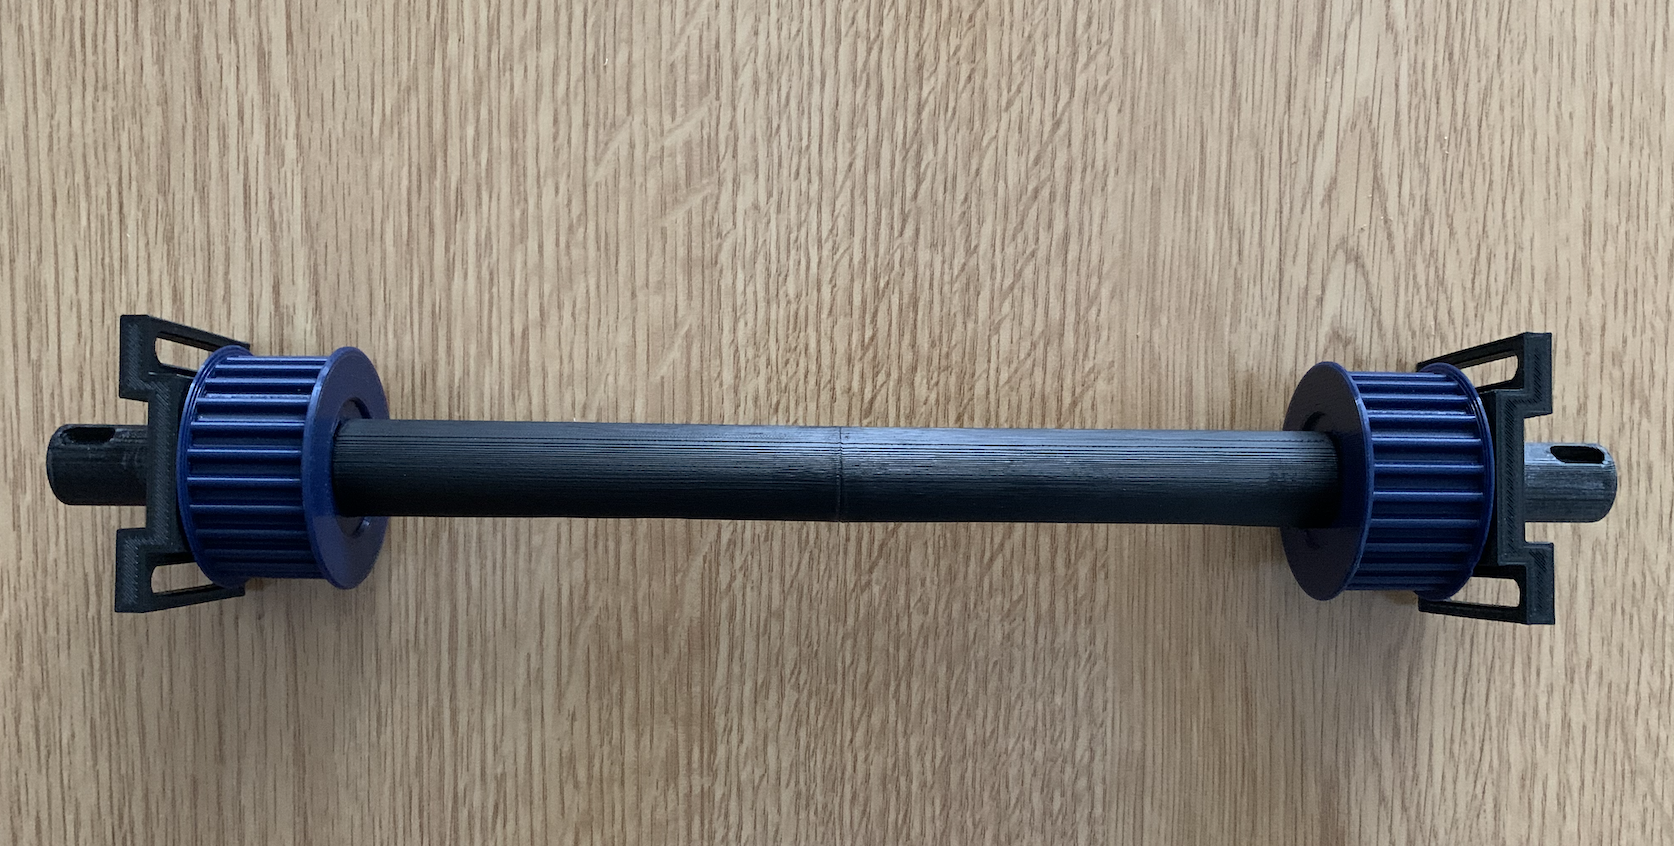
\includegraphics[width=0.8\textwidth]{img/Gerät Aufbau/Auslegerwelle.png}
  \centering
  \caption{Auslegerwelle}
  \label{fig:Auslegerwelle}
\end{figure}

\begin{figure}[H]
  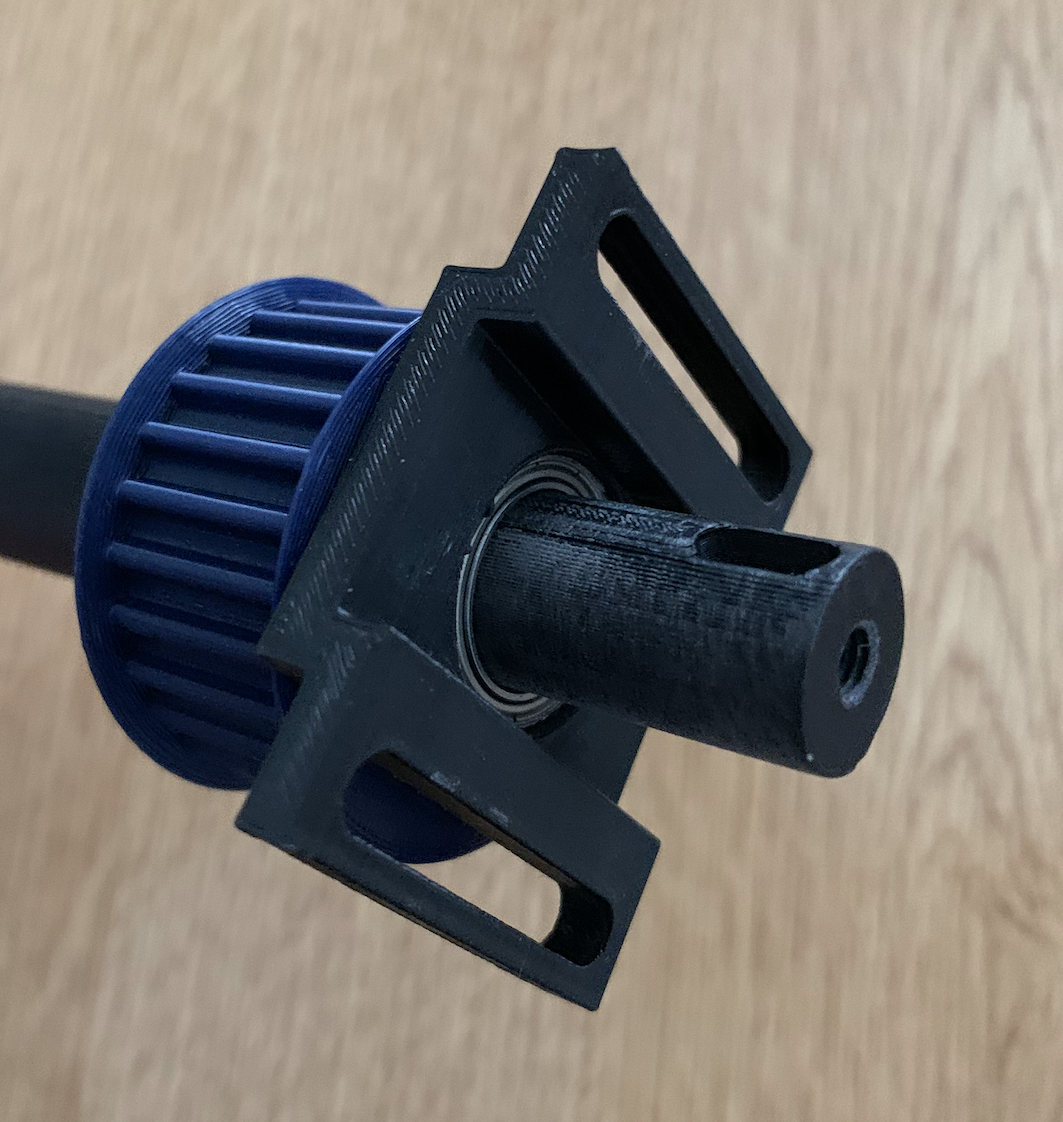
\includegraphics[width=0.5\textwidth]{img/Gerät Aufbau/Aufnahmestück.png}
  \centering
  \caption{Auslegerwelle-Aufnahmestück}
  \label{fig:Aufnahmestück}
\end{figure}

\newpage

\textbf{Zahnriementrieb:} Die Zahnriemen sind auf beiden Seiten des Geräts zwischen der Welle 1 und der Auslegerwelle gespannt. Das treibende Zahnriemenrad sitzt drehbar auf der Welle 1 und das getriebene Zahnriemenrad ist auf der Auslegerwelle fixiert. Die Spezifikationen zu den Zahnriemen sind im Anhang unter Kapitel Zahnräder und Zahnriemen zu finden.

\begin{figure}[H]
  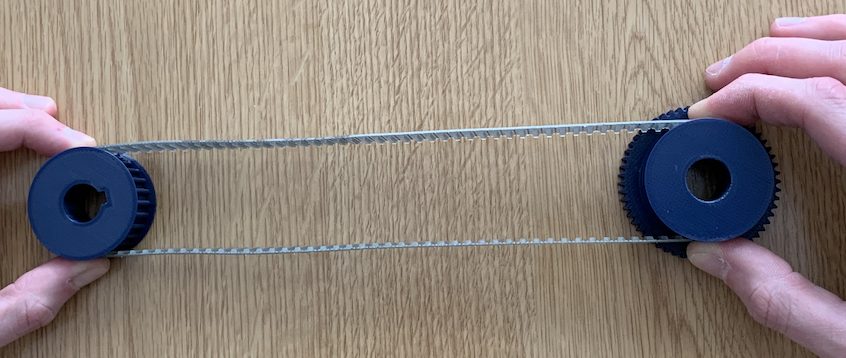
\includegraphics[width=0.8\textwidth]{img/Gerät Aufbau/Zahnriementrieb.png}
  \centering
  \caption{Zahnriementrieb}
  \label{fig:Zahnriementrieb}
\end{figure}

Die Zahnriemen, sind mithilfe eines Einlegestücks gespannt. Diese Methode zum Spannen der Zahnriemen wurde experimentell getestet. Es stellte sich heraus, dass die Spannung, die so erreicht werden kann, ausreicht.

\begin{figure}[H]
  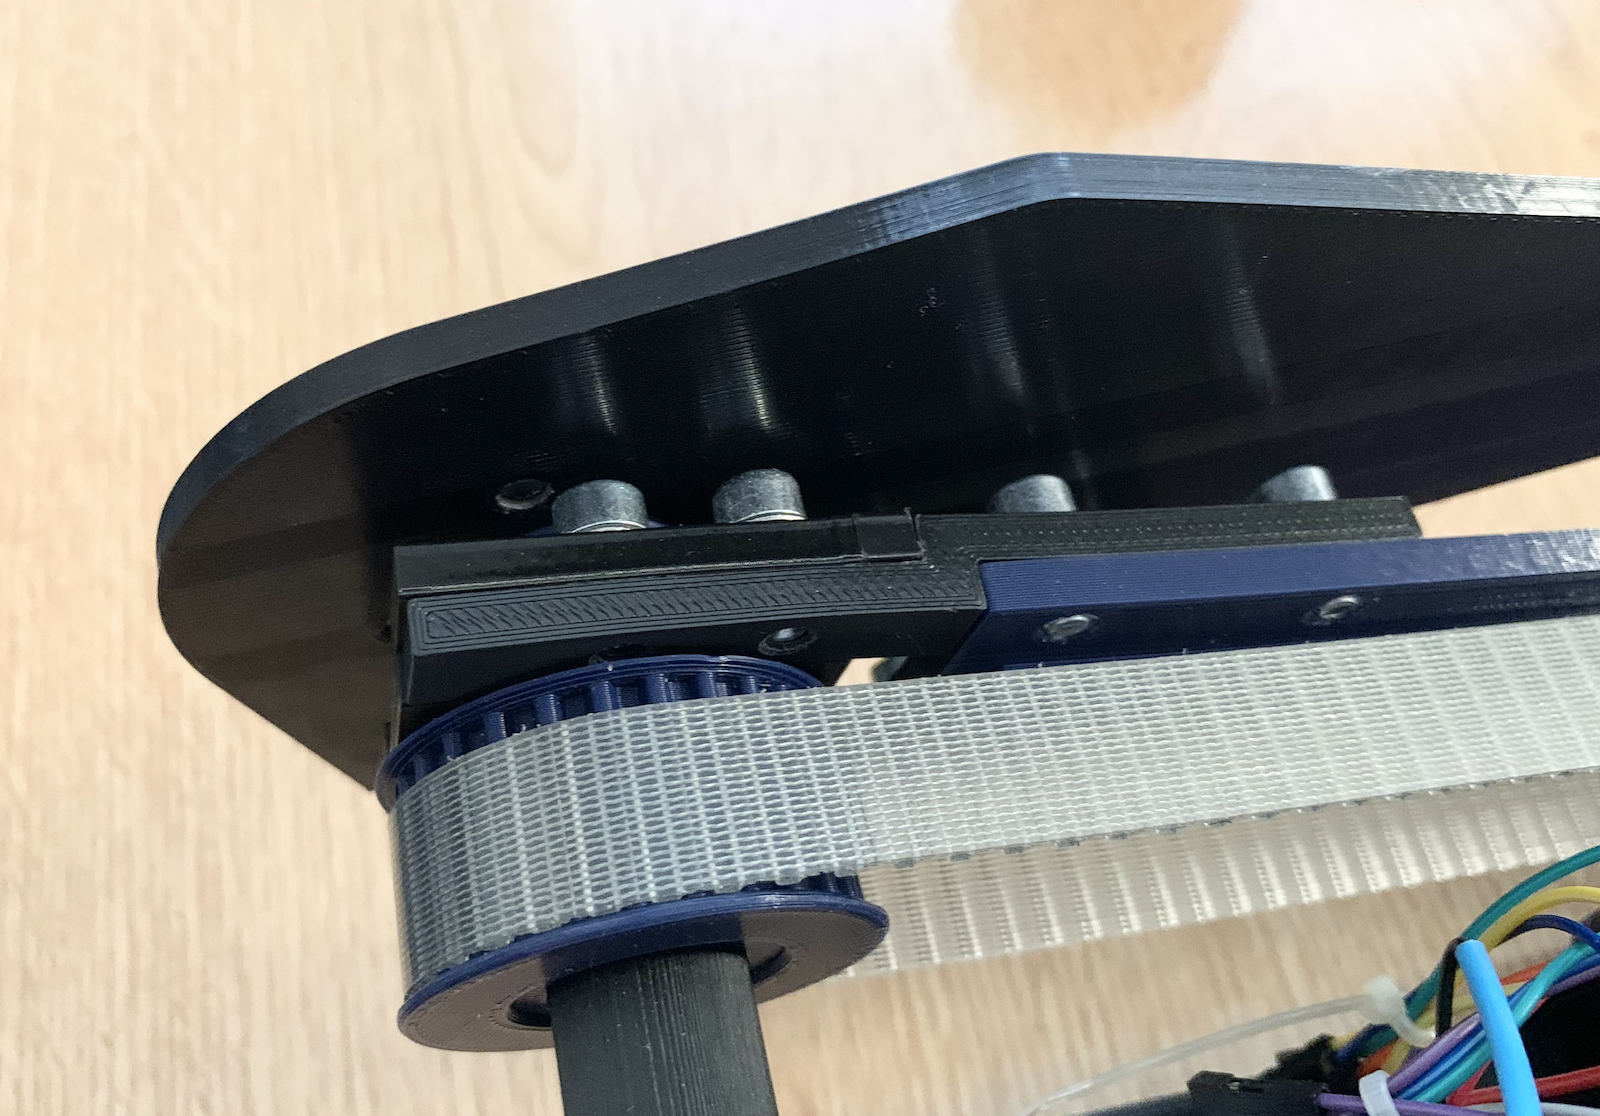
\includegraphics[width=0.8\textwidth]{img/Gerät Aufbau/Zahnriemenspanner.png}
  \centering
  \caption{Methode zum Spannen der Zahnriemen}
  \label{fig:Methode zum Spannen}
\end{figure}

\newpage




\textbf{Akkugehäuse und Bordhalterung:} Der Akku, der die Energiequelle des Geräts ist, ist in einem Gehäuse direkt auf der Grundplatte montiert. Das Gehäuse für das Jetson-Bord ist auf dem Akkugehäuse befestigt. Für die Kühlung des Boards wird ein Ventilator verwendet, für dessen Montage ein Adapter konstruiert und gedruckt wurde.

\begin{figure}[H]
  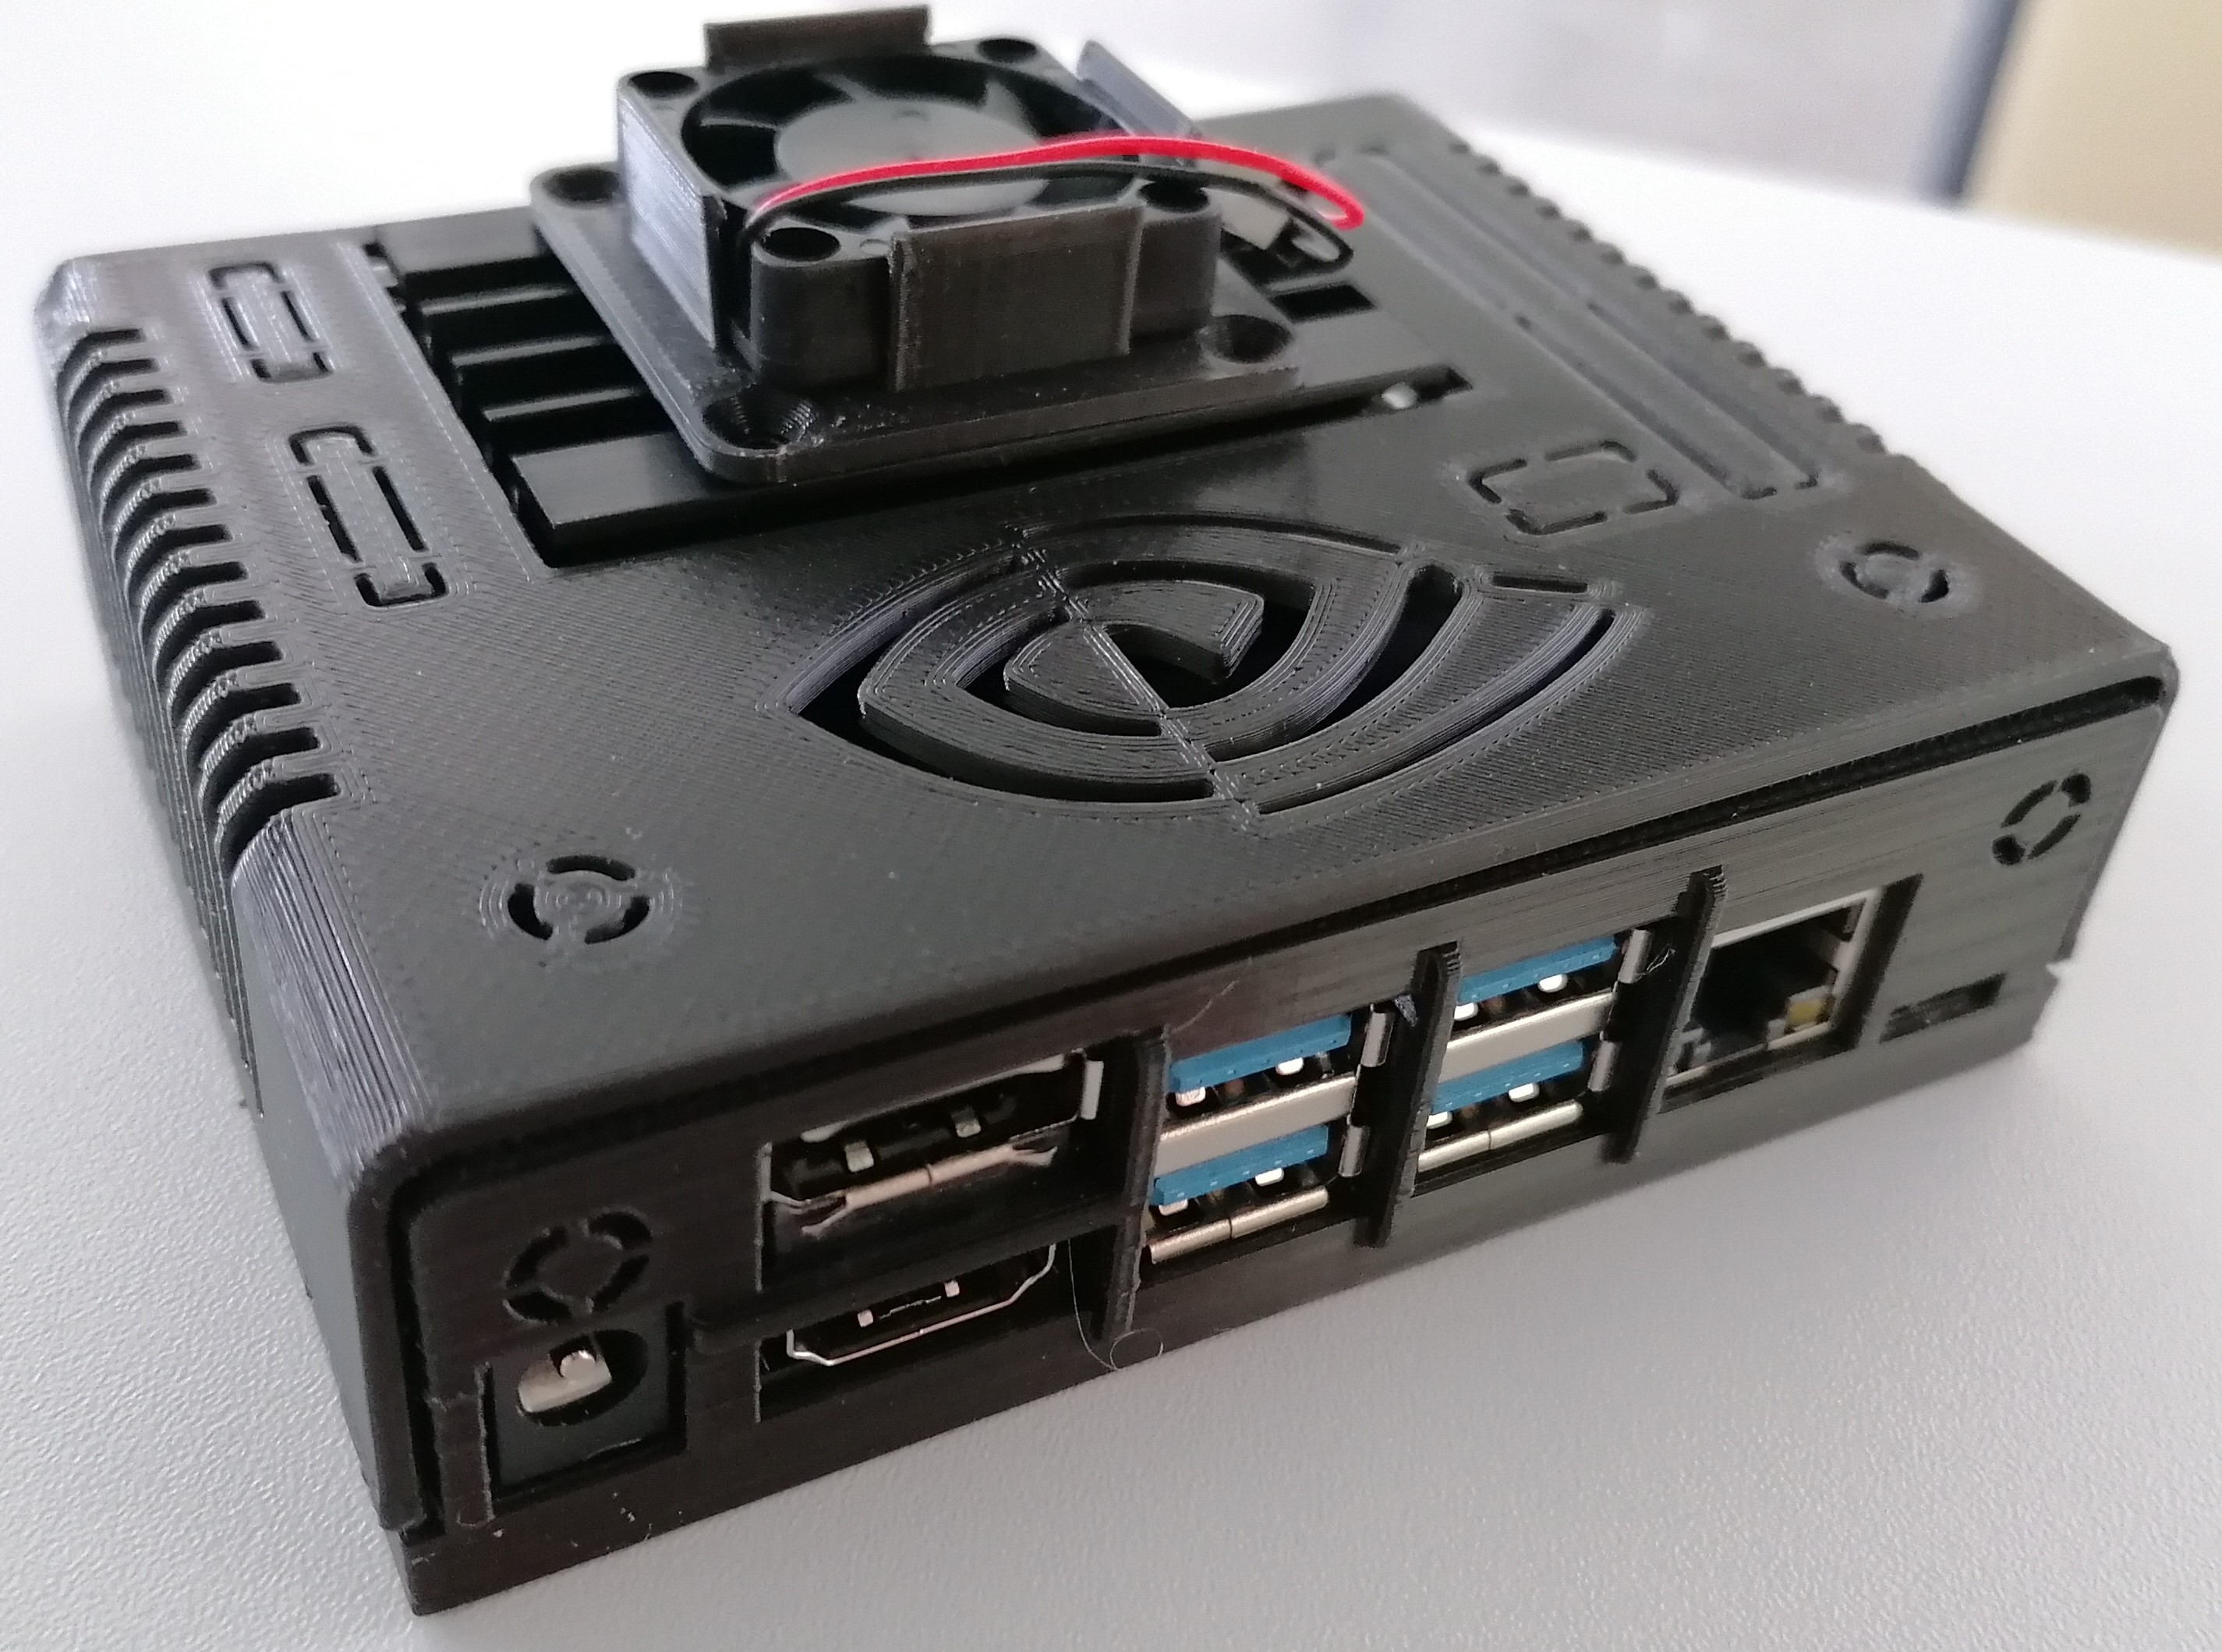
\includegraphics[width=0.8\textwidth]{img/Gerät Aufbau/Gehäuse_Jetson_2.jpeg.jpg}
  \centering
  \caption{Akkugehäuse und Bordhalterung}
  \label{fig:Akkugehäuse und Bordhalterung}
\end{figure}

\newpage

\textbf{Kamera Aufbau:} Die Halterung für die Kamera und die Ultraschallsensoren, die sich oben im Gerät befinden, ist auf die Lagerböcke geschraubt. Die Komponenten der Halterung sind 3D-gedruckt. Die Kamera ist von innen an die Halterung geschraubt und die Ultraschallsensoren sind gesteckt. Weiter sind oben an dieser Halterung der Startknopf, der NOTAUS-Schalter und vier LED`s angebracht. Auf der Rückseite der Halterung sind die zwei H-Brücken angeschraubt.

\begin{figure}[H]
  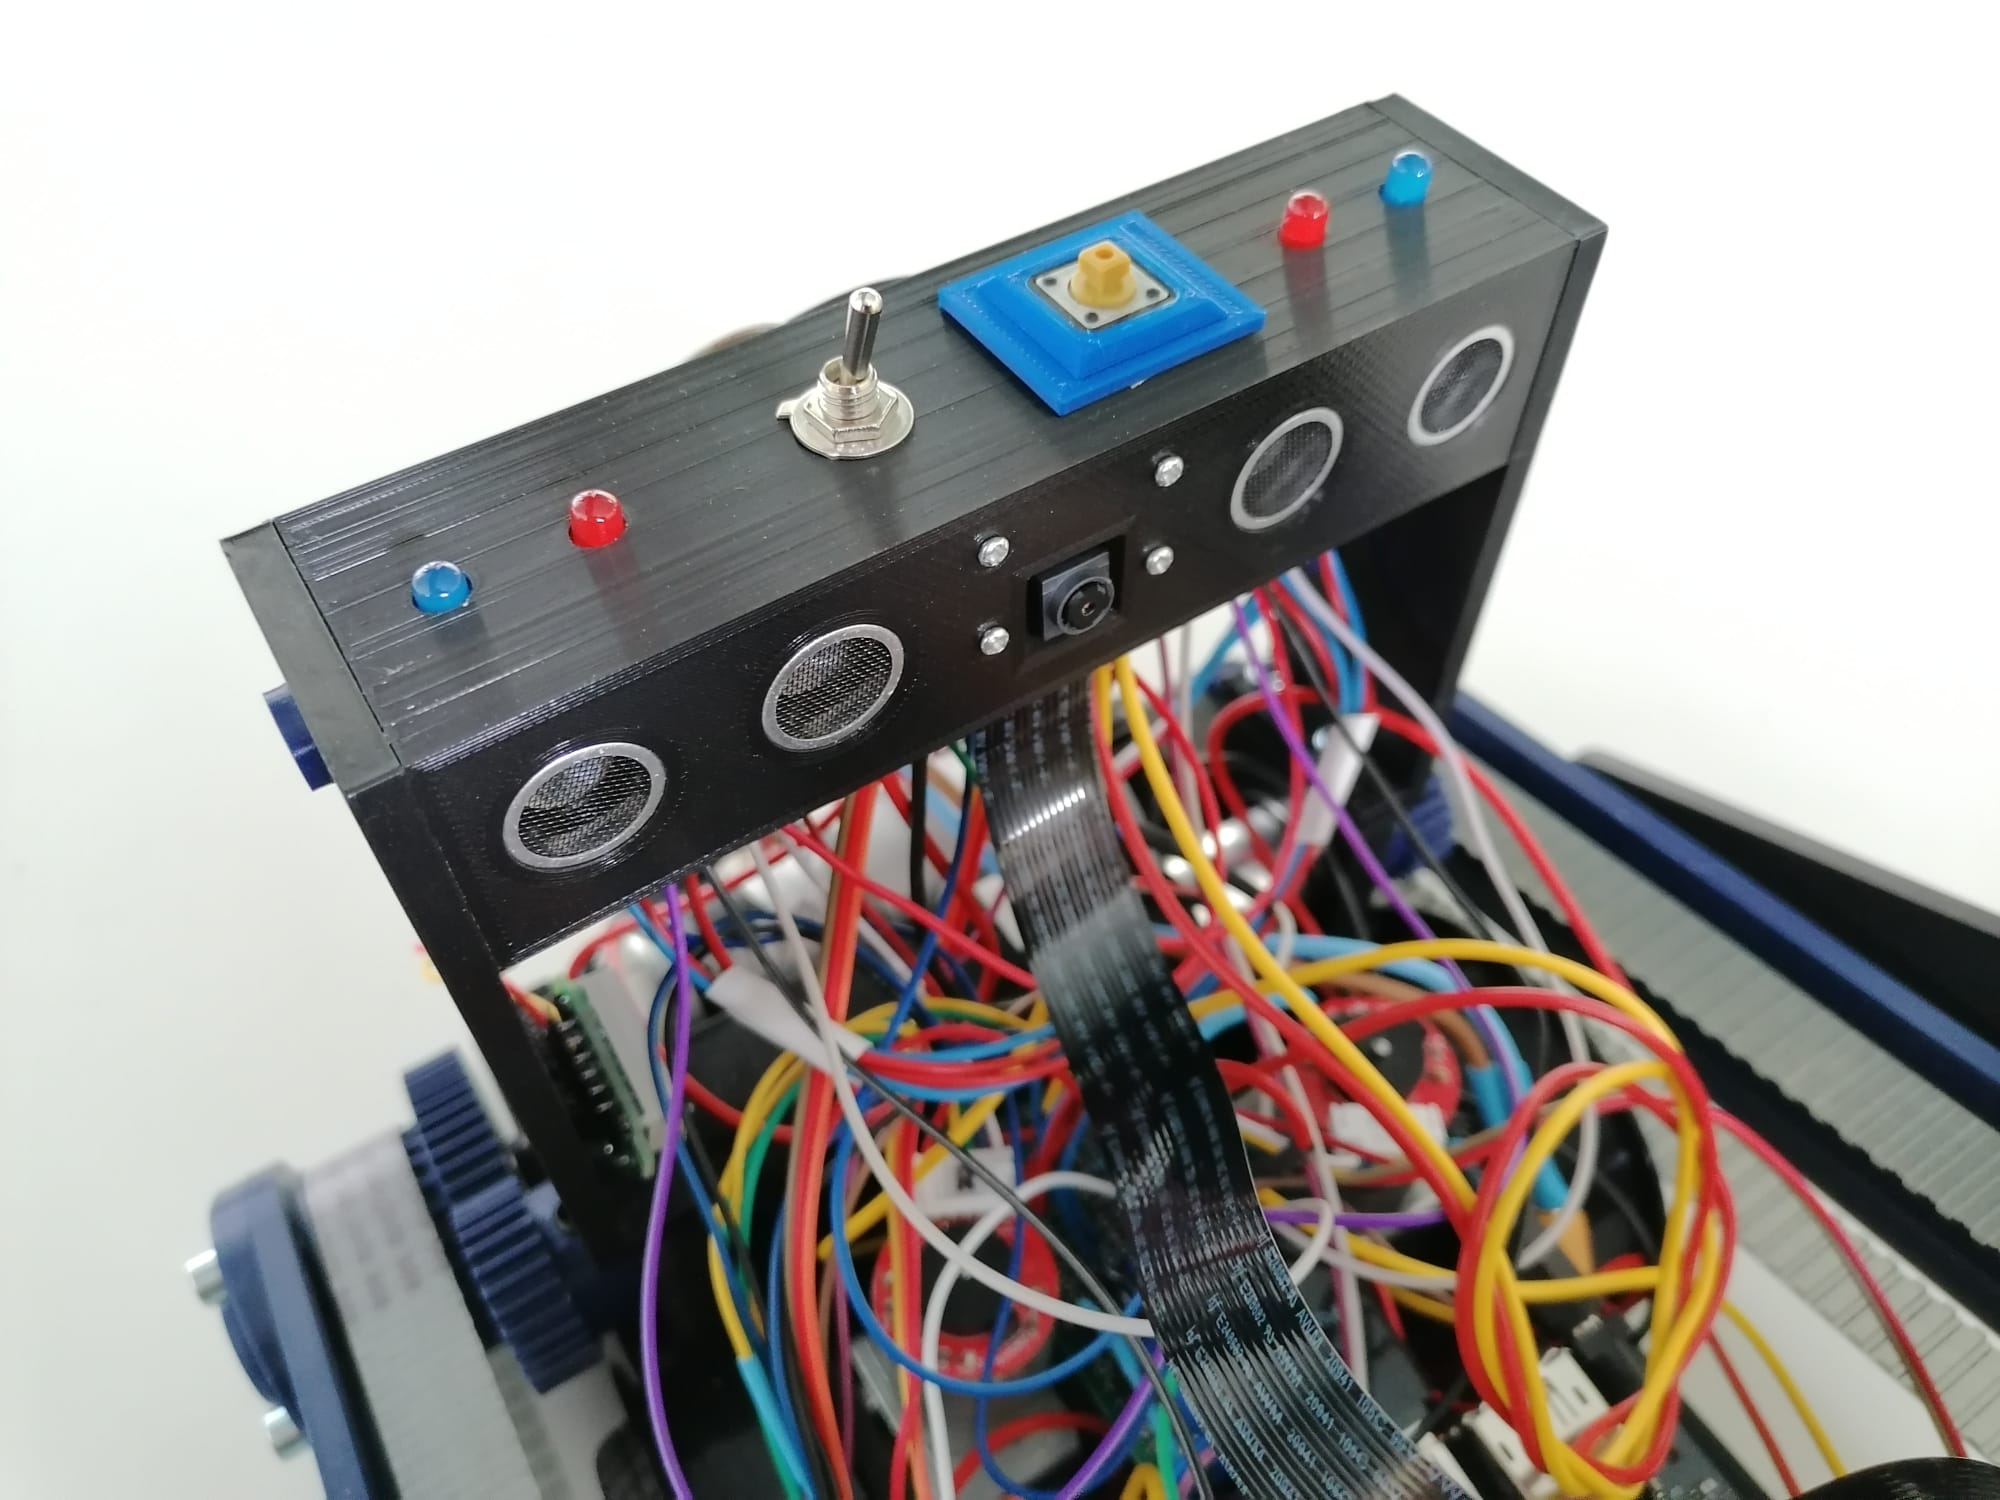
\includegraphics[width=0.65\textwidth]{img/Gerät Aufbau/KameraAufbau.JPG}
  \centering
  \caption{Kamera Aufbau}
  \label{fig:Kameraturnseite}
\end{figure}

\begin{figure}[H]
  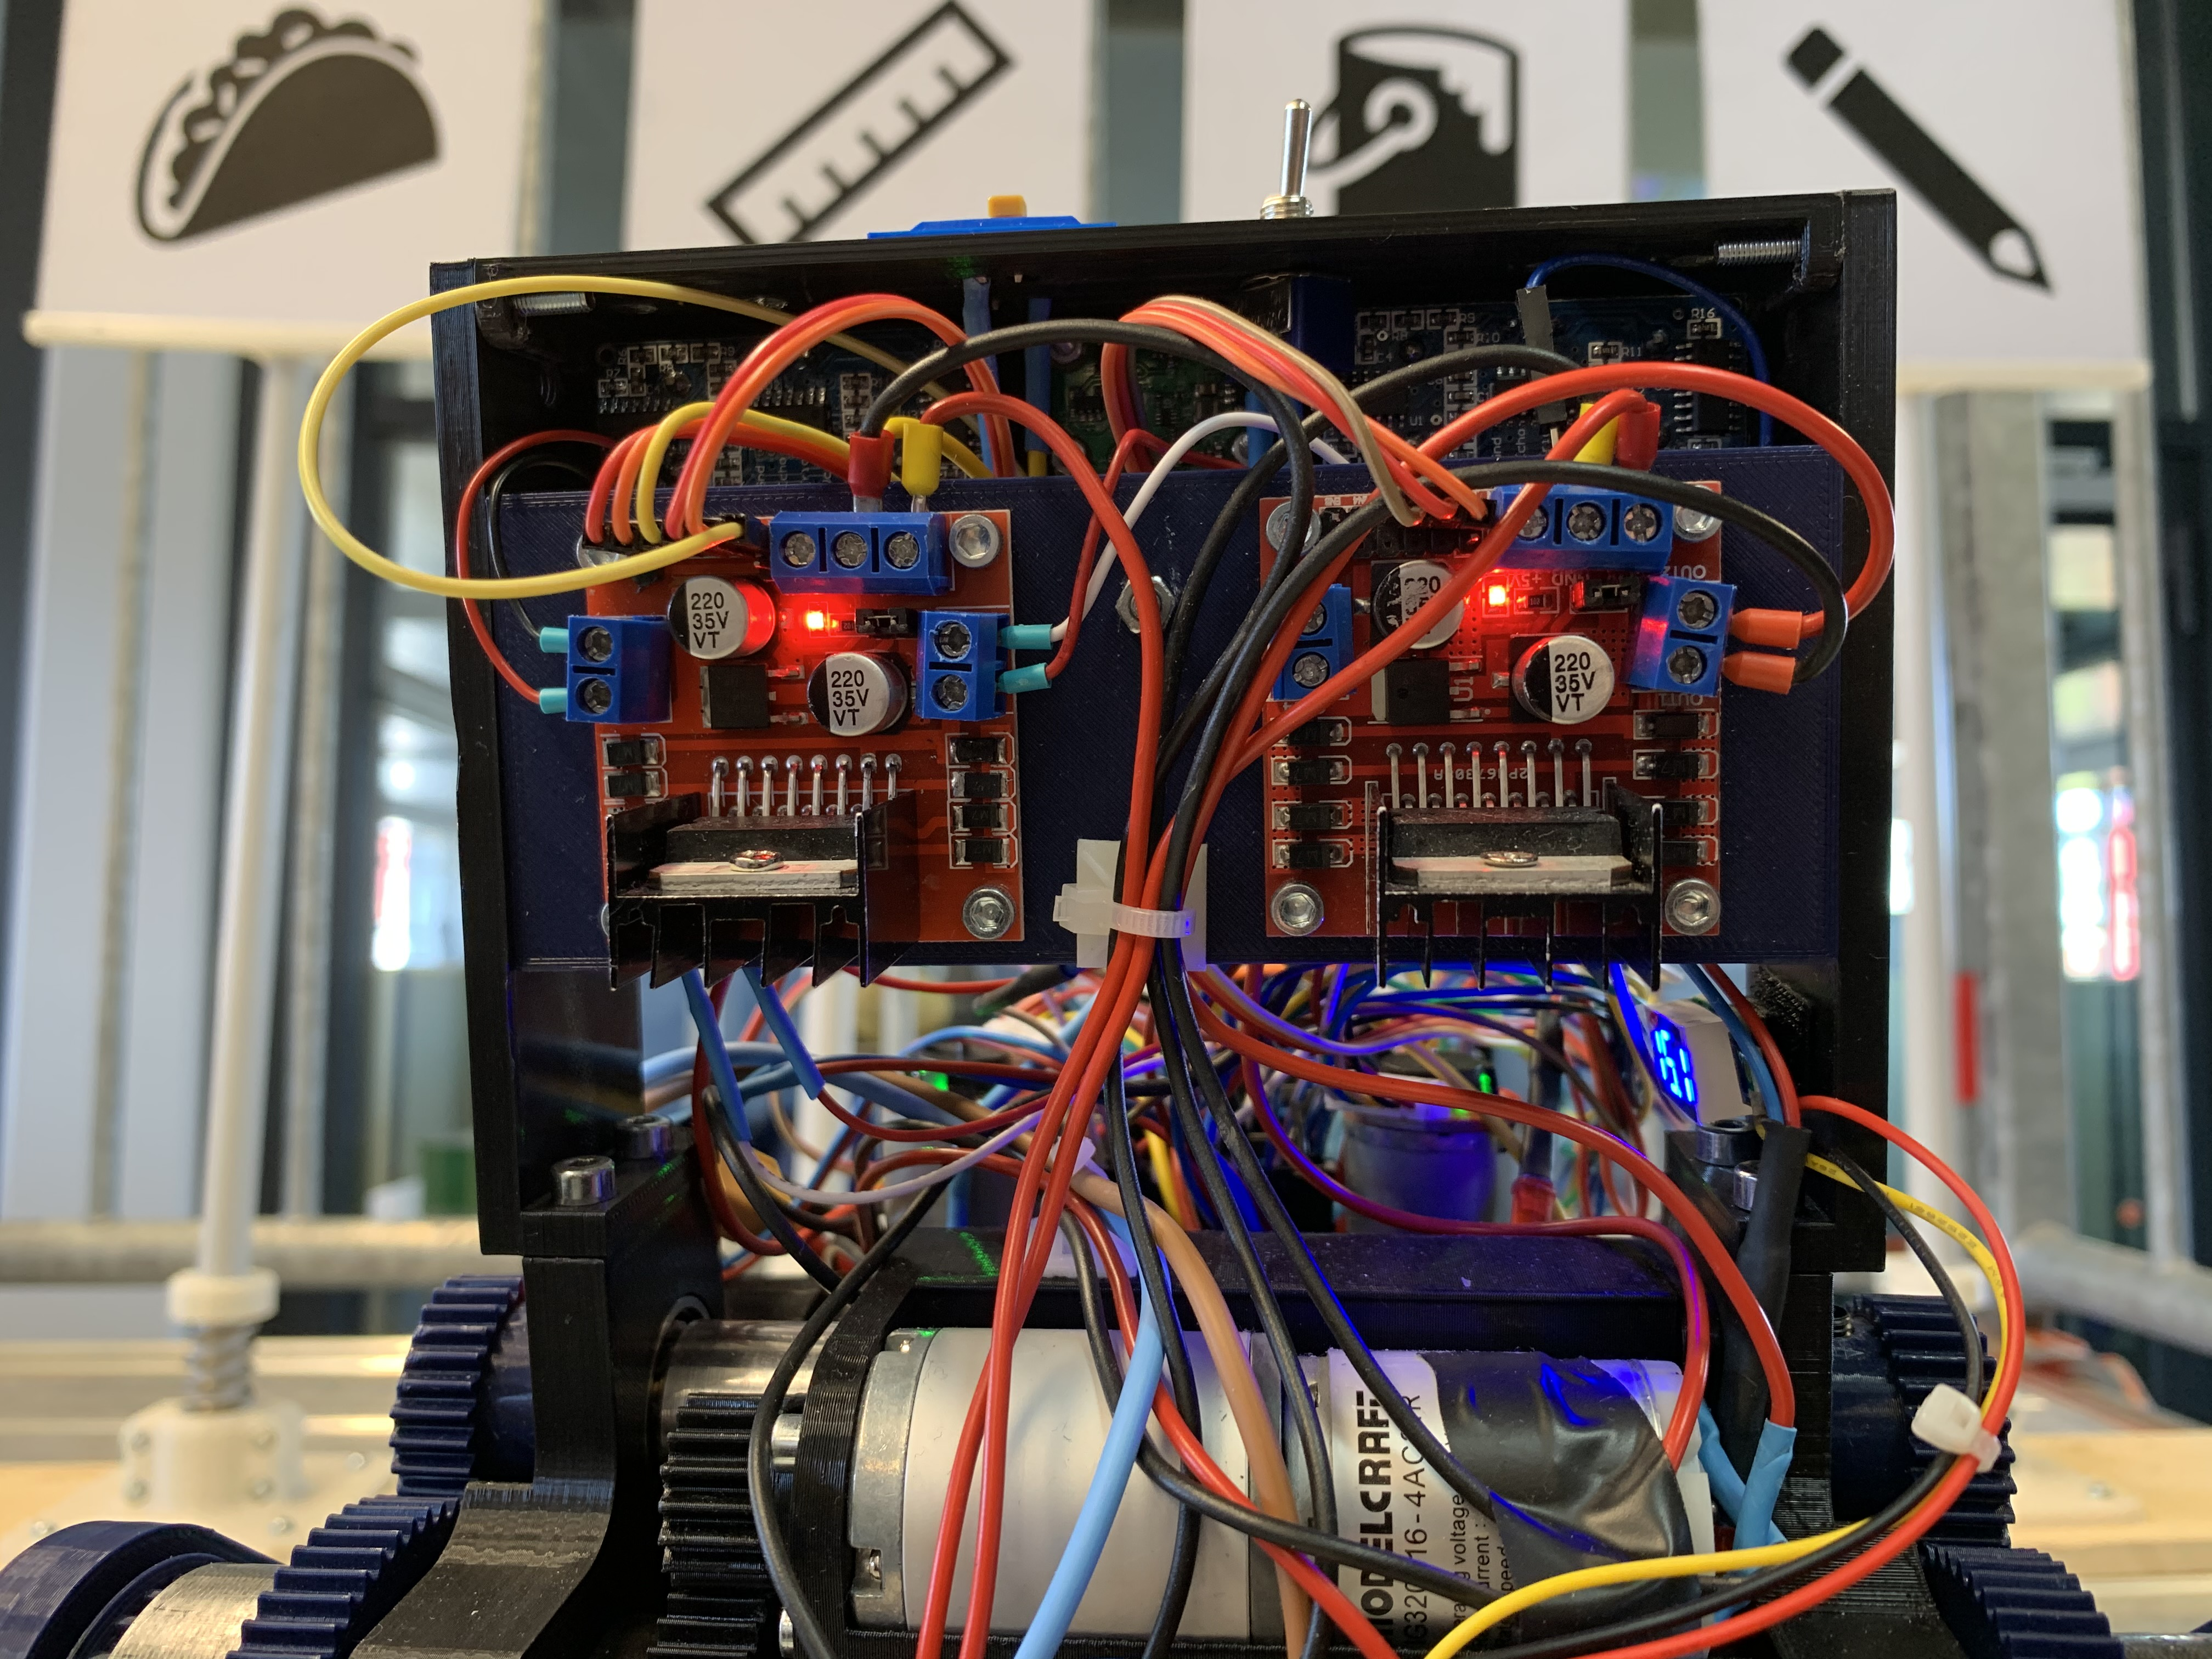
\includegraphics[width=0.65\textwidth]{img/Gerät Aufbau/KameraAufbau2.jpg}
  \centering
  \caption{H-Brücken an Kamera Aufbau}
  \label{fig:Kameraturmoben}
\end{figure}

\newpage

\textbf{Ultraschallsensorhalterung:} Der Ultraschallsensor, der sich vorne unten am Gerät befindet, ist in einer 3D-gedruckten Halterung an der Grundplatte angeschraubt.

\begin{figure}[H]
  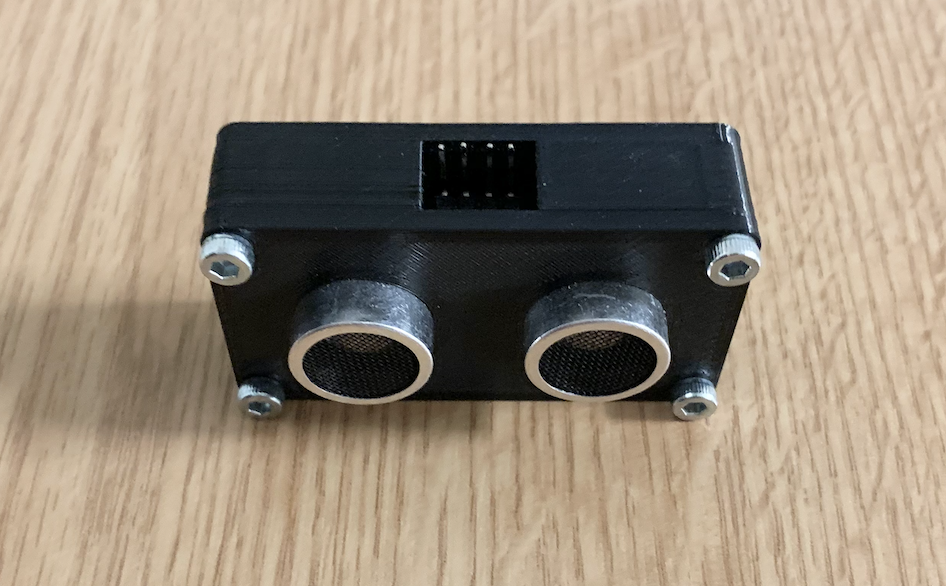
\includegraphics[width=0.6\textwidth]{img/Gerät Aufbau/Usensorhalterung.png}
  \centering
  \caption{Ultraschallsensorhalterung}
  \label{fig:Uschallsensorhalterung}
\end{figure}

\textbf{Halbkugelstützen:} Die Halbkugelstützen erfüllen zwei Funktionen. Auf der einen Seite halten sie den Roboter gerade während der Fortbewegung, auf der anderen Seite geben die Stützen, welche auf Tastern montiert sind, das Signal für den Bodenkontakt.

\begin{figure}[H]
  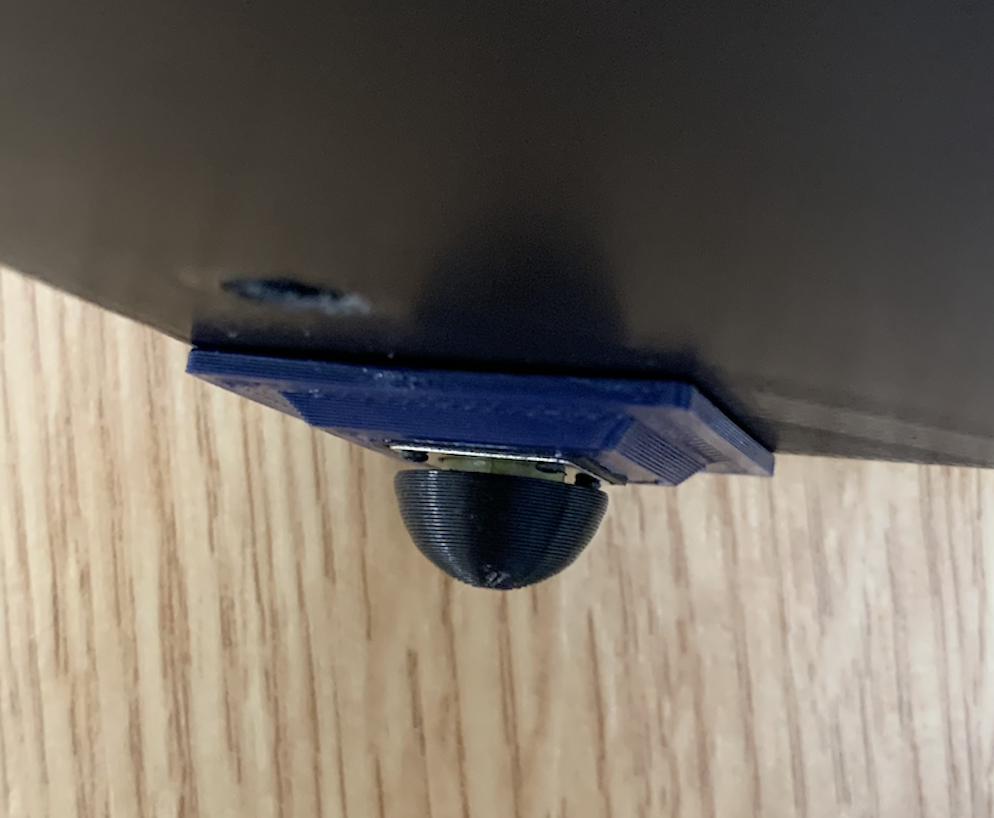
\includegraphics[width=0.6\textwidth]{img/Gerät Aufbau/Halbkugel.png}
  \centering
  \caption{Halbkugelstütze}
  \label{fig:Halbkugelstütze}
\end{figure}

\newpage

\textbf{Haube:}

Das Gerät wird von einer Haube geschützt. Diese Haube lässt sich von oben über den Grundkörper schieben und wird mit Schrauben an die Grundplatte geschraubt. Die Haube wurde aus mehreren 3D-gedruckten dünnen Platten zusammengeklebt. So konnte die Haube dünn und leicht gebaut werden.

\begin{figure}[H]
  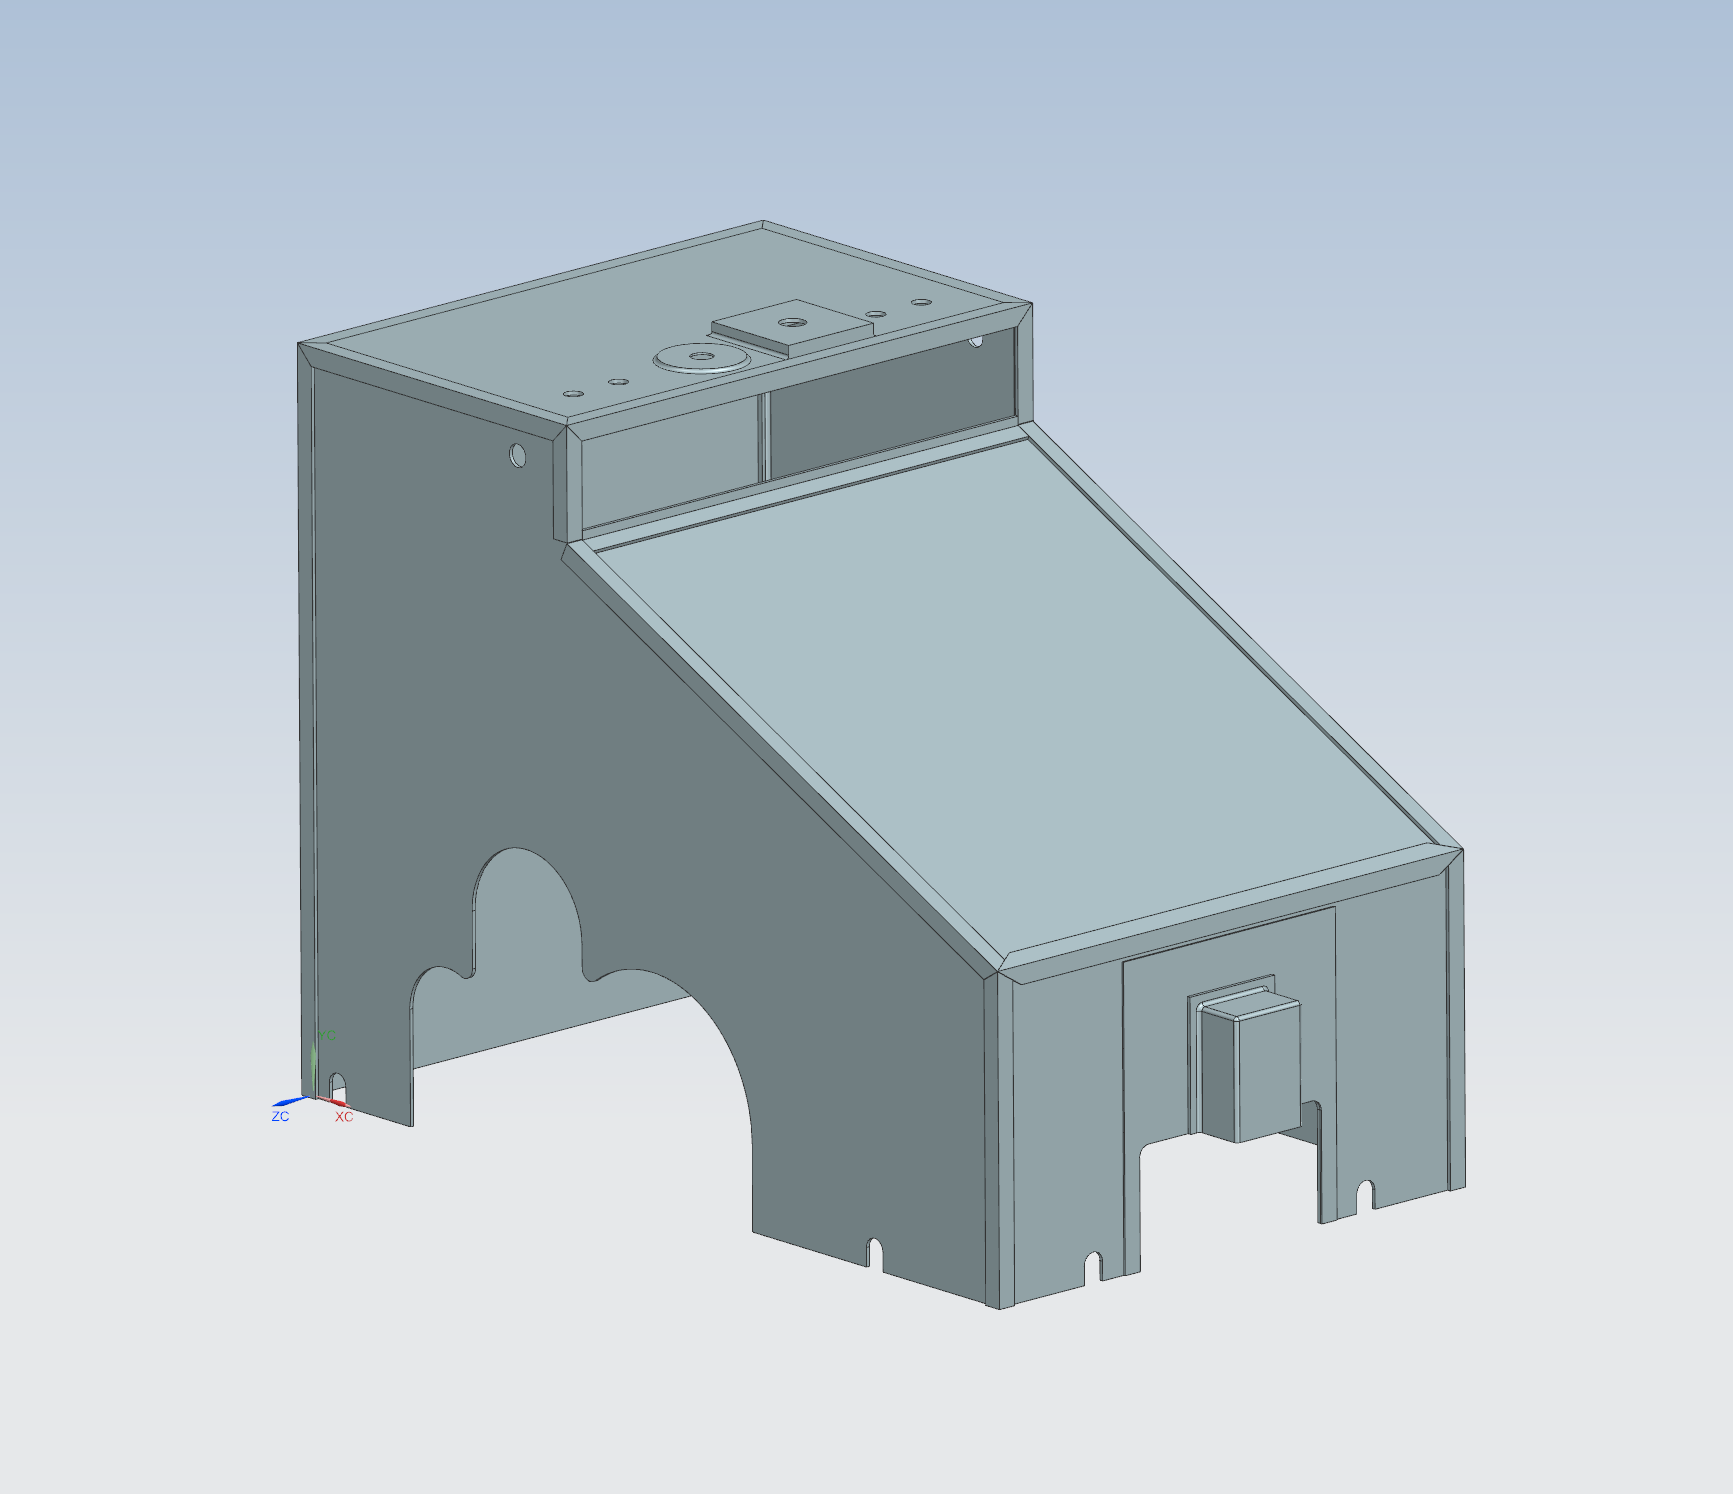
\includegraphics[width=0.8\textwidth]{img/Gerät Aufbau/CADHaube.PNG}
  \centering
  \caption{CAD-Entwurf der Haube}
  \label{fig:Haube}
\end{figure}

\begin{figure}[H]
  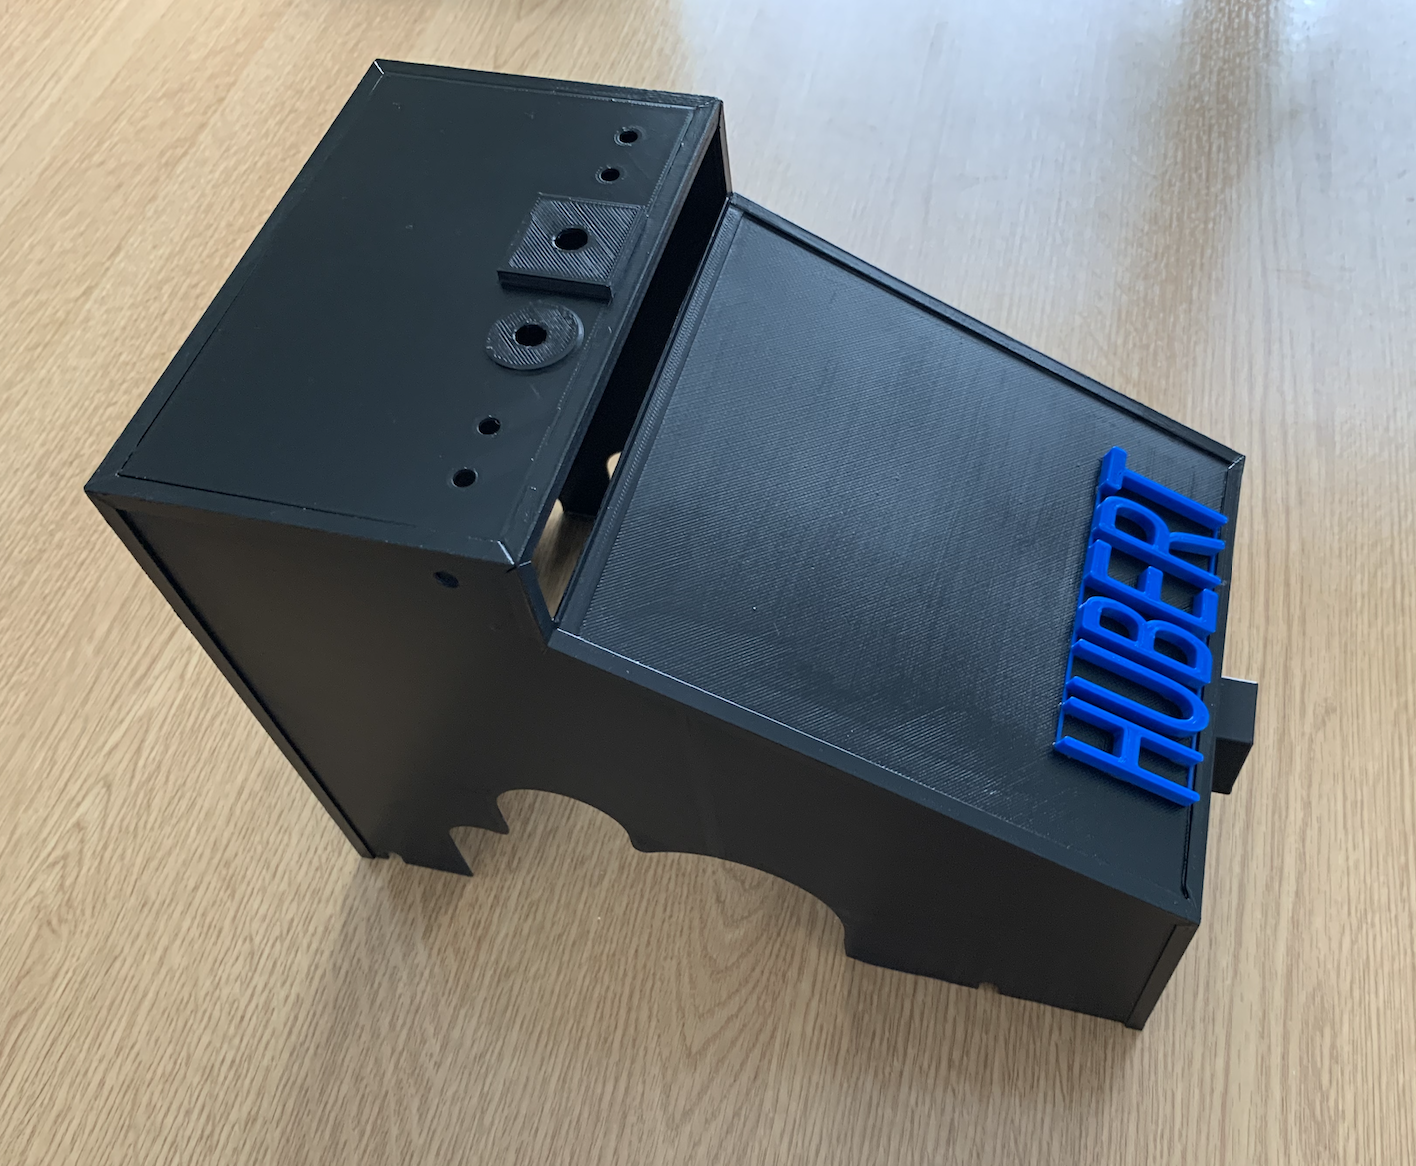
\includegraphics[width=0.8\textwidth]{img/Gerät Aufbau/Haube.png}
  \centering
  \caption{Haube des Grundkörpers}
  \label{fig:Haube1}
\end{figure}






\newpage

\subsection{Elektronikkomponenten}
\subsection{Pinbelegung}
Die Abbildung \ref{fig:pinout-jetson} zeigt die Pinbelegung des Jetson. Am Nvidia Jetson Nano sind folgende Komponenten angeschlossen:

\begin{itemize}
    \item ein \acrshort{i2c}-PWM-Board für die PWM-Signale zu den H-Brücken 
    \item drei Ultraschallsensoren
    \item zwei Taster für den Grundkörper und ein Starttaster
    \item zwei H-Brücken für Fortbewegung/Treppensteigen
    \item zwei Encoder für je ein Motor der Fortbewegung
    \item vier LEDs für Bestätigung
\end{itemize} 

\begin{figure}[H]
  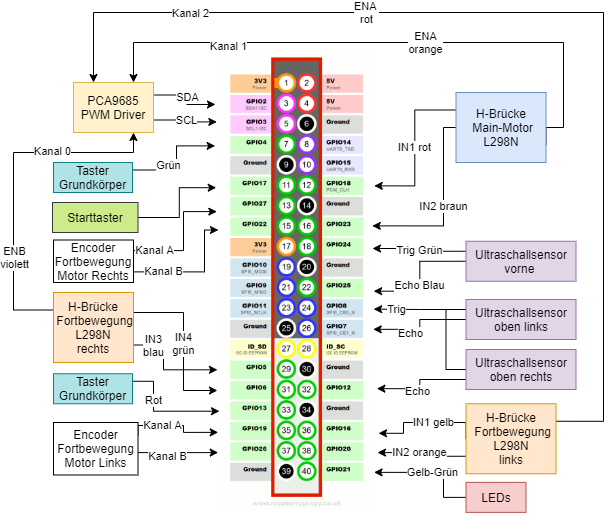
\includegraphics[width=0.8\textwidth]{img/Elektronik/pinout.png}
  \centering
  \caption{Pinbelegung des Jetson Nano}
  \label{fig:pinout-jetson}
\end{figure}


\newpage

\subsection{Taster}

Um zu erkennen, dass der Grundkörper auf der Treppe ist, werden zwei Mikrotaster verwendet, welche aktiv sind, sobald sie einen Untergrund berühren. Der erste Pin des Tasters ist mit einem GPIO-Pin des Jetson (Abb. \ref{fig:pinout-jetson}) und der zweite Pin ist mit Ground verbunden. Sobald der Taster aktiv ist, wird der GPIO-Pin des Jetson auf Ground gezogen. 

Der dritte Taster ist für das Startsignal verantwortlich. Dieser ist gleich angeschlossen, wie die Taster für den Grundkörper und startet den vorprogrammierten Bewegungsablauf.

\subsection{Motor für das Treppensteigen}
Der Motor für die Funktion des Treppensteigens wird an eine H-Brücke angeschlossen gemäss Abbildung \ref{fig:hbrücke-treppe}. Drei weitere Pin der H-Brücke sind mit dem Jetson verbunden. Die Leitung ENA oder ENB übertragen das PWM-Signal, welches die Geschwindigkeit der Motoren steuert. Die Leitungen IN1/IN2 steuern den Links- oder Rechtslauf des Motors. Sind beide Leitungen auf Low, sind die Motoren aus. Ist eine Leitung auf High und die andere auf Low, dreht der Motor links oder rechts herum.

\begin{figure}[H]
  \includegraphics[width=0.4\textwidth]{img/Elektronik/h_brücke_motoren_treppensteigen.png}
  \centering
  \caption{Anschluss der Motoren an die H-Brücke}
  \label{fig:hbrücke-treppe}
\end{figure}

\newpage

Dazu wurde ein GUI erstellt, um die Hubbewegung sowie die Drehung der Ausleger in einem ersten Versuch zu testen. Der linke Teil der Anzeige ist für die Ansteuerung des Hubmotors. Zu Beginn wird mit dem Schieberegler ein Duty Cycle beziehungsweise eine Geschwindigkeit des Motor eingestellt. Dieser Wert liegt zwischen 0 und 100. Danach kann durch Drücken auf den Button \glqq Links\grqq{} oder \glqq Rechts\grqq{} die Motordrehung gestartet werden. Der Motor dreht solange, bis auf den Button \glqq Stop\grqq{} gedrückt wird. Im unteren, linken Teil kann in der Spinbox die Frequenz des PWM-Signals für die H-Brücken eingestellt werden. Diese Frequenz wird auf 100 Hz gesetzt, da dies eine sinnvolle Frequenz für die H-Brücken ist. Der mittlere Teil gehört zum Motor der Ausleger und analog zum Bedienen des Hubmotors.
Der rechte Teil ist für die Fortbewegungsmotoren. Diese können durch das Drücken auf den \glqq Vorwärts-\grqq{} oder \glqq Rückwärts\grqq{}-Button angesteuert werden. Mit dem Button \glqq Turn\grqq{} wird eine Drehung ausgeführt. Dabei wird ein Motor etwas schneller vorwärts und der andere Motor etwas langsamer rückwärts angesteuert. Mit dem Button \glqq Stop\grqq{} werden beide Motoren gestoppt. Zum Schluss kann die Anwendung mit dem Button \glqq Exit\grqq{}, welcher unten in der Mitte ist, geschlossen werden. Wurden die Motoren nicht manuell gestoppt, werden beim Schliessen der Anwendung alle Motoren gestoppt.

\begin{figure}[H]
  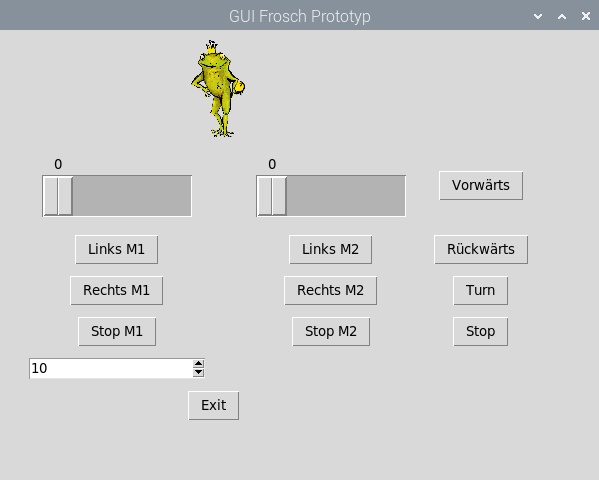
\includegraphics[width=0.6\textwidth]{img/Elektronik/gui_motoren.png}
  \centering
  \caption{GUI Motorensteuerung}
  \label{fig:gui-motoren}
\end{figure}

\newpage

\subsection{Motoren für Fortbewegung}
Für die Fortbewegung werden 12V DC Getriebemotoren mit Encoder und abgewinkelter Ausgangswelle gewählt \cite{Motoren-Fortbewegung}. Die Motoren werden gleich wie der Motor der Hubbewegung an eine weitere H-Brücke angeschlossen (Abb. \ref{fig:hbrücke-fortbeweg}).
Um zu Beginn, für erste Tests mit dem Roboter vorwärts und rückwärts fahren zu können, wurde im bereits erstellten GUI jeweils ein Button für vor-/rückwärts hinzugefügt.

\begin{figure}[H]
  \includegraphics[width=0.6\textwidth]{img/Elektronik/h_brücke_motoren_fortbewegung.png}
  \centering
  \caption{Anschluss der Motoren an die H-Brücke für Fortbewegung}
  \label{fig:hbrücke-fortbeweg}
\end{figure}

\subsubsection{Encoder}
Encoder oder auch Winkelmesser sind in der Lage, den vorangeschrittenen Winkel bei einer Drehung des Motors zu bestimmen. Mit dieser Winkelangabe und dem Umfang des Rades kann somit die theoretisch gefahrene Distanz bestimmt werden. Die Gefahr dabei ist, dass ein Durchdrehen des Rades in der Software fälschlicherweise als zurückgelegte Distanz aufgenommen werden kann, weshalb der Encoder nicht alleine für die Orientierung verwendet wird, sondern von den Ultraschallsensoren unterstützt wird.

\begin{figure}[h]
  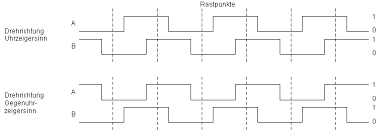
\includegraphics[width=0.7\textwidth]{img/Elektronik/quadrature.png}
  \centering
  \caption{Encoder Signal Kanal A und B}
  \label{fig:encoder-sig}
\end{figure}

Der Encoder gibt bei einer Umdrehung des Motors Rechteckpulse zurück. Durch das Zählen der Pulse vom Kanal A und B in einem fixierten Zeitintervall und der Anzahl der Pulse pro Umdrehung kann die Geschwindigkeit in Umdrehungen pro Minuten (rpm) wie folgt berechnet werden:

\begin{align*}
    Geschwindigkeit\ [rpm] = \frac{\frac{Encoder\ Ticks}{Ticks\ pro\ Umdrehung} \cdot 60\ s}{Zeitintervall\ [s]}
\end{align*}

Der Weg kann mittels Umfang des Rades ermittelt werden und in Anzahl Encoder Pulse umgerechnet werden.

\begin{align*}
    Anzahl\ Ticks = \frac{Distanz\ [cm]}{Umfang\ Rad\ [cm]} \cdot Ticks\ pro\ Umdrehung
\end{align*}

Für beispielsweise eine 90\textdegree-Drehung kann ein Rad vorwärts und das andere Rad rückwärts angesteuert werden, bis die benötigte Distanz erreicht wurde. 


\subsection{Ultraschallsensor}

Ultraschallsensoren sind gut, um ein breites Feld nach Gegenständen abzusuchen. Die Sensoren haben eine Ungenauigkeit von +-5mm, welche in Tests nachgewiesen werden konnte.
Im Roboter werden solche Sensor in Fahrtrichtung nach vorne verbaut. Die oberen Sensoren, welche neben der Kamera auf gleicher Höhe montiert werden, werden verwendet zur Bestimmung der Distanz und des Winkels zur Treppe. Der untere Sensor wird gebraucht, um die Kamera bei der Orientierung und vorallem dem Ausweichen von Hindernissen beim Traversieren auf der Treppe zu unterstützen.

Die Funktionsweise der Ultraschallsensoren kann wie folgt beschrieben werden:
Der Trigger des Sensors wird auf High gesetzt. Gleichzeitigt startet ein Timer auf dem Jetson. Mit dem Trigger wird ein Ultraschall ausgesendet. Sobald dieser zurückkehrt, wird dieses vom Sensor erkannt und ein High auf dem Echo an den Controller zurückgesendet. Mit diesem Signal wird der Timer gestoppt und aus der resultierenden Zeit kann mithilfe der Konstante zur Schallgeschwindigkeit die Distanz bestimmt werden.

Die Distanz kann durch folgende Formel berechnet werden:
\begin{align*}
    Distanz\ [m] = \frac{Zeit\ [s] \cdot 34300\ [\frac{cm}{s}]}{2}
\end{align*}
Die gemessene Zeit wird mit der Schallgeschwindigkeit multipliziert und durch zwei geteilt, da die Ultraschallwellen hin und zurück ausgebreitet hat. 
Das 5 Volt Echo-Signal, welches vom Sensor zurück zum Controller geht muss zudem durch einen Spannungsteiler mit drei Widerständen auf 3.3 V begrenzt werden, da die Pins des Jetson Nano nur bis maximal 3.3 V ausgelegt sind. Übersteigt die Eingangsspannung des Pins diese 3.3 V kann das Jetson Nano beschädigt werden.

\newpage

\subsection{Akku}
Im \acrshort{pren1} wurde bereits eine theoretische Berechnung für die Auslegung des Akkus gemacht. Um eine höhere Genauigkeit für die Kapazität zu erzielen, werden die elektronischen Komponenten beispielsweise die Motoren angesteuert und der Stromverbrauch mittels Multimeter gemessen:
\begin{itemize}
    \item Hauptmotor Hubbewegung: 0.65 A
    \item Hilfsmotor Hubbewegung: 0.35 A
    \item Motoren Fortbewegung: 2 \cdot\ 0.25 A
    \item Jetson Nano: 0.9 A
\end{itemize}
Daraus folgt 
\[C = {I\cdot t} = \frac{2.4\ A\cdot 12\ min}{60} \cdot 1000 = 480\ mAh\]
Mit Faktor 4 als Reserve ergibt sich ein Modellbauakku mit ungefähr 2300 mAh von Tattu \cite{Akku-Modellbau}. Diese Kapazität wurde gewählt, damit der Roboter auch für längere Zeit mit Strom versorgt wird. Dies ist von Vorteil beim Entwickeln und Testen des Roboters. Dadurch können mehrere Testläufe hintereinander durchführt werden, ohne den Akku immer wieder laden zu müssen.

Ergänzend zu erwähnen ist, dass diese Berechnung vor dem Entfernen des zweiten Hubbewegungsmotors gemacht wurde, wodurch die bereits vorhandene Reserve erweitert wird.

\newpage

\newpage
\subsection{Schema}
\begin{figure}[h]
  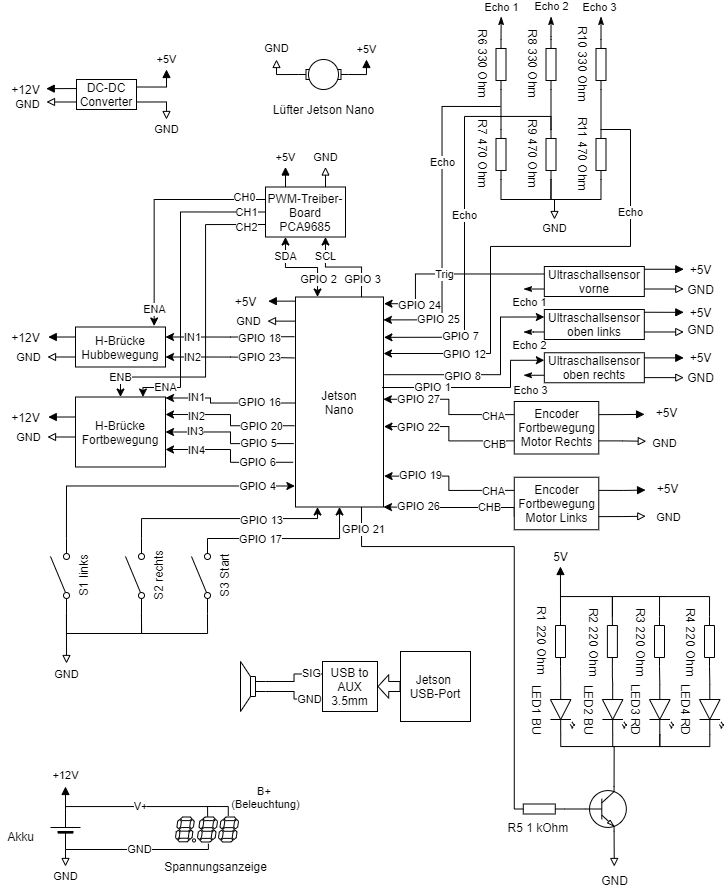
\includegraphics[width=0.8\textwidth]{img/Elektronik/schema.png}
  \centering
  \caption{Schema der Elektronikkomponenten des Roboters}
  \label{fig:schema}
\end{figure}

\newpage

Nachfolgend werden die Elektronikkomponenten, welche noch nicht näher erläutert wurden, kurz beschrieben.\\

\textbf{DC-DC-Converter:} Der DC-DC-Converter wandelt eine Eingangsspannung von ungefähr 13 V - 16.6 V in eine konstante Spannungsversorgung von 5 V für beispielsweise das Jetson Nano und die verschiedenen Sensoren. Dieser wurde gewählt, da er kostengünstig ist, eine Eigenentwicklung zu viel Zeit beansprucht hätte und der eingekaufte Wandler über eine nachweisbare Langlebigkeit und Qualität verfügt. Die Ausgangsspannung kann mittels Potentiometer eingestellt werden. Diese wird auf ca. 5.1 V eingestellt, damit, falls die Belastung steigt und die Spannung leicht einbricht, immer mindestens 5 V anliegen.\footnote{\url{https://www.conrad.ch/de/p/makerfactory-spannungsregler-mf-6402402-1-st-2134134.html?searchType=SearchRedirect}}\\

\textbf{Spannungsanzeige:}\footnote{\url{https://www.lightinthebox.com/de/p/mini-dc-0-100-v-3-digital-voltmeter-rot-led-led-spannungsanzeige-meter-3-draehte_p7931743.html?currency=CHF&litb_from=paid_adwords_shopping&sku=1_16&country_code=ch}} Die Spannungsanzeige ist eine 7-Segmentanzeige mit drei Ziffern. Diese Anzeige ist am Akku angeschlossen damit kann der Ladezustand des Akkus überprüft und einer Tiefenentladung vorgebeugt werden. Fällt die Spannung unter 13 V sollte der Akku aufgeladen werden.\\

\textbf{Akku:} Der Akku \cite{Akku-Modellbau} ist ein vier Zellen LiPo-Akku mit einer Kapazität von 2300 mAh. Dieser versorgt die Bauteile des Robotors mit Spannung. Ist der Akku voll geladen, liefert er eine Spannung von ungefähr 16.6 V. Die Spannung einer einzelnen Zelle sollte nie unter 3 Volt fallen. Der Akku hat somit eine untere Spannungsgrenze von 12 Volt welche nicht unterschritten werden sollte um Kapazitätsverlust zu verhindern.\\

\textbf{LED:}\footnote{\url{https://www.distrelec.ch/de/led-rot-mm-no-brand-led-rd-dif/p/17510241?track=true&no-cache=true&marketingPopup=false}} Die LED's haben die Aufgabe, das Erkennen des Piktogramms zu signalisieren. Die vier LED's werden gleichzeitig durch das Jetson Nano über einen NPN-Transistor, welcher als Schalter dient, angesteuert. Die Spannung über den LED's wird über die Vorwiderstände eingestellt und der Widerstand an der Basis des Transistors begrenzt den Strom zwischen Transistor und Ausgang des Jetson Nano.\\

\textbf{PWM-Treiber}: Das PWM-Treiber-Board \footnote{\url{https://www.bastelgarage.ch/16-kanal-pwm-servo-treiber-i2c-pca9685?search=420049}} generiert durch den PCA9685 Controller PWM-Signale, welche für die H-Brücken der Motoren zur Steuerung der Geschwindigkeit benötigt werden. Die Befehle für beispielsweise den Duty-Cylce eines PWM-Signals wird vom Jetson Nano mittels \acrshort{i2c} auf den Controller übertragen. Dieses wurde gewählt, weil das Jetson Nano Board nur zwei Hardware-PWM-Ausgänge hat. Benötigt werden jedoch drei (zwei Fortbewegungsmotoren und ein Hubmotor). \\

\textbf{Lautsprecher}:\footnote{\url{https://www.digitec.ch/de/s1/product/x-mini-happy-capsule-mini-12h-bluetooth-portable-lautsprecher-281638}} Der Lautsprecher wird über eine USB-Soundkarte mit dem Jetson Nano verbunden. Dies, da das Jetson über keine interne Soundkarte verfügt. Der generische Mini-Lautsprecher wurde für einen symbolischen Beitrag von einem Teammitglied übernommen.


\newpage

\section{Standsicherheit beim Erklimmen einer Stufe}

Beim Erklimmen einer Stufe ist der kritische Fall, wenn sich die Ausleger horizontal auf einer Linie mit dem Grundkörper befinden. Wenn der Grundkörper auf die nächste Stufe gehoben wird befindet sich die Drehachse der Ausleger am Grundkörper 8 mm hinter der Kante der Stufe (siehe Abbildung \ref{fig:Erklimmen}).

\begin{figure}[h]
  \includegraphics[width=\textwidth]{img/Gerät Aufbau/Standsicherheit.png}
  \centering
  \caption{Gerät beim Erklimmen einer Stufe}
  \label{fig:Erklimmen}
\end{figure}

Um die Standsicherheit in diesem Fall berechnen zu können, wurde das Gewicht des Grundkörpers und der verbundenen Ausleger einzeln gewogen und der Schwerpunkt ermittelt.\\

Gewicht Grundkörper: $m_{GK}$ = 2.85 kg

Gewicht Ausleger: $m_{A}$ = 0.44 kg\\

Abstand Schwerpunkt Grundkörper zur Drehachse (Welle 1): $l_{1}$ = 52 mm

Abstand Schwerpunkt Ausleger zur Drehachse (Welle 1): $l_{2}$ = 190 mm

\newpage

\begin{align*}
M_{Kipp} = m_{A} \cdot g \cdot (l_{2}+8 mm) = 0.44\ kg \cdot 9.81\ \frac{m}{s^2} \cdot 0.198\ m = 0.85\ Nm
\end{align*}

\begin{align*}
M_{Stand} = m_{GK} \cdot g \cdot (l_{1}-8 mm) = 2.85\ kg \cdot 9.81\ \frac{m}{s^2} \cdot 0.044\ m = 1.23\ Nm
\end{align*}\\

Daraus folgt: $M_{Stand}$ > $M_{Kipp}$

\begin{align*}
Standsicherheit = \frac{M_{Stand}}{M_{Kipp}} = \frac{1.23\ Nm}{0.85\ Nm} = \underline{\underline{1.45}}
\end{align*}

Zusätzlich ist an die Unterseite des Grundkörpers Schleifpapier geklebt, um zu verhindern, dass das Gerät auf der Kante nach hinten rutscht.


\newpage

\section{Testing}

In diesem Abschnitt ist beschrieben, wie das das Konzept umgesetzt und verbessert wurde. Änderungen, welche während dem Bauen und Testen gemacht wurden, sind hier chronologisch festgehalten. 

\subsection{Manuelles Testing}
Für die allerersten Tests der Motorenansteuerung, wurde das GUI zur Hilfe genommen, welches in \acrshort{pren1} entwickelt wurde.

\textbf{Hubbewegung:}

Um den ersten Sprint erfolgreich abzuschliessen, wurden alle Teile, welche bereits in \acrshort{pren1} konstruiert wurden, mit den 3D-Druckern im Team produziert. Die Elektromotoren, welche für die Hubbewegung zuständig sind, wurden verbaut, ebenso die Motoren für die Fortbewegung um das Gewicht realistischer zu simulieren. Somit konnten die Hubbewegungen getestet werden und das 3D-Konstrukt auf Schwachstellen untersucht werden.

\begin{figure}[H]
  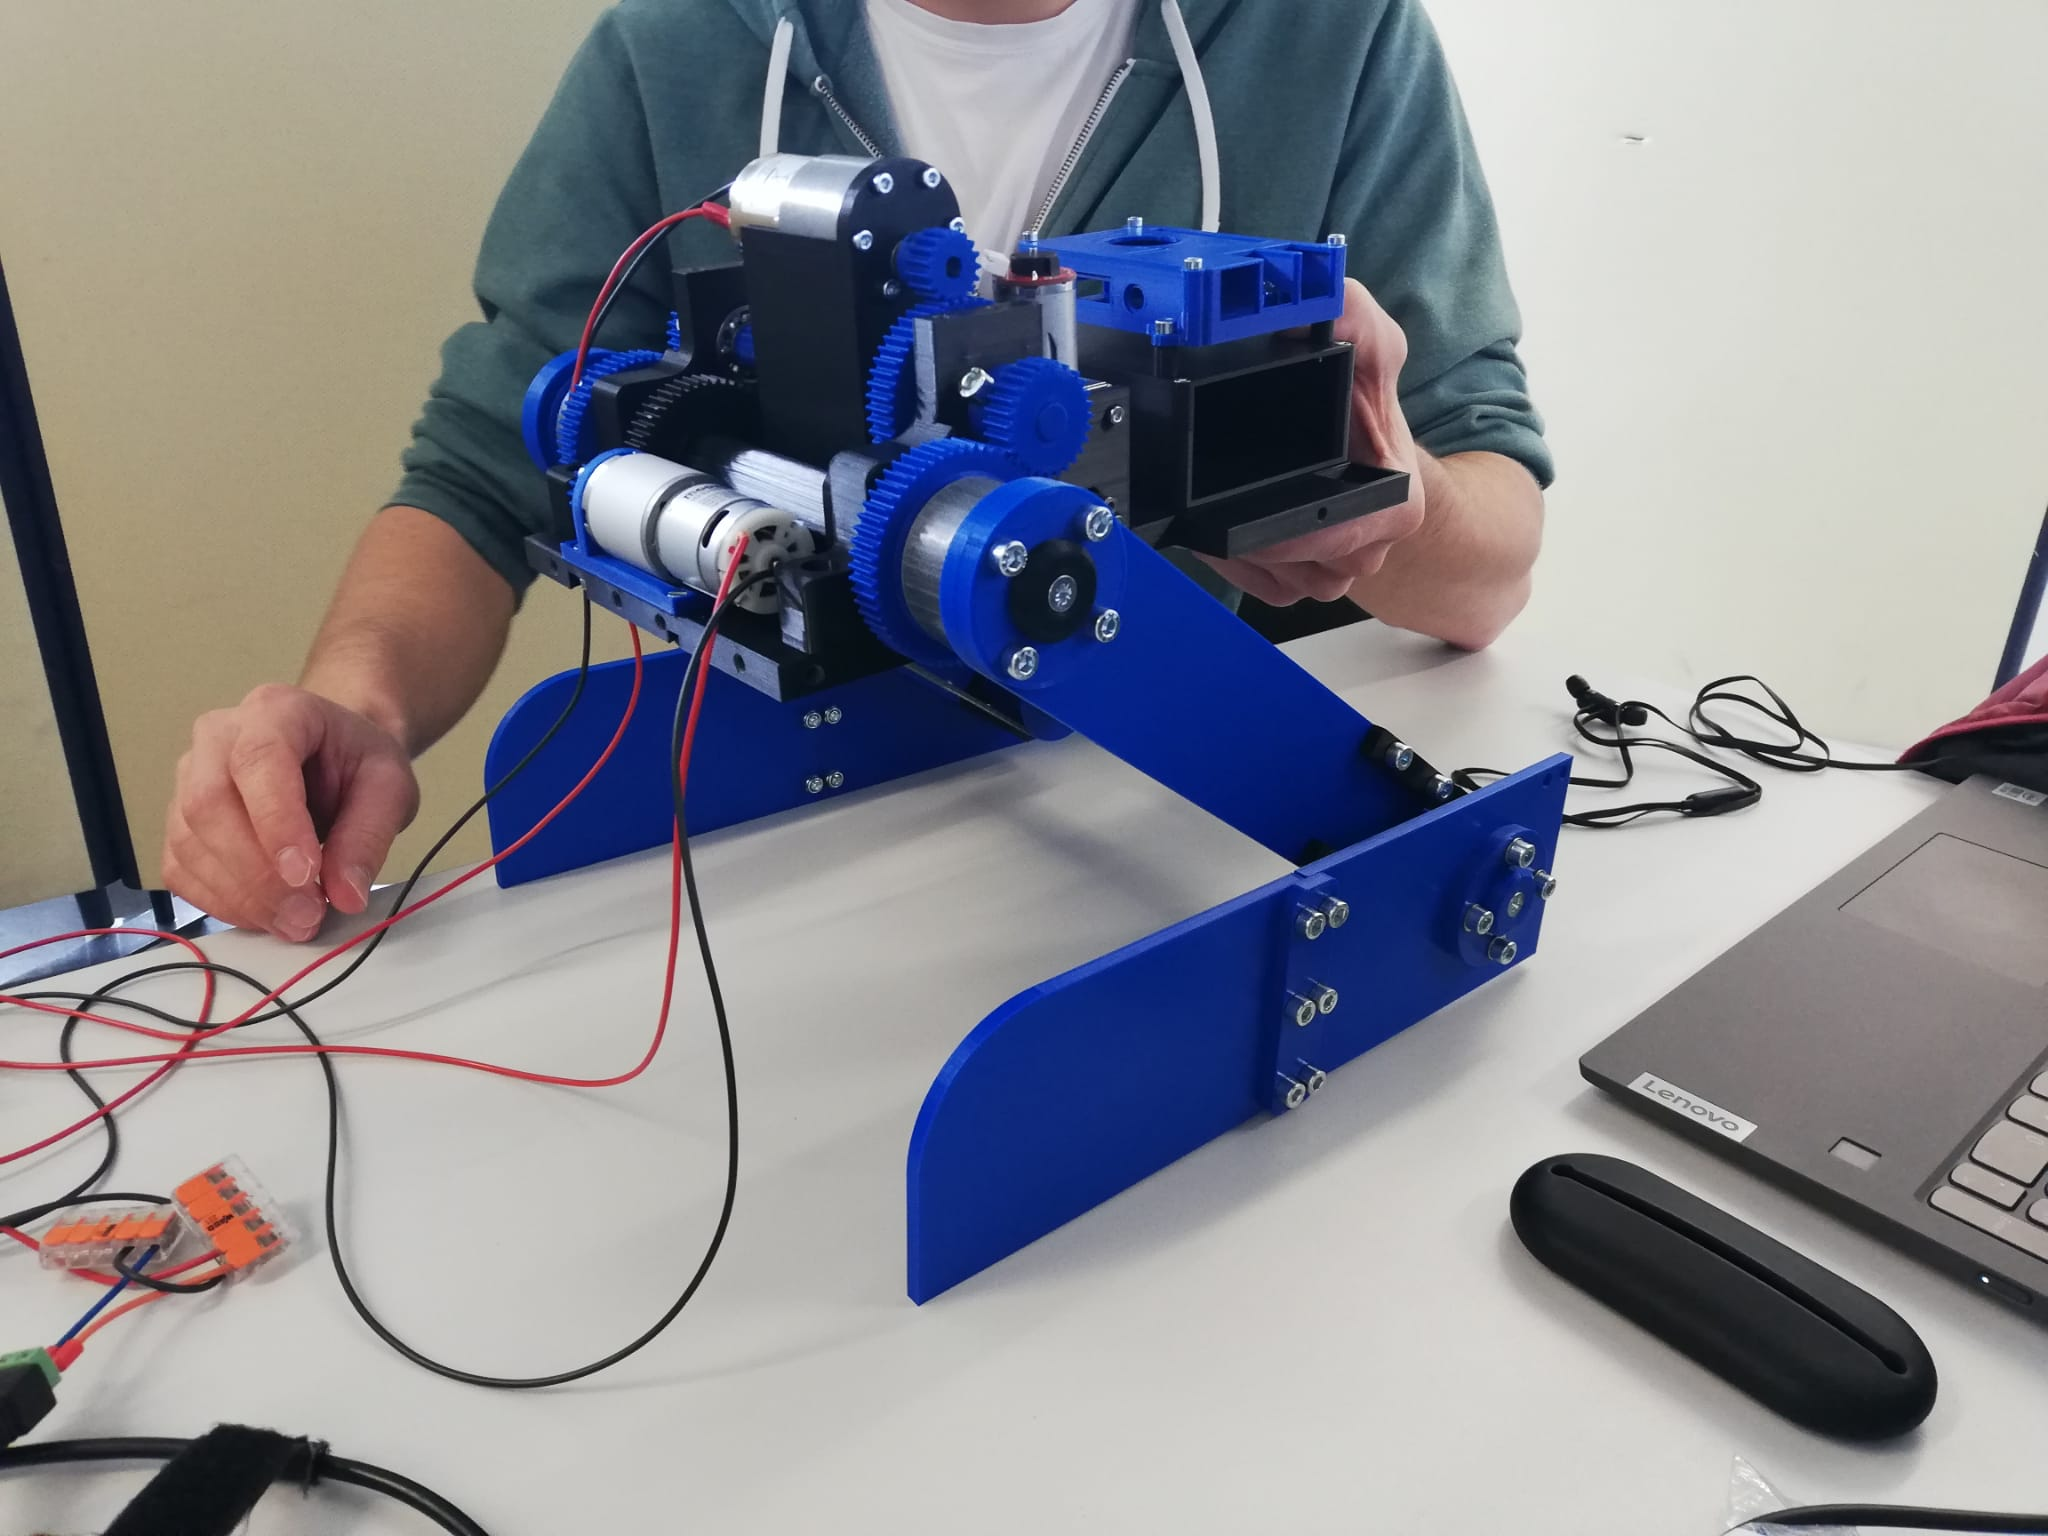
\includegraphics[width=0.7\textwidth]{img/Sprint1/pren1_sprint1_1.png}
  \centering
  \caption{Sprint 1 - Erste Prototypentests}
  \label{fig:erstePrototypentests}
\end{figure}

\newpage

In diesem Test offenbarte sich eine Schwachstelle. Das Motorritzel des Hubmotors konnte die Drehbewegung des Motors nicht aufnehmen, was zu einem Durchdrehen des Motors geführt hat.
Diese Schwachstelle des ersten Prototypen konnte schnell verbessert  werden, was zu einem schnellen, erfolgreichen zweiten Versuch führte.

\begin{figure}[H]
  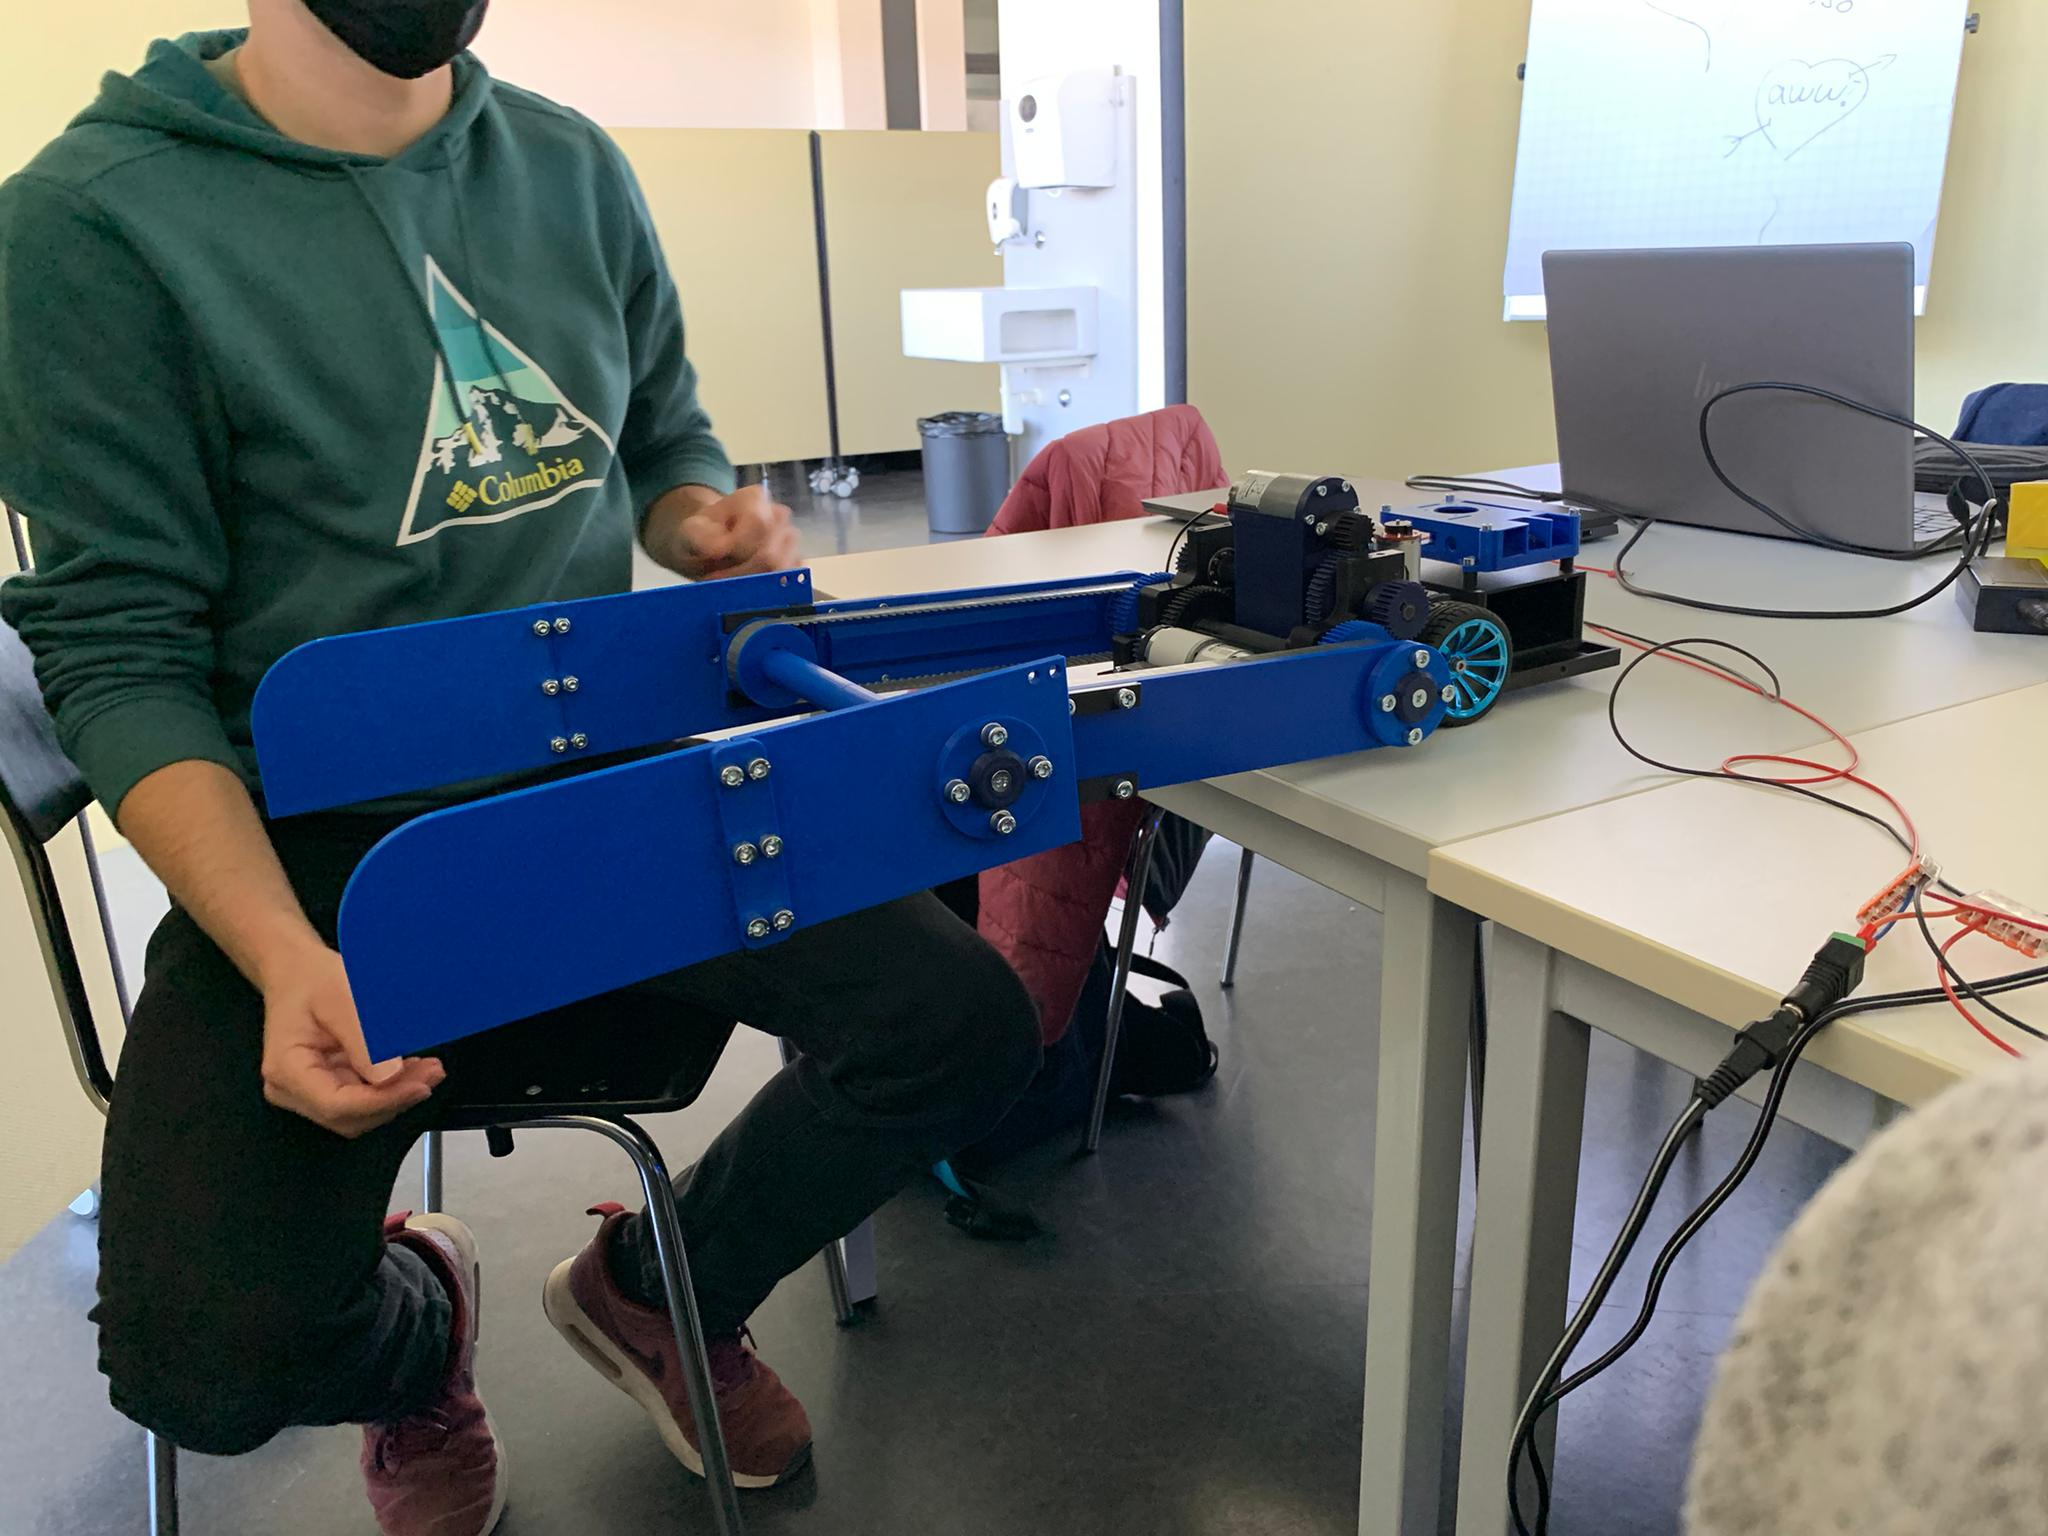
\includegraphics[width=0.7\textwidth]{img/Sprint1/pren1_sprint1_2.png}
  \centering
  \caption{Sprint 1 - Zweite Tests}
  \label{fig:zweiteTests}
\end{figure}

Mit den Verbesserungen war es möglich, die Erste und die zweite Hubbewegung ohne Überbelastung einzelner Teile durchzuführen.
Die volle Drehbarkeit der Ausleger wird nur noch von den Stromkabeln an den Motoren eingeschränkt. In einem zweiten Test wurden wiederum neu angekommene Teile direkt verbaut um langsam an das Zielgewicht heranzukommen.

Mit diesem Roboter konnten auch die ersten Versuche auf einer Treppe durchgeführt werden (siehe Abbildung \ref{fig:ersteTreppentests}). Dazu wurde der Roboter in verschiedenen Positionen auf der Treppe platziert und die erste Hubbewegung ausgeführt.

\begin{figure}[H]
  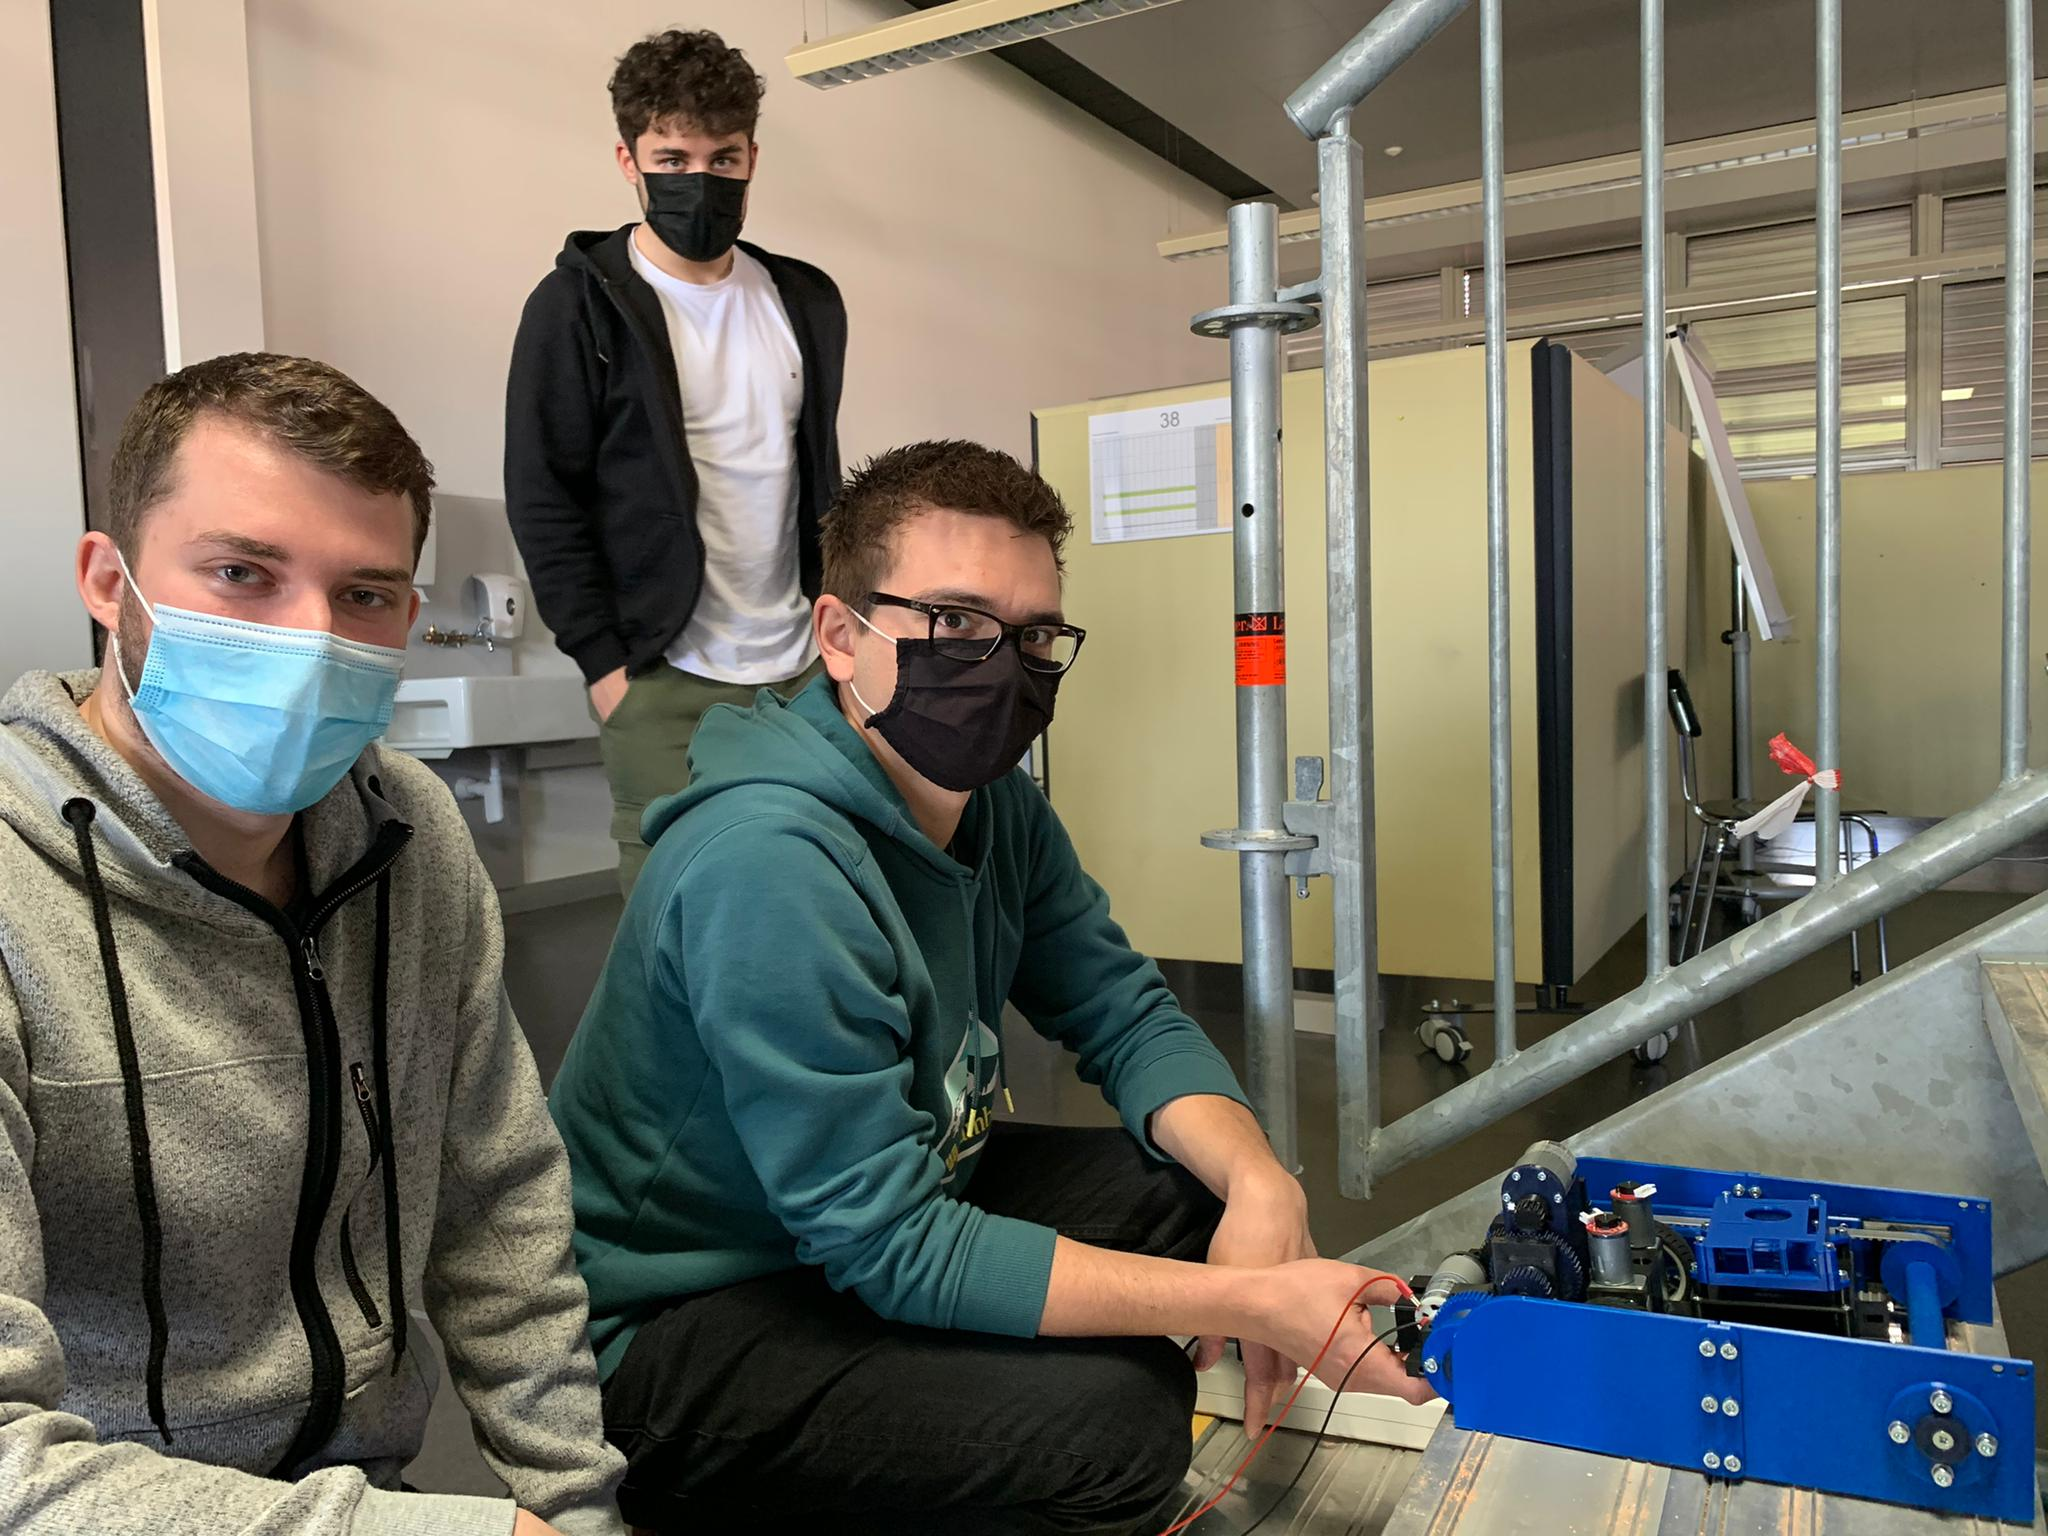
\includegraphics[width=0.65\textwidth]{img/Sprint1/pren1_sprint1_3.png}
  \centering
  \caption{Sprint 1 - Erste Treppentest}
  \label{fig:ersteTreppentests}
\end{figure}

Bei diesem Test konnte einiges über die Form der Ausleger und dessen Optimierungspotential gelernt werden.

Ein weiterer Punkt für Optimierungen sind die beiden Wellen die durch den Grundkörper verlaufen. Das Grundgerüst bestehend aus 3D-Druck Teilen erfüllt seinen Zweck vollumfänglich. Diese wurden durch Wellen aus Aluminium ausgetauscht. Dies, weil die Achsen für die Struktur von entscheidender Bedeutung sind. 

Der erste Sprint und somit die ersten Prototypentests haben Schwachstellen und Potential enthüllt. Das Konzept, das im \acrshort{pren1} erarbeitet wurde, ist umsetzbar. Es benötigt noch Optimierungen, um das volle Potential auszuschöpfen. Die Optimierungen wurden fortlaufend, neben dem Implementieren neuer Funktionen, umgesetzt.

\textbf{Fortbewegung:}

Die Fortbewegung soll möglichst auf engem Raum stattfinden können. Deshalb wurden in diesem Bereich zwei mögliche Drehmethoden getestet. Die einfachere der beiden ist das vor oder rückwärts drehen eines einzelnen Rades. Die etwas aufwändigere Methode ist das vor oder rückwärts drehen eines Rades während das andere Rad in die entgegengesetzte Richtung dreht.

Nach diesem Test hat sich ergeben, dass die zweite Variante mit dem ansteuern beider Motoren in unterschiedliche Richtungen eine Drehung nahezu auf einer Stelle gewährleistet. Somit wurde in der Software diese Art der Drehung implementiert.

\newpage

\subsection{Testing mit Software}\label{subsec:Fernbedienung}
Um einzelne Verhalten des Roboters wie beispielsweise die Hubbewegung oder die Ausrichtung auf der Treppe testen zu können, wurde zu Beginn der Python interactive Modus verwendet. Dies hat sich jedoch als zu langsam und ineffizient herausgestellt, weshalb daraufhin eine Fernbedienung über SSH realisiert wurde, mit welcher diese Funktionen schneller getestet werden konnten.
Mithilfe dieser Fernbedienung ist es möglich, den Roboter über die Tastatur des Notebooks zu steuern. Mit dem Notebook muss lediglich eine SSH Verbindung auf das Controllerboard mit dem embedded Linux hergestellt und das Python-Modul gestartet werden\texttt{remote\_control\_ssh.py}. Hierbei war die Schwierigkeit, dass Keyboard Inputs über SSH nicht direkt eingelesen werden können, wie das bei einer Tastatur welche direkt mit dem Controllerboard verbunden ist, der Fall ist. Dies aus dem Grund, dass Keyboardinputs nicht standardmässig über SSH übertragen werden. 

Dieses Problem konnte umgangen werden, indem auf dem Notebook ein X-Server \cite{Wikipedia-X-Window-System} gestartet und die SSH Verbindung mit einem X11-Forwarding erstellt wird. Das \texttt{remote\_control\_ssh.py} Modul startet dann ein Window auf dem X-Server welcher auf dem Notebook gestartet wurde. Die Keyboard Inputs werden dann über dieses Window bzw. diese X-Session eingelesen und an das Controllerboard übertragen. 

Als X-Server wurde der Xming X Server für Windows verwendet \cite{Xming-X-Window-Server-Download}.

Das X11-Forwarding bei der SSH Verbindung kann im Putty unter Connection/ssh/x11 enabled werden. 

\begin{figure}[H]
  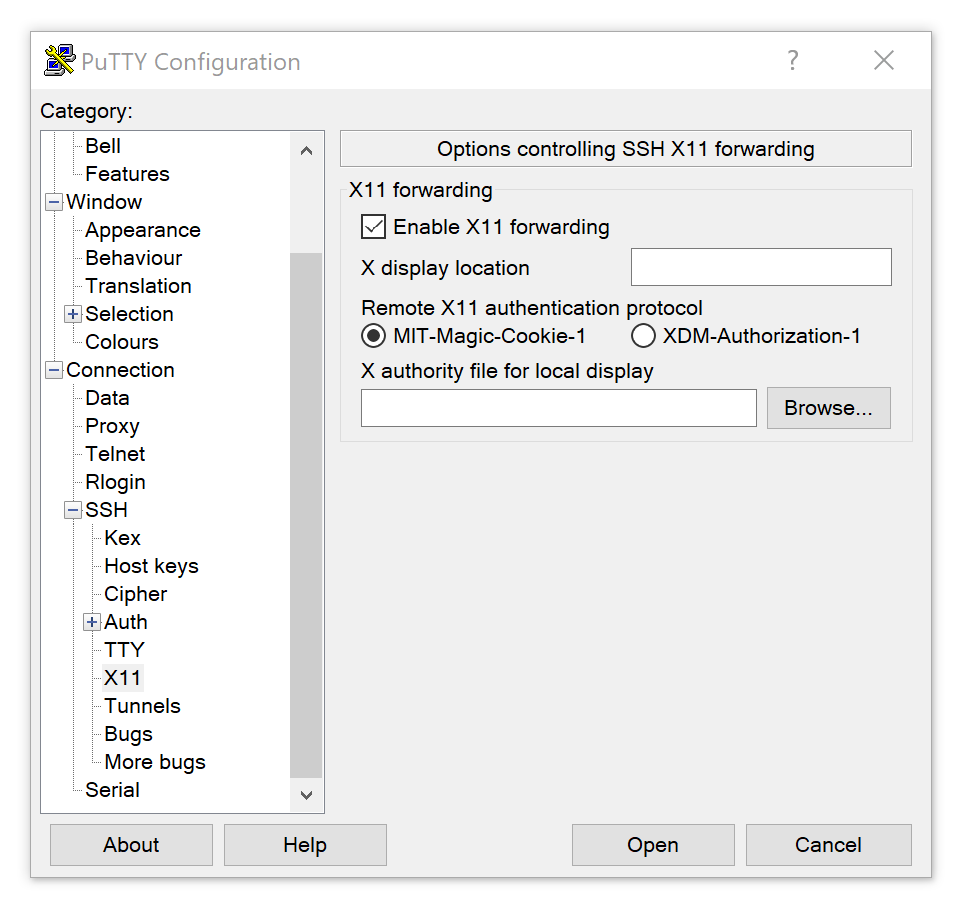
\includegraphics[width=0.65\textwidth]{img/remote_control/putty_x11.PNG}
  \centering
  \caption{Putty X11-Forwarding}
  \label{fig:putty_x11_forwarding}
\end{figure}


Bei einer SSH Verbindung aus der Konsole wird lediglich den Parameter -X (gross X) hinzugefügt. Der Befehl könnte dann folgendermassen aussehen: \texttt{ssh -X raspi\_hslu}.

Die Tastaturbelegung der Fernbedienung ist in Tabelle \ref{tab:tastaturbelegung-fernbedienung} abgebildet. Diese beinhaltete zu Beginn lediglich die Grundfunktionalitäten. Im Laufe des Projekts sind dann immer mehr für das Testing nützliche Befehle hinzu gekommen.\\

\begin{table}[H]
\centering
\begin{tabular}{|l|r|r|r|r|}
\hline
\textbf{Kommando} & \textbf{Tastaturbelegung} &
\textbf{Keycode}\\
\hline
Forward & W & 119\\
\hline
Backward & S & 115\\
\hline
Turn left & A & 97\\
\hline
Turn right & D & 100\\
\hline
Stop cruise & Q & 113\\
\hline
Main Motor Forward & E & 101\\ 
\hline
Main Motor Backward & R & 114\\ 
\hline
Main Stop & X & 120\\ 
\hline
Turn right 90 & F & 102\\ 
\hline
Turn left 90 & G & 101\\ 
\hline
Approach stair & 1 & 49\\ 
\hline
Align & 2 & 50\\ 
\hline
Climb step & 3 & 51\\ 
\hline
Tof distance & 4 & 52\\ 
\hline
Detect pictogram & 5 & 53\\ 
\hline
Calc pos infront stair & 6 & 54\\ 
\hline
Adjust pos infront stair & 7 & 55\\ 
\hline
Approach pictogram & 8 & 56\\ 
\hline
Align distance & 9 & 57\\ 
\hline
Acknowledge pictogram & 0 & 48\\ 
\hline
Straight forward 50cm & c & 99\\ 
\hline
Traverse & t & 116\\ 
\hline
Pathfind & p & 112\\ 
\hline
Emergency stop & [space] & 32\\ 
\hline
Quit & [esc] & 27\\ 
\hline
\end{tabular}
\caption[Tastaturbelegung für die Fernsteuerung]{Tastaturbelegung für die Fernsteuerung}
\label{tab:tastaturbelegung-fernbedienung}
\end{table}


\newpage

\textbf{Fortbewegung}

Die Fähigkeit, geradeaus zu fahren ist unter anderem für das Traversieren auf der Treppe von grosser Bedeutung, weshalb die Winkelmotoren der Fortbewegung spezifisch mit Encoder gewählt wurden. Mithilfe dieser Encoder können die Motoren so gesteuert werden, dass die Räder immer gleich schnell drehen. Dies wird in einer eigenen Klasse implementiert. Ebenfalls wird ein Modul programmiert, welches nach Eingabe eines Gradwertes eine möglichst genaue Drehung gewährleistet.

\begin{figure}[H]
  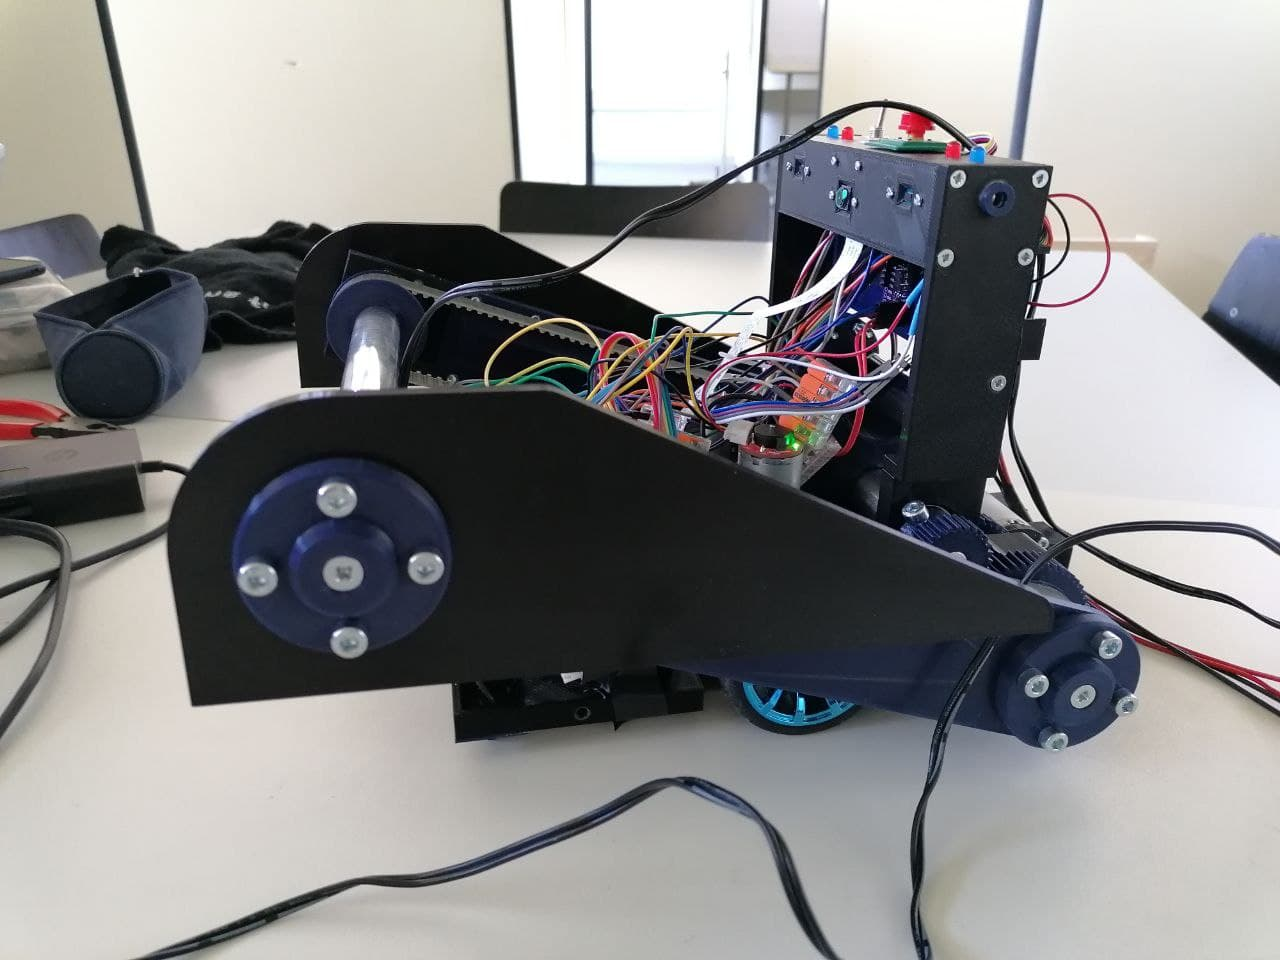
\includegraphics[width=0.65\textwidth]{img/Sprint3/fortbewegung.jpg}
  \centering
  \caption{Fortbewegungstests}
  \label{fig:Fortbewegungstests}
\end{figure}
In diesen Tests konnte festgestellt werden, dass aufgrund von dem geringen Schlupf zwischen dem Motor und den Rädern eine leichte Abweichung nicht umgangen werden kann. Dieser beläuft sich jedoch auf wenige Millimeter auf eine Fahrdistanz von 0.5 Meter. Somit kann ein zuverlässiges Geradeausfahren sichergestellt werden.

Beim Traversieren auf einer Treppenstufe werden die Rillen, die die Treppe aufweist, verwendet um nicht über die Kante einer Stufe zu fahren. Das Geradeausfahren auf einer Treppenstufe wird von den Halbkugelstützen, die entlang der Rillen gleiten, sichergestellt.

Die Drehung um die eigene Achse ist ein Punkt, bei welchem es viele Lösungsmöglichkeiten gibt. Das Ziel ist es, eine Drehung auf möglichst kleinem Raum zu ermöglichen. Dabei können die Räder verschieden schnell angesteuert werden um die Drehung zu optimieren. In den Tests hat sich ergeben, dass die Räder bereits in der Planung sehr gut plaziert wurden, weshalb die Räder gleichmässig angetrieben werden können ohne den Radius signifikant zu vergrössern.

\newpage

\textbf{Autonome Hubbewegung}

Der nächste Schritt ist die Automatisierung der Hubbewegung. Dazu werden weitere Komponenten im Grundgerüst verbaut und verkabelt. Dazu gehören neben den Motoren für die Hubbewegung auch die H-Brücken dieser Motoren. Ebenfalls werden bereits die Fortbewegungsmotoren mit der dafür vorgesehehenen H-Brücke verbunden. Weiter werden die Taster und der Schalter ausgemessen und Kabel angelötet um später Zeit einzusparen. Der Akku wird noch nicht verbaut aufgrund einer Lieferverzögerung, weshalb der erste Test noch mit einem Kabel zur Stromversorgung gemacht wird. Gesteuert wird der Roboter in diesem Versuch von einem Raspberry Pi 3B.
Auch wenn das Raspberry nicht der finale Controller des Roboters ist, können somit die in Python geschriebenen Funktionen getestet und verfeinert werden.
Das Ziel dieses Tests ist es, eine automatisierte, über den Controller gesteuerte Hubbewegung.

Dazu werden die ersten Tests auf einem Tisch durchgeführt und der Roboter abgefangen bevor der erste Treppentest durchgeführt wird.

\begin{figure}[H]
  \includegraphics[width=0.6\textwidth]{img/Sprint2/pren2-Löten.jpg}
  \centering
  \caption{Verkabelung der Elektronikkomponenten}
  \label{fig:verkabelung-elektronik}
\end{figure}

\newpage

Zu Beginn werden alle Komponenten des Roboters einzeln über den Controller angesteuert und getestet, wie sich diese verhalten. Dabei fällt auf, dass die menschliche Reaktionszeit der beschränkende Faktor ist beim Erklimmen der Treppe. Eine Hubbewegung ist möglich aber nur sehr langsam. Um die Hubbewegung vollkommen autonom gewährleisten zu können werden die einzelnen Module in Verhalten eingeteilt welche eine Aufgabe erledigen und dazu die Module eigenständig verwendet.\\



\textbf{Anfahren der Treppe}

Um an die Treppe heranfahren und sich ausrichten zu können, werden die Module der Fortbewegung in Kombination mit den beiden TOF-Sensoren benötigt, welche auf Höhe der Treppenkante montiert sind. Die Sensoren liefern dabei nicht nur die Werte für die Distanz zur Treppe sondern auch die Ausrichtung zur Treppe. Ist der Abstand zur Treppe wie gewünscht, stoppt das Gerät und dreht sich noch soweit um die eigene Achse, bis der Distanzunterschied beider Sensoren im vorbestimmten Toleranzbereich ist und der Roboter somit für die nächste Hubbewegung bereit ist.
Der Controller startet das Verhalten zum Anfahren und Ausrichten zur Treppe, welches wiederum die programmierten Module verwendet. Dieser Aufbau der Software ermöglicht ein sehr flexibles Vorgehen und eine gute Überschaubarkeit des Codes.

\begin{figure}[H]
  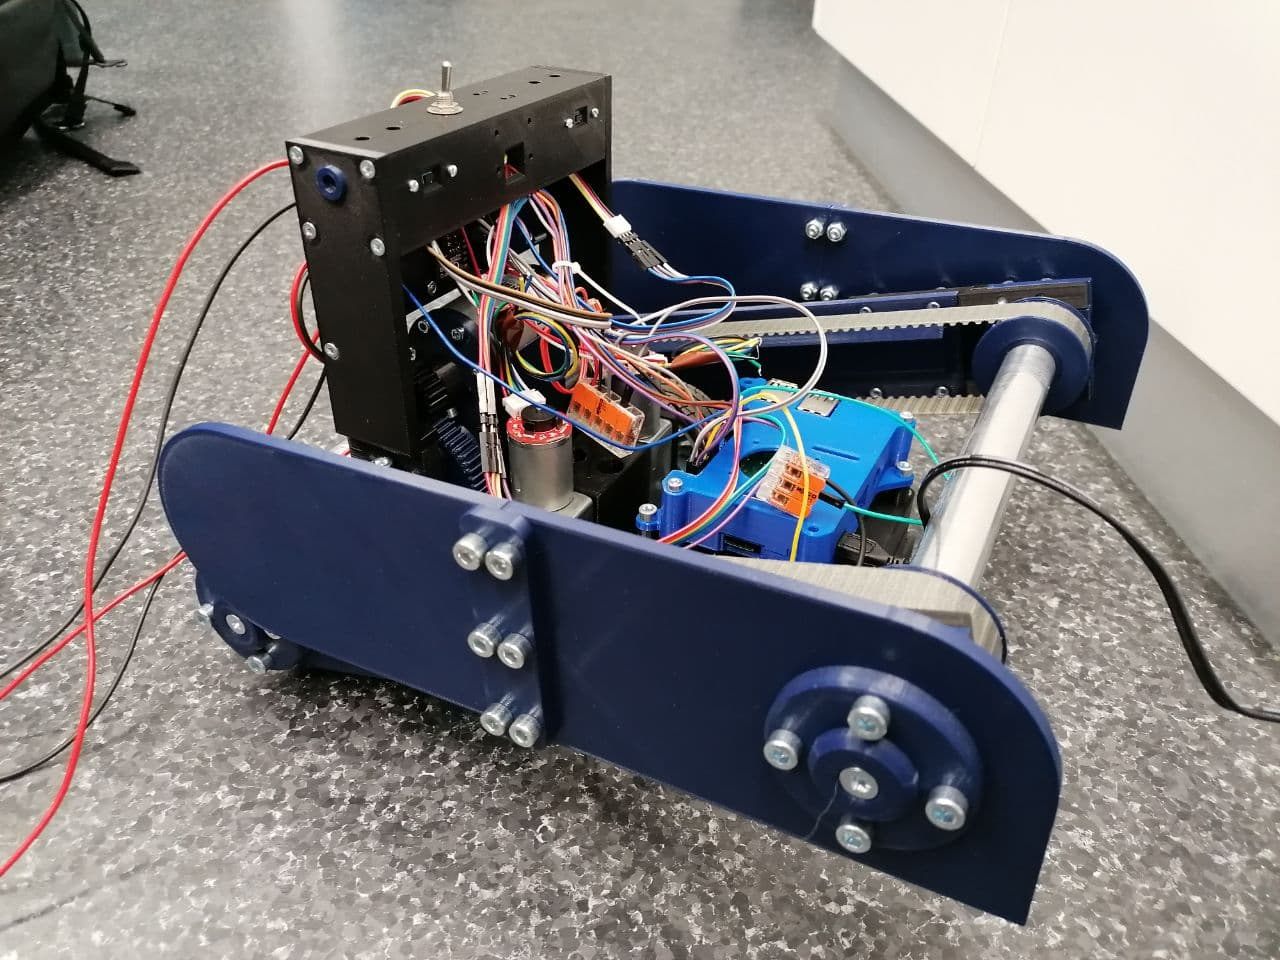
\includegraphics[width=0.65\textwidth]{img/Sprint2/pren2_ausrichten-anfahren.jpg}
  \centering
  \caption{Roboter beim Test zur automatischen Ausrichtung}
  \label{fig:automatische-ausrichtung}
  \end{figure}
  
\newpage
  
\textbf{Bilderkennung}

Um den Pfad zu berechnen, müssen die Hindernisse auf der Treppe gefunden werden. Dazu wird eine Datenbank mit möglichst vielen Bildern gesammelt, auf welchen die Ziegelsteine manuell eingezeichnet werden. Die Datenbank umfasst ungefähr 420 Bildern und ermöglicht dem Computer somit eine zuverlässige Vergleichsbasis, um die Hindernisse selbstständig zu finden. Diese Bilder werden mit einem Mock-Up und einer selber entwickelten App gemacht, um einerseits die Kamera auf der richtigen Höhe zu fixieren und andererseits, um die Handhabung zu vereinfachen.

\begin{figure}[H]
  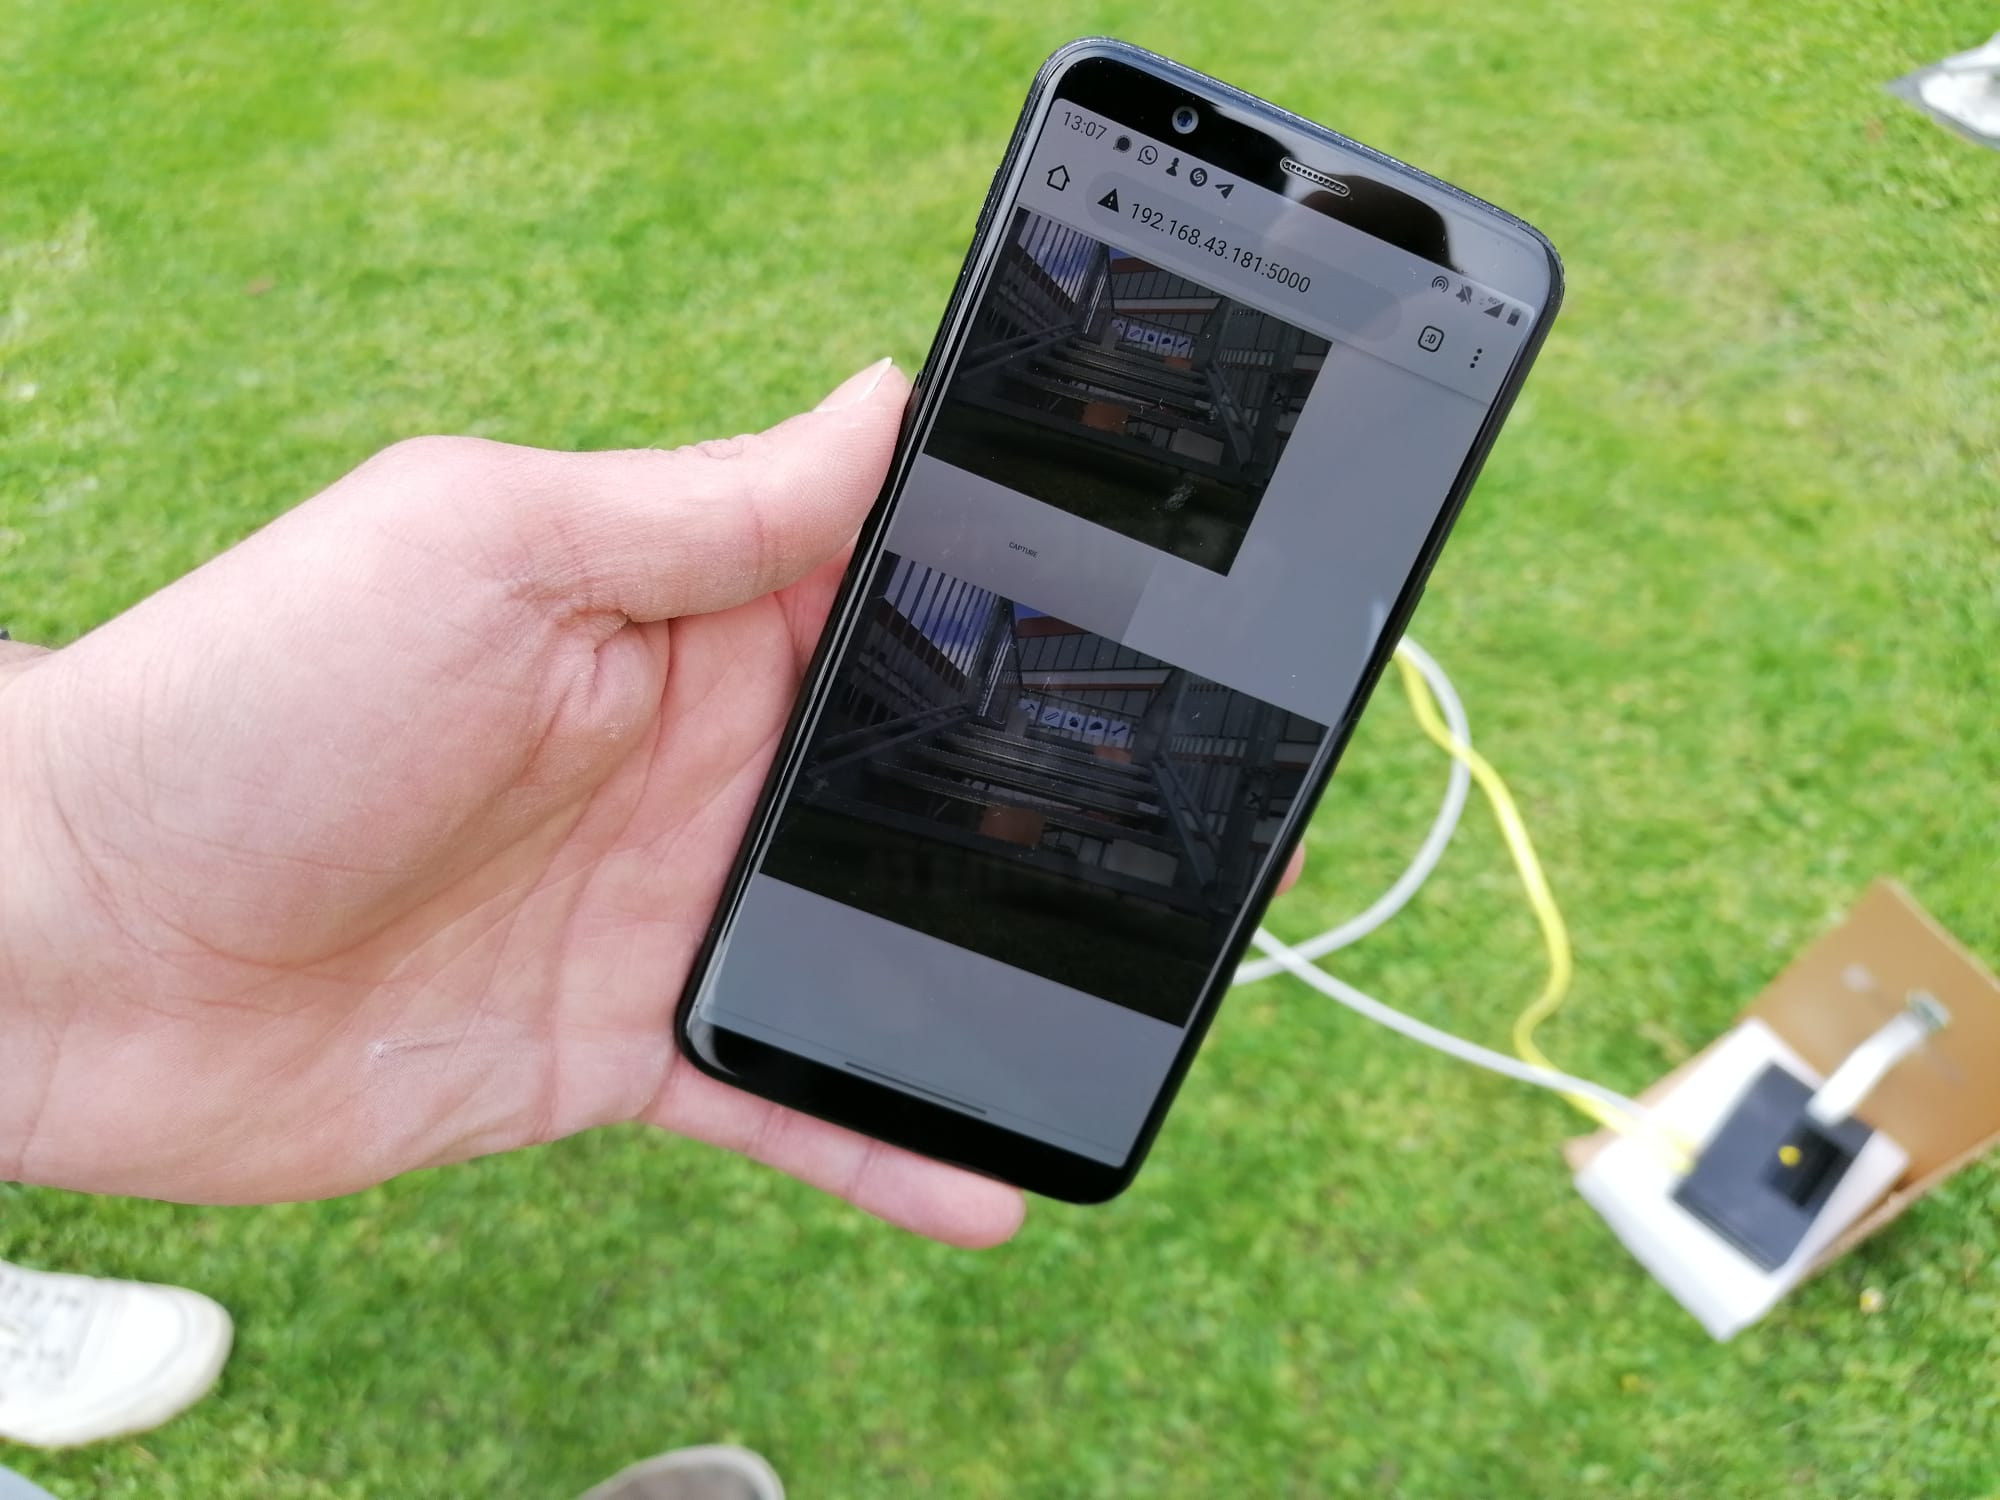
\includegraphics[width=0.5\textwidth]{img/Sprint3/Sprint3_Bildersammlung.jpeg}
  \centering
  \caption{Aufnahme von Referenzbildern}
  \label{fig:Aufnahme der Referenzbilder}
  \end{figure}
  
Zusätzlich werden Bilder für die Piktogrammerkennung im Start- und Zielbereich gemacht. Dies wiederum, um den bereits erstellten Piktogrammerkennungsalgorithmus zu testen und zu verfeinern.
  
  \begin{figure}[H]
  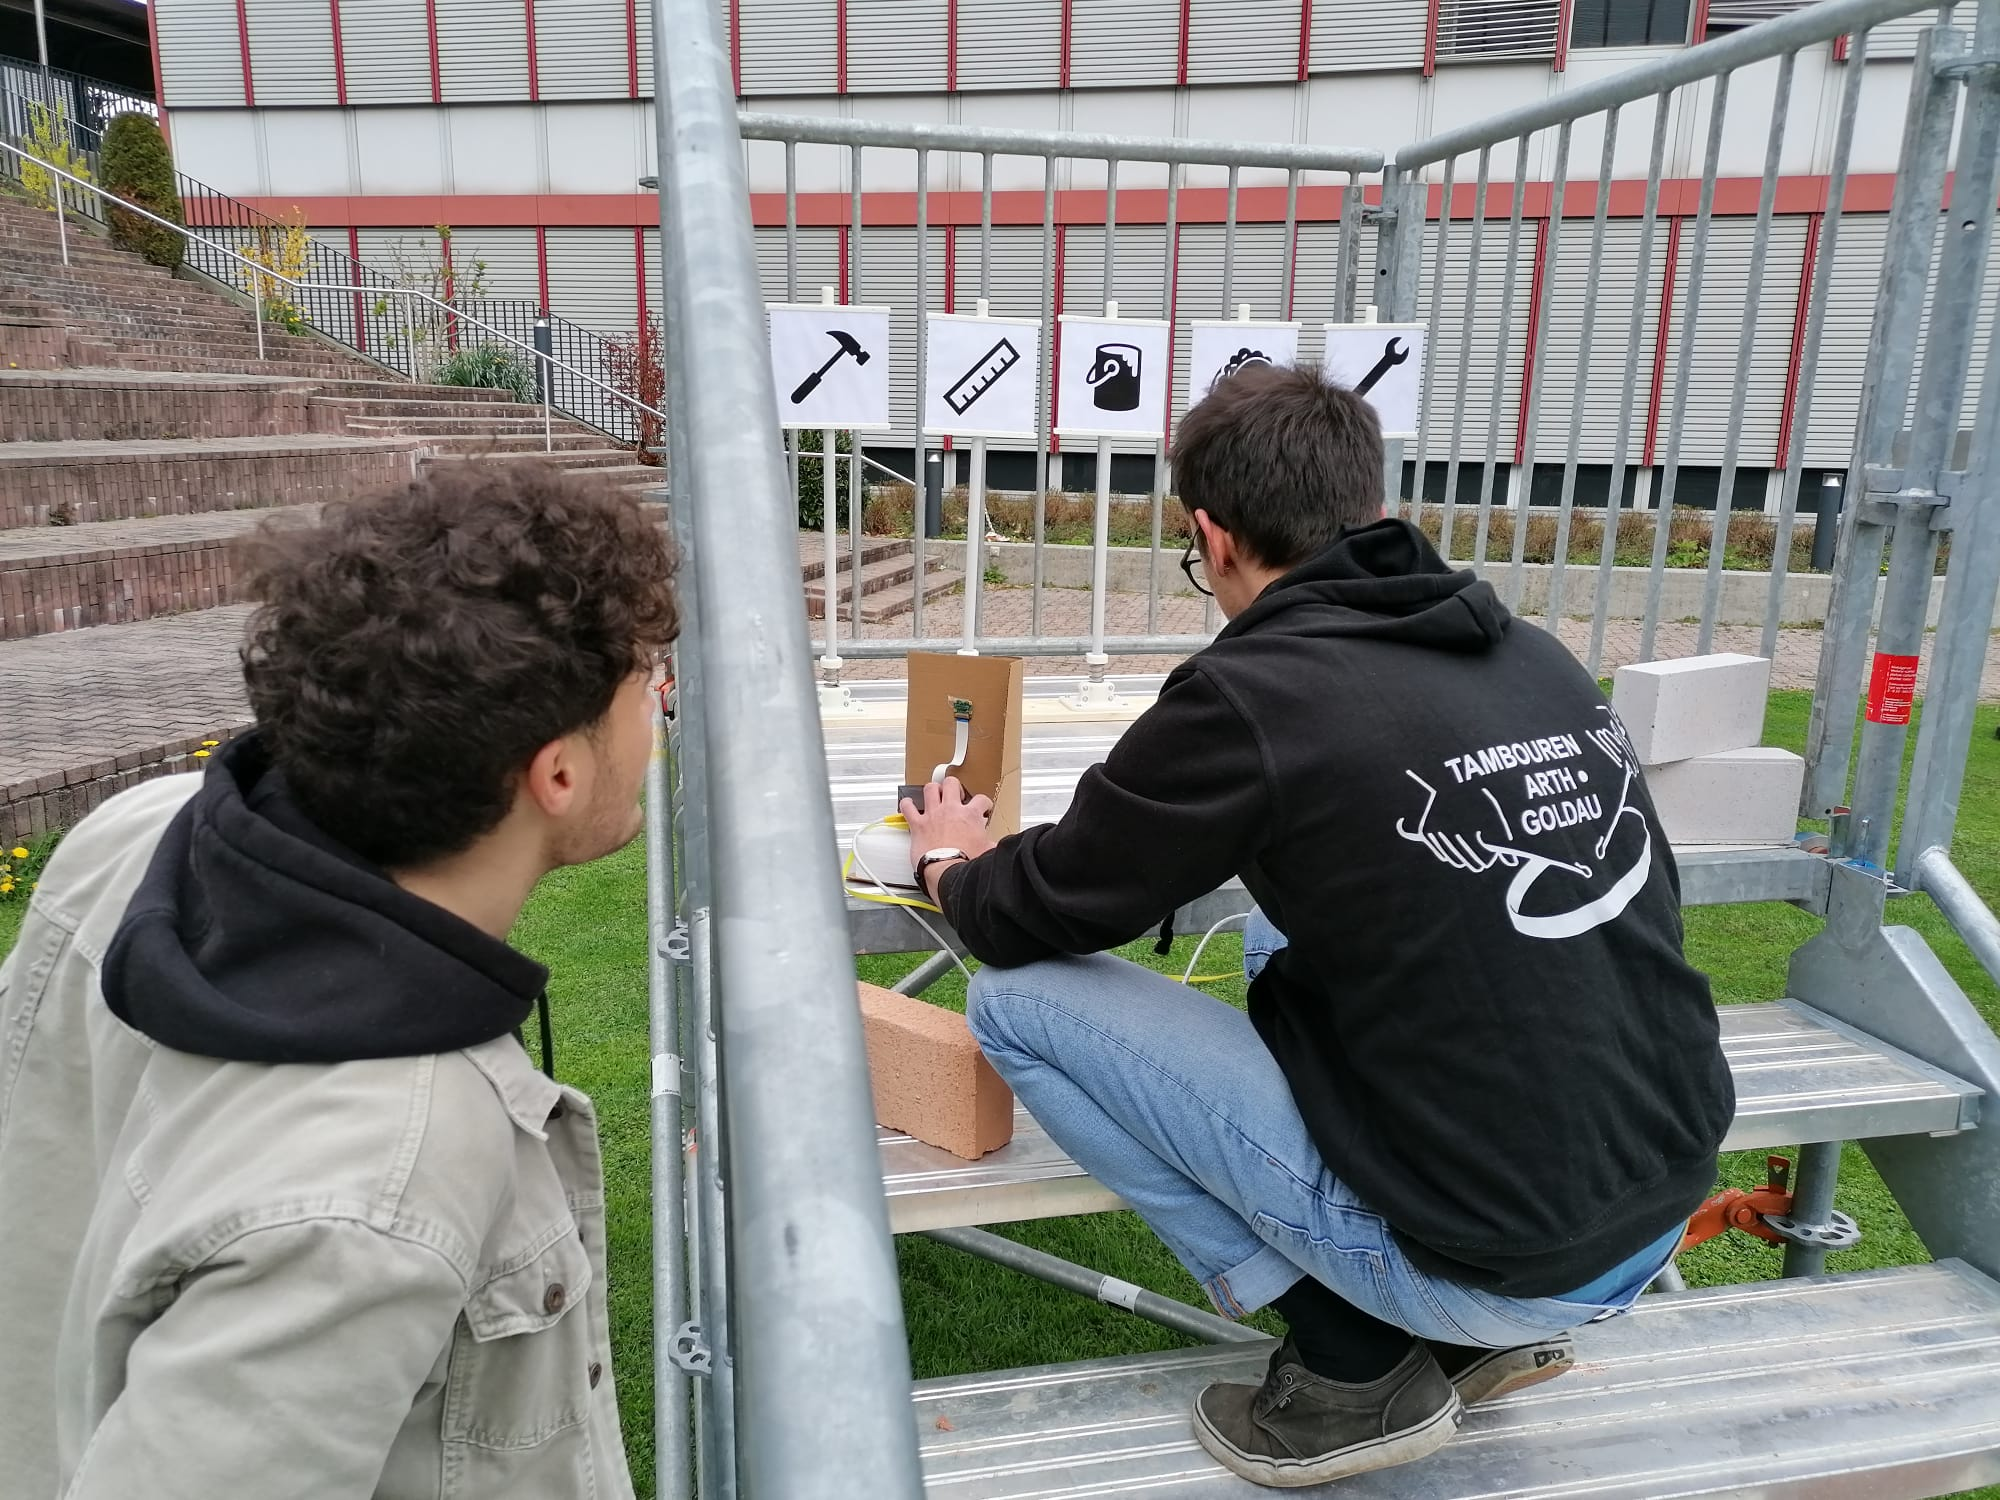
\includegraphics[width=0.5\textwidth]{img/Sprint3/Sprint3_Bildersammlung2.jpeg}
  \centering
  \caption{Das Team bei der Aufnahme der Referenzbilder}
  \label{fig:Aufnahmeprozess der Referenzbilder}
  \end{figure}
  
\newpage

\textbf{Funktionsweise mit Akku}\label{sec:Funktionsweisemit Akku}

Um ein autonomes Fahren gewährleisten zu können, muss der Roboter mit einem Akku betrieben werden können. Dazu werden verschiedene Schritte benötigt. Ausserdem wird erstmals das Jetson Nano verwendet.

\begin{figure}[H]
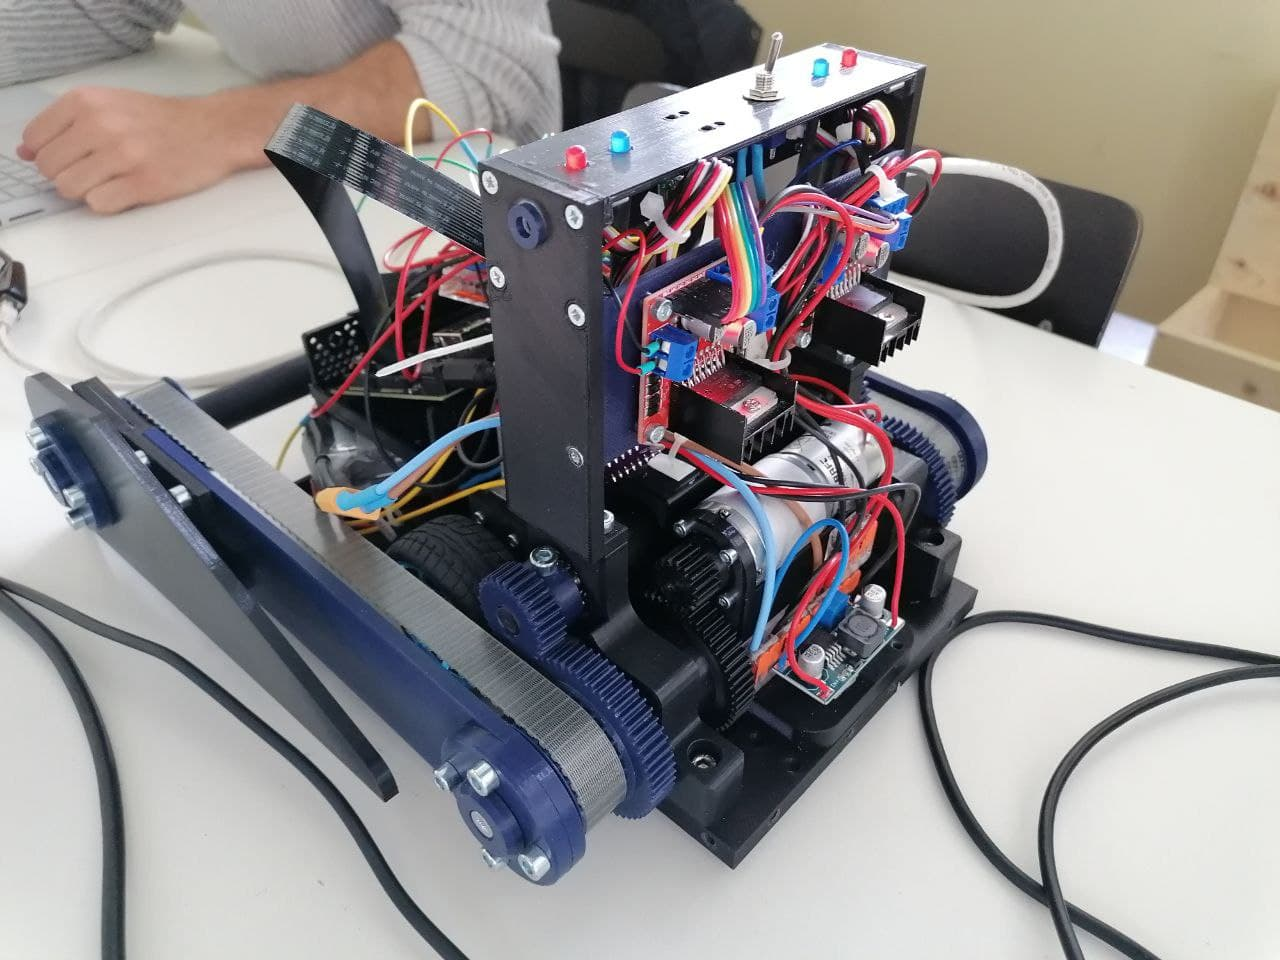
\includegraphics[width=0.7\textwidth]{img/Sprint3/Sprint3_Verkabelung1.jpg}
\centering
\caption{Rückansicht der ersten Verkabelung mit Akku} \label{fig:Rückansicht der ersten Verkabelung}
\end{figure}
  
  
In einem ersten Schritt werden die zwei Spannungslevel hergestellt. Der Akku liefert 16 Volt, welche für alle Motoren verwendet werden. Mithilfe des Wandlers wird das zweite Niveau von 5 Volt erreicht, welches neben dem Jetson auch sämtliche Sensoren unabhängig des Controllers mit Strom versorgt. So kann das Jetson den zur Verfügung gestellten Strom für die volle Leistung verwenden.
Die Verkabelung sämtlicher Elemente ist provisorisch. Geplant ist, dass das Kabelmanagement nach Abschluss der Funktionskontrolle aller Elemente verbessert wird, um zu einem späteren Zeitpunkt einen besseren Überblick zu gewährleisten.
  
\begin{figure}[H]
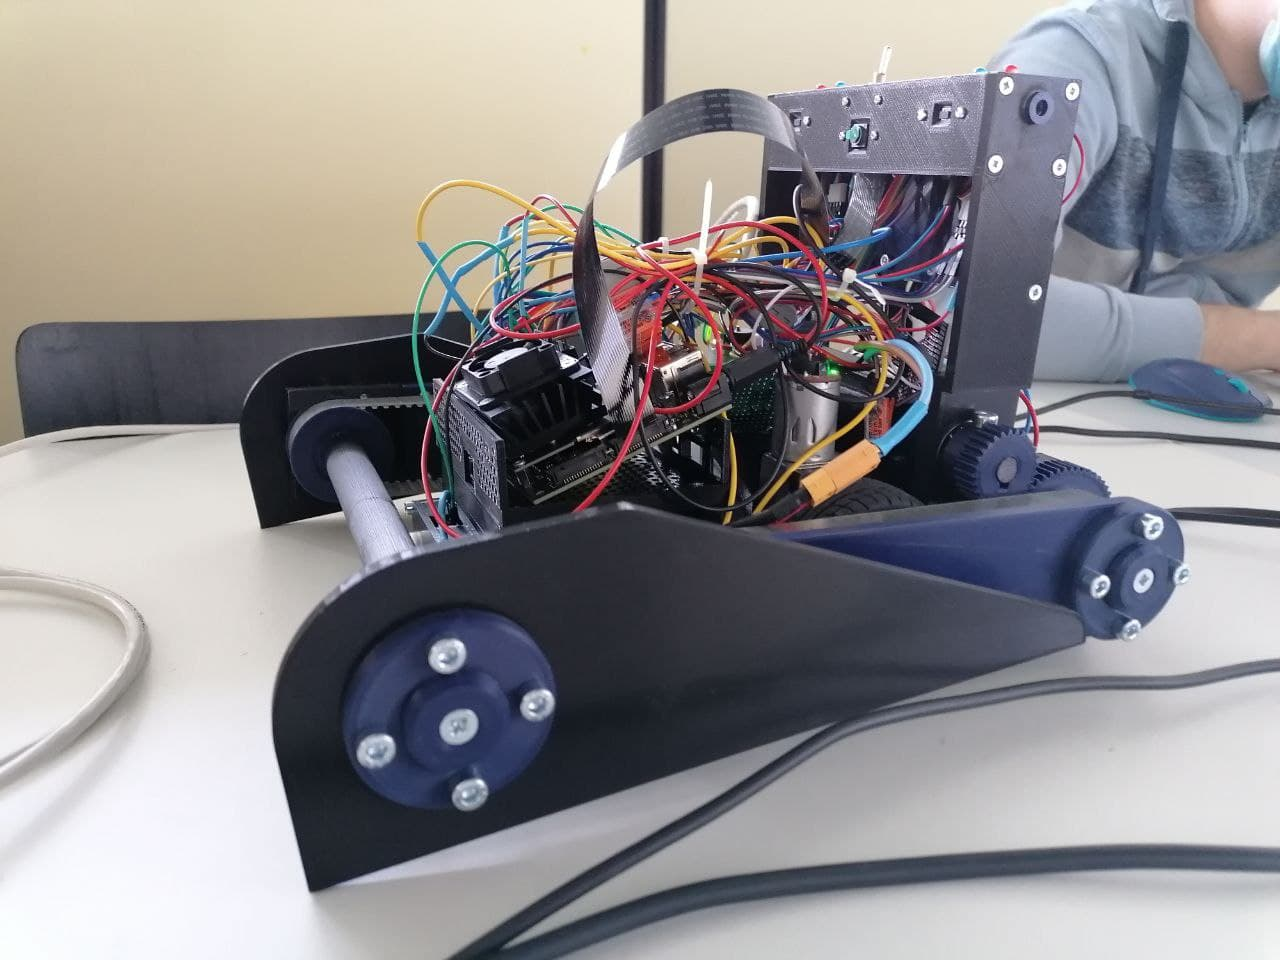
\includegraphics[width=0.65\textwidth]{img/Sprint3/Sprint3_Verkabelung2.jpg}
\centering
\caption{Seitenansicht der ersten Verkabelung mit Akku}
\label{fig:Seitenansicht der ersten Verkabelung}
\end{figure}
  
Der Not-Aus-Schalter der fertigen Konstruktion schaltet wie geplant nur die H-Brücken der Motoren. Die 5 Volt Spannungsverteilung wird vom Schalter nicht tangiert. Dies um zu umgehen, dass das Jetson Nano ohne korrektes Herunterfahren abgeschaltet wird.
  
Zusätzlich wurde der Hilfsmotor der Hubbewegung entfernt und der Hauptmotor der Hubbewegung weiter nach vorne verlagert. So kann der Schwerpunkt nach vorne verschoben werden. Der Hilfsmotor wurde entfernt, da die Stufenerklimmung auch ohne Einklappen der Standfüsse der Ausleger funktioniert. Dazu musste aber die Auslegerwelle wieder mit einer 3D gedruckten Welle ersetzt werden, um das Gewicht der Ausleger reduzieren zu können, dass die Stufenerklimmung funktioniert. Die Welle 2, die vom Hilfsmotor angetrieben wurde, konnte weiter verwendet werden. Die Konstruktion der Welle 2 wurde beibehalten, nur wurde sie fixiert, dass sie sich nicht drehen kann.
  
Ergebnisse: Mithilfe der Gewichtsreduktion kann die Hubbewegung schneller, einfacher und nur noch mit einem Motor durchgeführt werden. Das Pathfinding wurde mithilfe der über 300 Referenzbilder trainiert und liefert überzeugende Ergebnisse.
 
\textbf{Einbindung des Jetson Controller}

Um das Jetson einbinden zu können, müssen die Module der Software auf die Jetson-Libraries umgeschrieben werden. Dazu werden die Module der State-Machine auf eine GPIO-Library, welche vom Jetson unterstützt wird, reduziert. Da das Jetson kein eingebundenes WLAN-Modul besitzt, werden für die Tests ein externes WLAN Modul eingebunden um den Roboter weiterhin remote steuern und updaten zu können.
 
Zusätzlich wird ein externer PWM Verteiler verwendet, da das Jetson nur über zwei PWM Ausgänge verfügt. Somit können alle Motoren über Hardware-PWM Pins angesteuert werden als im Vergleich zum Raspberry Pi über Software PWMs. 
 
\newpage
 
\textbf{Modultests auf Originaltreppe}

Um die Module korrekt testen zu können, werden Tests auf der Originaltreppe im Aussenbereich durchgeführt. Dies um in erster Linie den Einfluss verschiedenen Lichtverhältnisse auf die Kamera und die Sensoren zu überprüfen. In diesen Tests konnte auch erstmals das optimierte Pfadfindungsmodul auf der entscheidenden Treppe gemacht werden.

   \begin{figure}[H]
  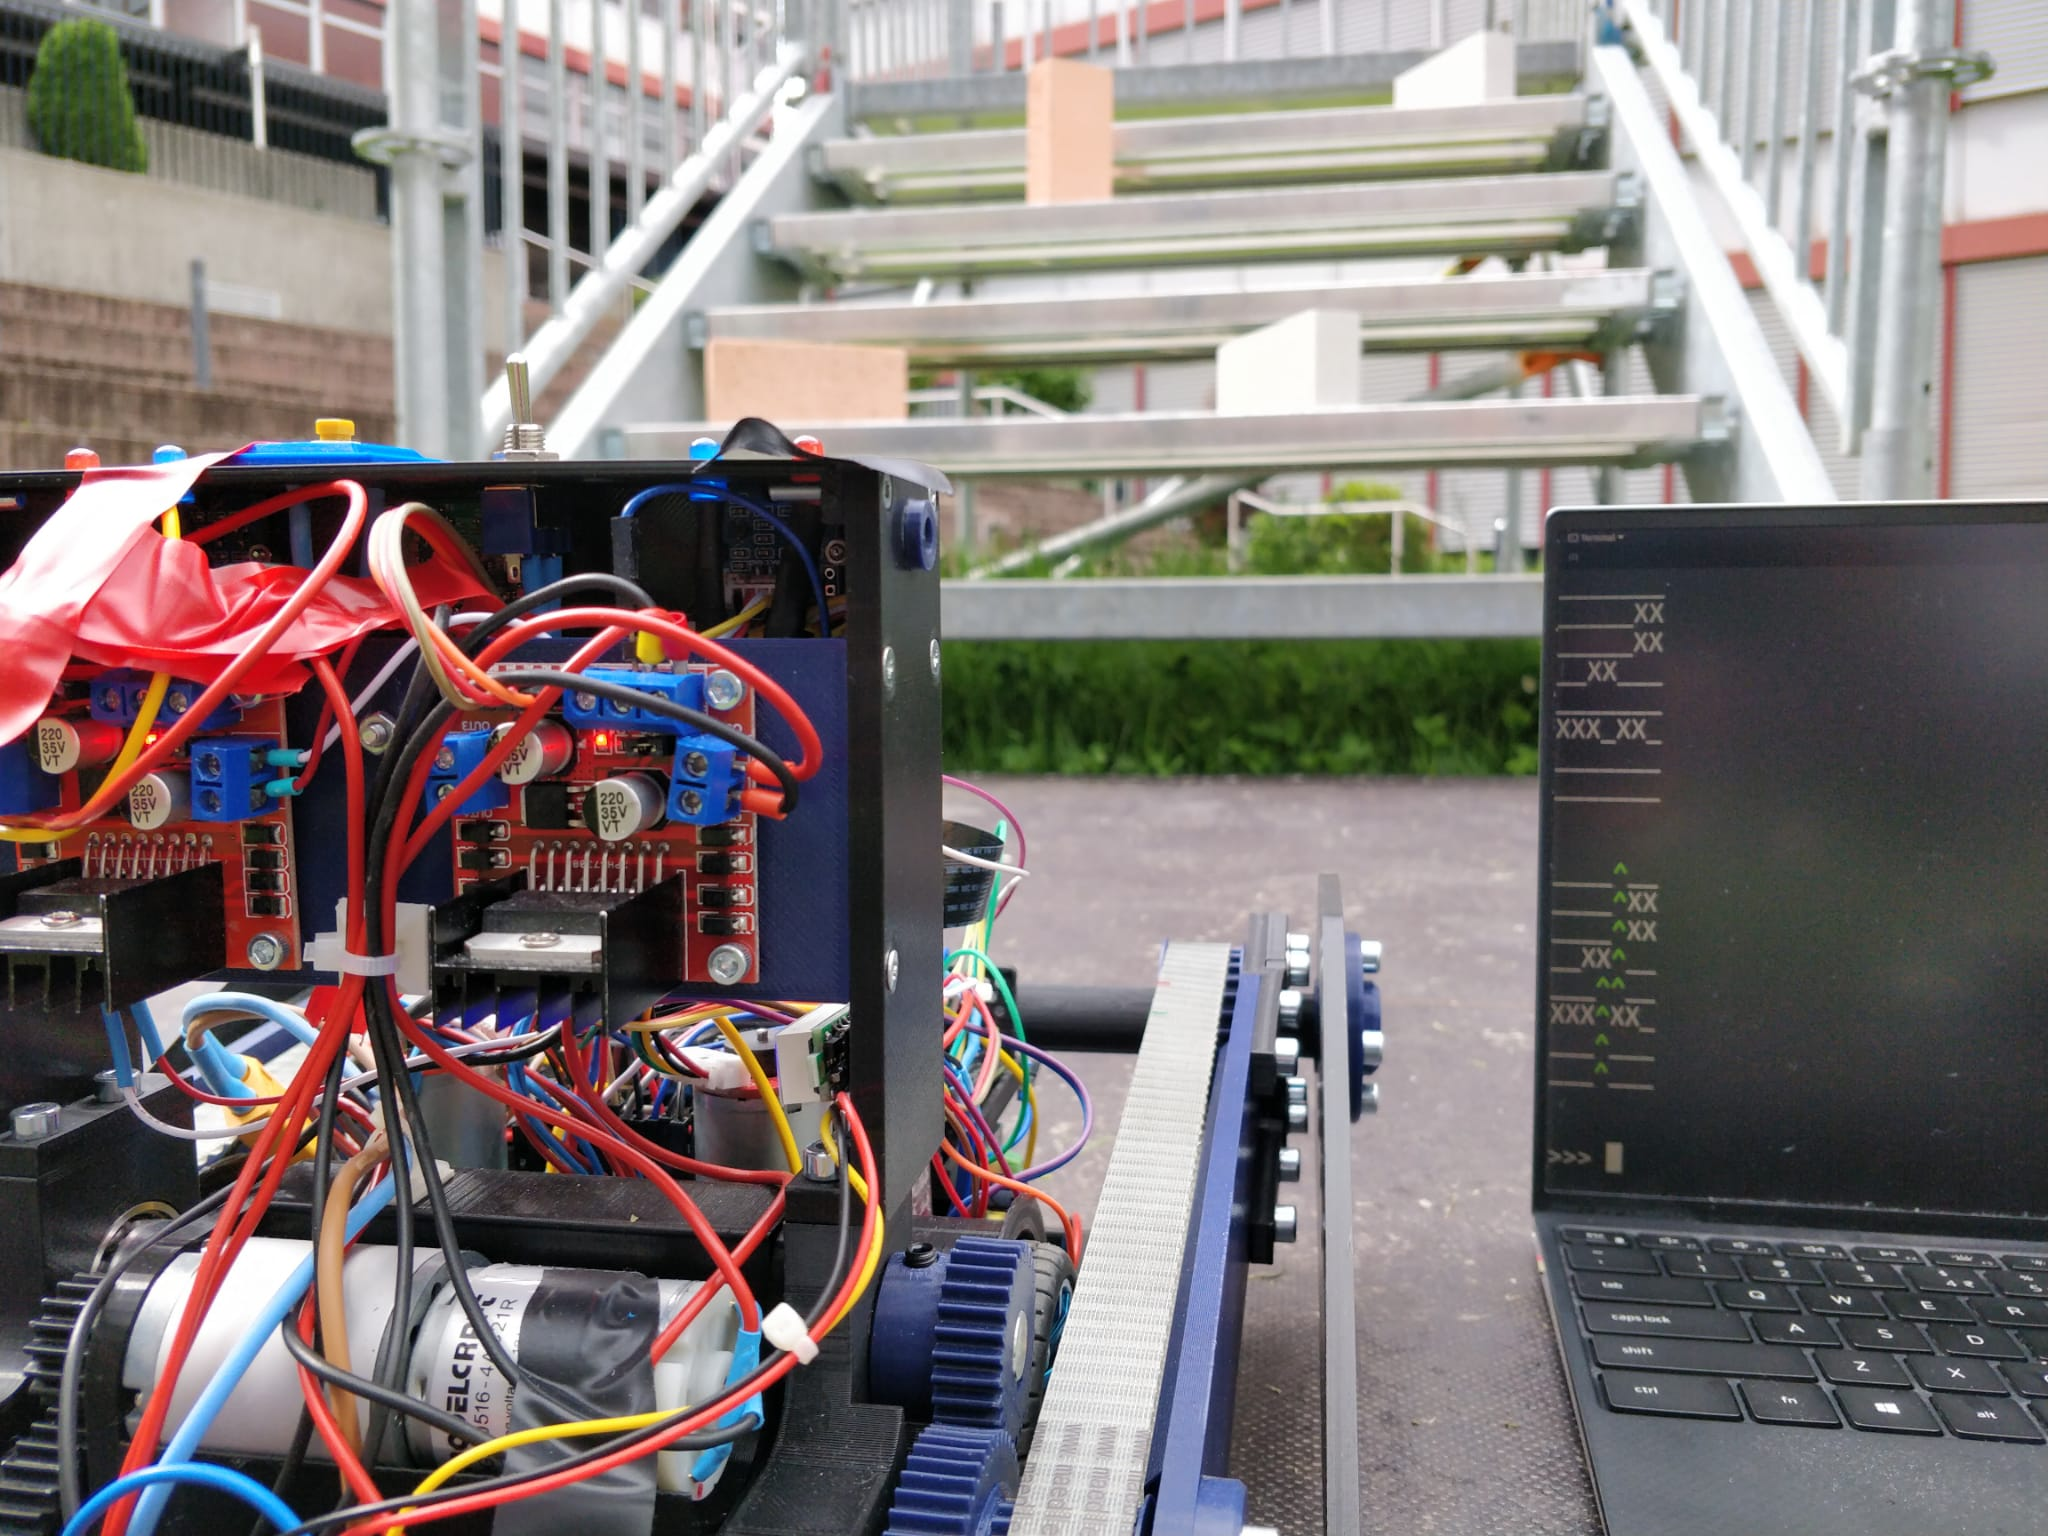
\includegraphics[width=0.7\textwidth]{img/Sprint3/pren2_tests_treppe.jpeg}
  \centering
  \caption{Pfadfindungtests auf Originaltreppe}
  \label{fig:Tests auf Originaltreppe}
  \end{figure}
  
  Bei diesen Tests hat sich auch gezeigt, dass die TOF-Sensoren auf der leicht reflektierenden Treppe eine grosse Ungenauigkeit aufweisen. Bei den Versuchen wurde eine Messgenauigkeit von +-10cm ersichtlich. Aus diesem Grund wurden die Time of Flight Sensoren mit Ultraschallsensoren ersetzt. Dies ist verhältnismässig einfach gelungen, da beim Aufbau der Software konsequent mit Interfaces und Dependency Injection gearbeitet wurde. Somit musste anstelle der TOF-Module nur die bereits existierenden Ultraschall-Module in den AlignmentChecker injecten werden. Es wurden somit keinerlei Codeänderungen benötigt.
  
  Da die Flugzeit der Ultraschallsensoren jedoch auf einem nicht Realtime System berechnet werden muss 
\footnote{\url{https://en.wikipedia.org/wiki/Real-time_operating_system}}, haben auch diese eine gewisse Messungenauigkeit.
  Um diese Ungenauigkeit zu minimieren, wurde die Berechnung vom Python Programm in ein Kernelmodul\footnote{
    \url{https://github.com/johannesthoma/linux-hc-sro4}
  } verlagert, dies gibt wesentlich genauere Messdaten zurück.
  
 Somit ist folgend der Roboter mit der finalen Hardware dargestellt.
 
    \begin{figure}[H]
  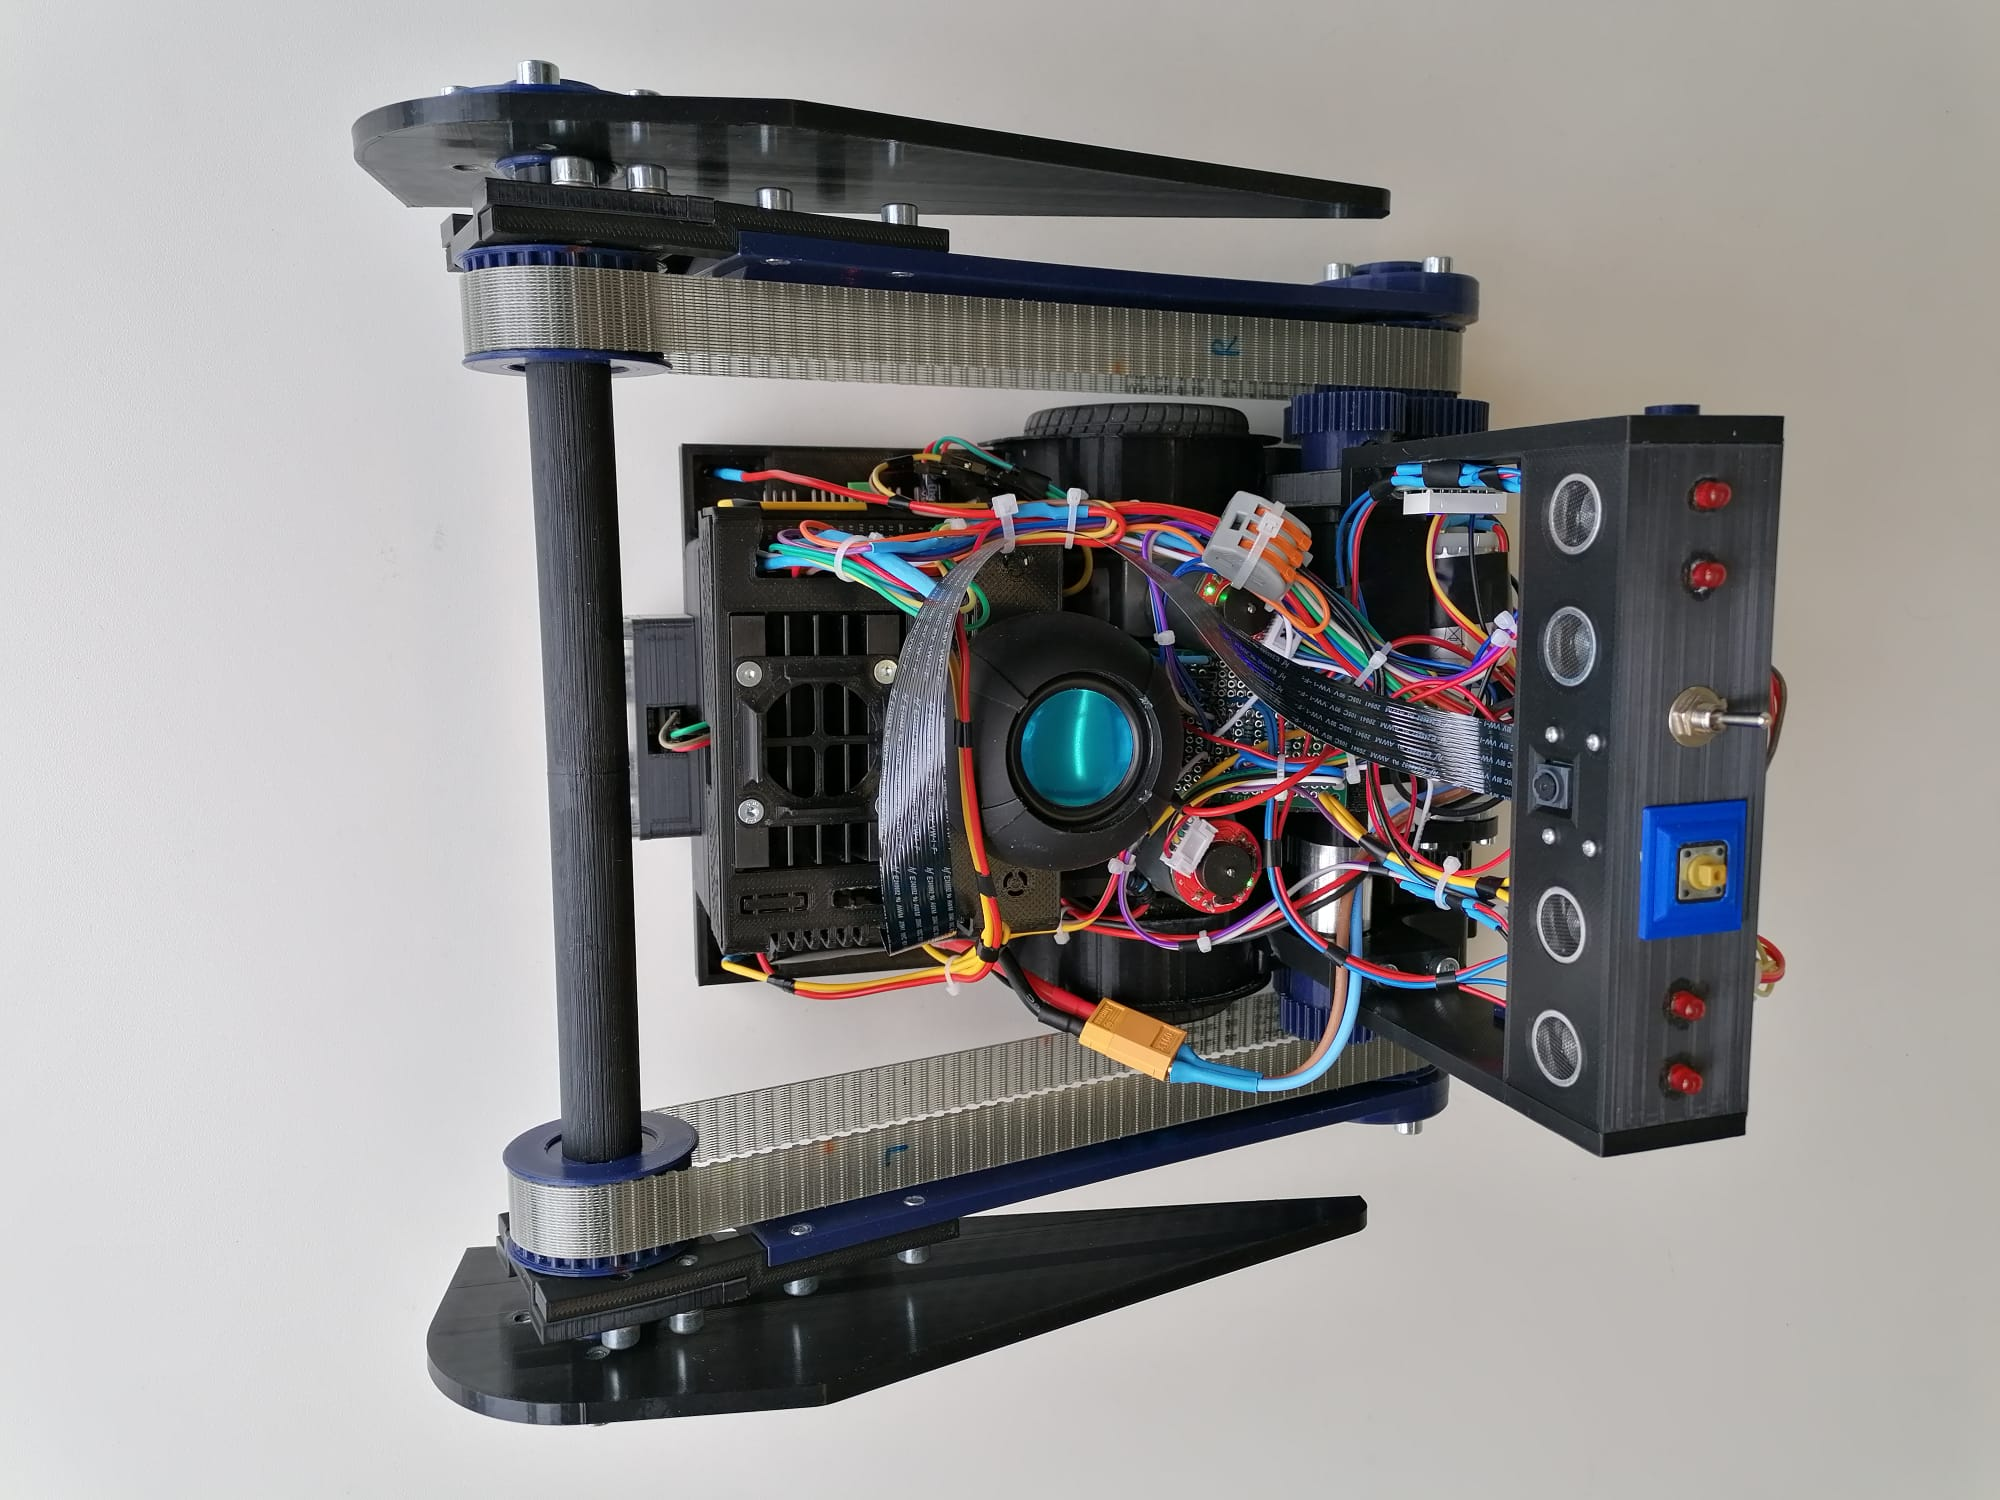
\includegraphics[width=0.9\textwidth]{img/Sprint3/pren2_tests_treppe2.jpeg}
  \centering
  \caption{Finale Hardware}
  \label{fig:Tests auf Originaltreppe1}
  \end{figure}
 
 
  
  
  
  
  
  
  
  
  





  